%\documentclass[a4paper,11pt]{book}
\documentclass[a4paper,twoside,11pt,titlepage]{book}

\usepackage[top=2.5cm, bottom=2.5cm,
            left=2.5cm, right=2.5cm, twoside]{geometry}



%\usepackage{doxygen/doxygen}
%\usepackage{pdfpages}
\usepackage{url}
\usepackage[spanish,es-noshorthands]{babel}
\usepackage{colortbl,longtable}
\usepackage[stable]{footmisc}
%\usepackage{index}
%\usepackage[chapter]{algorithm}
\RequirePackage{verbatim}
%\RequirePackage[Glenn]{fncychap}
\usepackage{fancyhdr}
\usepackage[hidelinks]{hyperref} %referencia
\usepackage{graphicx}
\usepackage{svg}
\usepackage{afterpage}
\usepackage[acronyms,toc]{glossaries}
\usepackage{longtable}
\usepackage{multicol}
\usepackage{import}
\usepackage{booktabs}
\usepackage{stackengine}
\usepackage{circuitikz}
\usepackage{tikz}
\usepackage{pgfplots}
\usepackage{subcaption}
\usepackage{rotating}
\usepackage{eurosym}
\usepackage{amsfonts}
\usepackage{amsmath}
\usepackage[toc,page]{appendix}
\usepackage{listings}
\usepackage[utf8]{inputenc}
\usepackage{caption}
\usepackage[spanish,es-tabla]{babel}
\usepackage[framed,numered]{matlab-prettifier}

\makeglossaries
\makeindex

%\usepackage{titlesec}
%\usepackage{pailatino}

\decimalpoint
\usepackage{dcolumn}
\newcolumntype{.}{D{.}{\esperiod}{-1}}
\makeatletter
\addto\shorthandsspanish{\let\esperiod\es@period@code}
\makeatother

%\usepackage{doxygen/doxygen}
%\usepackage{pdfpages}
\usepackage{url}

\usepackage{colortbl,longtable}
\usepackage[stable]{footmisc}
%\usepackage{index}
%\usepackage[chapter]{algorithm}
\RequirePackage{verbatim}
%\RequirePackage[Glenn]{fncychap}
\usepackage{fancyhdr}
\usepackage[hidelinks]{hyperref} %referencia
\usepackage{graphicx}
\usepackage{afterpage}
\usepackage{glossaries}
\usepackage{longtable}
\usepackage{xspace}
\usepackage{float}

\makeindex
\makeglossaries



% ********************************************************************
% Re-usable information
% ********************************************************************
\newcommand{\myTitle}{Título de mi proyecto\xspace}
\newcommand{\myDegree}{Grado en Ingeniería de Tecnologías de Telecomunicación\xspace}
\newcommand{\myName}{Juan Ordóñez Cerezo\xspace}
\newcommand{\myProf}{Encarnación Castillo Morales\xspace}
\newcommand{\myOtherProf}{Jose María Cañas Plaza \xspace}
%\newcommand{\mySupervisor}{Put name here\xspace}
\newcommand{\myFaculty}{Mi facultad}
\newcommand{\myFacultyShort}{\xspace}
\newcommand{\myDepartment}{Departamento de Electrónica y Tecnología de Computadores \xspace}
\newcommand{\myUni}{\protect{Universidad de Granada}\xspace}
\newcommand{\myLocation}{Granada\xspace}
\newcommand{\myTime}{\today\xspace}
\newcommand{\myVersion}{Version 0.1\xspace}


\hypersetup{
pdfauthor = {\myName (email (en) ugr (punto) es)},
pdftitle = {\myTitle},
pdfsubject = {},
pdfkeywords = {},
pdfcreator = {LaTeX con el paquete ....},
pdfproducer = {pdflatex}
}

%\hyphenation{}


%Definición de comandos que me son tiles:

\DeclareCaptionSubType[alph]{figure}
\captionsetup[subfigure]{labelformat=simple,justification=centerlast}
\renewcommand\thesubfigure{\alph{subfigure})}

\renewcommand{\indexname}{Índice alfabético}
\renewcommand{\glossaryname}{Glosario}
\renewcommand{\acronymname}{Acrónimos}
\renewcommand{\tablename}{Tabla}

\makeatletter
\renewcommand\p@subfigure{\thefigure~}
\makeatother


\addto\extrasspanish{%
  \renewcommand{\chapterautorefname}{Capítulo}%
  \renewcommand{\sectionautorefname}{Sección}
}

%Encabezados
\pagestyle{fancy}
\fancyhf{}
\fancyhead[LO]{\leftmark}
\fancyhead[RE]{\rightmark}
\fancyhead[RO,LE]{\textbf{\thepage}}
\renewcommand{\chaptermark}[1]{\markboth{\textbf{#1}}{}}
\renewcommand{\sectionmark}[1]{\markright{\textbf{\thesection. #1}}}

\setlength{\headheight}{1.5\headheight}

\newcommand{\HRule}{\rule{\linewidth}{0.5mm}}

%Definimos los tipos teorema, ejemplo y definición podremos usar estos tipos
%simplemente poniendo \begin{teorema} \end{teorema} ...
\newtheorem{teorema}{Teorema}[chapter]
\newtheorem{ejemplo}{Ejemplo}[chapter]
\newtheorem{definicion}{Definición}[chapter]

\definecolor{gray97}{gray}{.97}
\definecolor{gray75}{gray}{.75}
\definecolor{gray45}{gray}{.45}
\definecolor{gray30}{gray}{.94}

\lstset{ frame=Ltb,
     framerule=0.5pt,
     aboveskip=0.5cm,
     framextopmargin=3pt,
     framexbottommargin=3pt,
     framexleftmargin=0.1cm,
     framesep=0pt,
     rulesep=.4pt,
     backgroundcolor=\color{gray97},
     rulesepcolor=\color{black},
     %
     stringstyle=\ttfamily,
     showstringspaces = false,
     basicstyle=\scriptsize\ttfamily,
     commentstyle=\color{gray45},
     keywordstyle=\bfseries,
     %
     numbers=left,
     numbersep=6pt,
     numberstyle=\tiny,
     numberfirstline = false,
     breaklines=true,
   }
 
% minimizar fragmentado de listados
\lstnewenvironment{listing}[1][]
   {\lstset{#1}\pagebreak[0]}{\pagebreak[0]}

\lstdefinestyle{CodigoC}
   {
	basicstyle=\scriptsize,
	frame=single,
	language=C,
	numbers=left
   }
\lstdefinestyle{CodigoC++}
   {
	basicstyle=\small,
	frame=single,
	backgroundcolor=\color{gray30},
	language=C++,
	numbers=left
   }

 
\lstdefinestyle{Consola}
   {basicstyle=\scriptsize\bf\ttfamily,
    backgroundcolor=\color{gray30},
    frame=single,
    numbers=none
   }


\newcommand{\bigrule}{\titlerule[0.5mm]}


%Para conseguir que en las páginas en blanco no ponga cabecerass
\makeatletter
\def\clearpage{%
  \ifvmode
    \ifnum \@dbltopnum =\m@ne
      \ifdim \pagetotal <\topskip
        \hbox{}
      \fi
    \fi
  \fi
  \newpage
  \thispagestyle{empty}
  \write\m@ne{}
  \vbox{}
  \penalty -\@Mi
}
\makeatother

\usepackage{pdfpages}


\setstackEOL{\#}
\setstackgap{L}{12pt}


%Definición del comando de modificación de bibliografía
\makeatletter
\def\bstctlcite{\@ifnextchar[{\@bstctlcite}{\@bstctlcite[@auxout]}}
\def\@bstctlcite[#1]#2{\@bsphack
  \@for\@citeb:=#2\do{%
    \edef\@citeb{\expandafter\@firstofone\@citeb}%
    \if@filesw\immediate\write\csname #1\endcsname{\string\citation{\@citeb}}\fi}%
  \@esphack}
\makeatother


%%%%%%%%%%%%%%%%%%%%%%%%%%%%%%
%%%  INICIO DE DOCUMENTO   %%%
%%%%%%%%%%%%%%%%%%%%%%%%%%%%%%


\begin{document}

\raggedbottom

\bstctlcite{IEEEexample:BSTcontrol} %Modificar la opción de quitar autor repetido de la bibliografía

\begin{titlepage}
 
 
\newlength{\centeroffset}
\setlength{\centeroffset}{-0.5\oddsidemargin}
\addtolength{\centeroffset}{0.5\evensidemargin}
\thispagestyle{empty}

\noindent\hspace*{\centeroffset}\begin{minipage}{\textwidth}

\centering

\includegraphics[width=0.9\textwidth]{imagenes/logo_ugr.eps}\\[1.4cm]


\textsc{ \Large TRABAJO FIN DE GRADO\\[0.2cm]}
\textsc{INGENIERÍA DE TECNOLOGÍAS DE TELECOMUNICACIÓN}\\[1cm]
% Upper part of the page
% 
% Title
{\Huge\bfseries  Sistema de
	control autónomo para robots en FPGAs de
	software libre\\
}
\noindent\rule[-1ex]{\textwidth}{3pt}\\[3.5ex]
{\large\bfseries } %Aqui el subtitulo
\end{minipage}

\vspace{1cm}
\noindent\hspace*{\centeroffset}\begin{minipage}{\textwidth}
\centering

\textbf{Autor}\\ {Juan Ordóñez Cerezo}\\[2.5ex]
\textbf{Directores}\\
{Encarnación del Castillo Morales\\
Jose María Cañas Plaza}\\[2cm]

\includegraphics[width=0.3\textwidth]{imagenes/etsiit_logo.png}\\[0.1cm]
\textsc{Escuela Técnica Superior de Ingenierías Informática y de Telecomunicación}\\
\textsc{---}\\
Granada, Noviembre de 2018
\end{minipage}
%\addtolength{\textwidth}{\centeroffset}
%\vspace{\stretch{2}}
\end{titlepage}



\chapter*{}
%\thispagestyle{empty}
%\cleardoublepage

%\thispagestyle{empty}

\begin{titlepage}
 
 
\setlength{\centeroffset}{-0.5\oddsidemargin}
\addtolength{\centeroffset}{0.5\evensidemargin}
\thispagestyle{empty}

\noindent\hspace*{\centeroffset}\begin{minipage}{\textwidth}

\centering
%
\includegraphics[width=0.9\textwidth]{imagenes/logo_ugr.jpg}\\[1.4cm]



 \vspace{3.3cm}

%si el proyecto tiene logo poner aquí
%
\includegraphics{imagenes/logo.png} 
 \vspace{0.5cm}

% Title

{\Huge\bfseries  Control system in open FPGAs for autonomous robots.\\
}
\noindent\rule[-1ex]{\textwidth}{3pt}\\[3.5ex]
 %Subtitulo de nuevo
\end{minipage}

\vspace{2.5cm}
\noindent\hspace*{\centeroffset}\begin{minipage}{\textwidth}
\centering

\textbf{Author}\\ {Juan Ordóñez Cerezo}\\[2.5ex]
\textbf{Directors}\\
{Encarnación del Castillo Morales\\
Jose María Cañas Plaza}\\[2cm]
%
\includegraphics[width=0.15\textwidth]{imagenes/tstc.png}\\[0.1cm]
%\textsc{Departamento de Teoría de la Señal, Telemática y Comunicaciones}\\
%\textsc{---}\\
%Granada, mes de 201
\end{minipage}
%\addtolength{\textwidth}{\centeroffset}
\vspace{\stretch{2}}

 
\end{titlepage}






\cleardoublepage
\thispagestyle{empty}

\begin{center}
{\large\bfseries  Control system in open FPGAs for autonomous robots.}\\
\end{center}
\begin{center}
Juan Ordóñez Cerezo\\
\end{center}

%\vspace{0.7cm}
\noindent{\textbf{Key words}: FPGA, IceStudio, IceZumAlhambra, microcontroller, Self-Balancing, quadcopter, OpenSource.}\\

\vspace{0.7cm}
\noindent{\textbf{Abstract}}\\

This paper proposes a new use of FPGAs in educational robotics field. For that, different robotic behaviors are being developed creating a module library that is useful and giving their user the possibility to work at a high abstraction level. As an example, a self-balance robot is proposed and which explanation consists about this project. Without loosing sight of the initial finality, tools used for that will be in the open source community, as can be IceStudio and IceZum Alhambra.
\cleardoublepage

\chapter*{}
\thispagestyle{empty}

\noindent\rule[-1ex]{\textwidth}{2pt}\\[4.5ex]

Me, \textbf{Juan Ordóñez Cerezo}, student of the degree in Telecommunications Technologies Engineering from \textbf{Escuela Técnica Superior
de Ingenierías Informática y de Telecomunicación de la Universidad de Granada}, with DNI 77143207-B, authorize the location of my Final Degree Thesis in the library of the center so that it can be consulted by people who need it.

\vspace{6cm}

\noindent Fdo: Juan Ordóñez Cerezo

\vspace{2cm}

\begin{flushright}
Granada on November 19, 2018.
\end{flushright}


\chapter*{}
\thispagestyle{empty}

\noindent\rule[-1ex]{\textwidth}{2pt}\\[4.5ex]

D. \textbf{Encarnación del Castillo Morales}, Teacher from Electronic Area of the Electronic Department and Computer Technology from Granada University.

\vspace{0.5cm}

D. \textbf{Jose María Cañas Plaza}, Teacher from Theory of Signal and Communications and Telematic Systems and Computing department from Universidad Rey Juan Carlos, Madrid.


\vspace{0.5cm}

\textbf{Inform:}

\vspace{0.5cm}

That the present project, titled \textit{\textbf{Autonomous control system for Robots in FPGA}},
has been developed under supervision by \textbf{Juan Ordóñez Cerezo}, and we authorize the defense from this project in front of the corresponding tribunal.

\vspace{0.5cm}

And for the record, the report has been issued and signed in Granada on November 19, 2018.

\vspace{1cm}

\textbf{The directors:}

\vspace{5cm}

\noindent \textbf{Encarnación del Castillo Morales\ \ \ \ \ Jose María Cañas Plaza}

\chapter*{Acknowledgements}
\thispagestyle{empty}

       \vspace{1cm}

In first place, and for that reason the most important, I want to thank my family, {\bf Juan, Paqui and María}, who have suffered and enjoyed this project as much as I have, for their credibility, patience, for the moments of weakness supplied with joy and above all for believing in the capacity of someone who never gave reasons for it.\newline
Of course, to my tutors Jose María Cañas Plaza and Encarnación del Castillo Morales who believed and made me believe since the beginning in this project and who have taken me to what I am now. \newline
To my colleagues and friends from Munich, from Eesy Innovation and Infineon Technologies, who turned last summer into the best summer in the world and who helped me without asking why, because if something has to go right, it would come out all right.\newline
To my friends from Granada whom I have had to say so many times not because of spending time, but because I never get tired of being with them and because they cheered me up with laughter and jokes.\newline
Finally, I remember part of the speech of two professors in my graduation, two professors, who not just for being teachers forget to treat us as people and who saw us cry, laugh and above all, to grow up. And, if I have to take something from here, it's not only the knowledge learned, it's the friends and those people who help you climb when you do not have the strength to keep climbing, people who believe in you even when you've fallen a few times. \newline
{\bf For all of that, thanks.}

\vspace{1cm}

{\bf Granada on November 19, 2018.}


\frontmatter
\tableofcontents
\listoffigures
\listoftables

\mainmatter
\setlength{\parskip}{5pt}

\chapter{Introducción}\label{sec:intro}
\subsection{Motivación y objetivos}
La electrónica digital forma parte de la rama de electrónica mas moderna y que evoluciona más rápidamente de la actualidad, debido a las ventajas de esta y las cuáles serán analizadas en el presente proyecto. Por ello, es importante llevar a todo el mundo esta tecnología, hacerla amigable y dotar a la sociedad de las herramientas necesarias para su correcto entendimiento, sin que ello suponga la realización de unos estudios superiores. \newline

Involucrarse de lleno en un proyecto tan poco desarrolado y con tan poco información, puede parecer un poco abrumador en principio, sobretodo cuando los problemas empiezan a aparecer, pero para cualquier ingeniero es todo un reto poder empezar a abrir camino sobre un campo determinado, ofreciendo a la sociedad algunas herramientas útiles para futuras implementaciones. \newline

Trabajar sobre una plataforma nativa de tu ciudad como es la IceZum Alhambra teniendo en cuenta el poco desarrollo en este campo, es además un honor que no hay que perder de vista a la hora de definir las motivaciones y objetivos. \newline

Electrónica digital, FPGAs, micro-controlador, lenguaje de descripción hardware, son sólo algunos de los conceptos más importantes sobre los que se sustentan el presente trabajo, y forma parte también de una de las más importantes líneas de investigación sobre ingenieros de todo el mundo. Es un objetivo poder llevar este concepto a las aulas de los más pequeños de la sociedad, haciendo uso para ello de librerías de bloques de implementación hardware que ayudarán en los sucesivos trabajos y abriendo el concepto de "robótica educativa". \newline

A continuación se presentan los objetivos más importantes del presente trabajo:
\begin{itemize}
	
\end{itemize}

\subsection{Planificación (Diagrama de Gantt)}

\begin{center}
	\begin{figure}[H]
		\center
		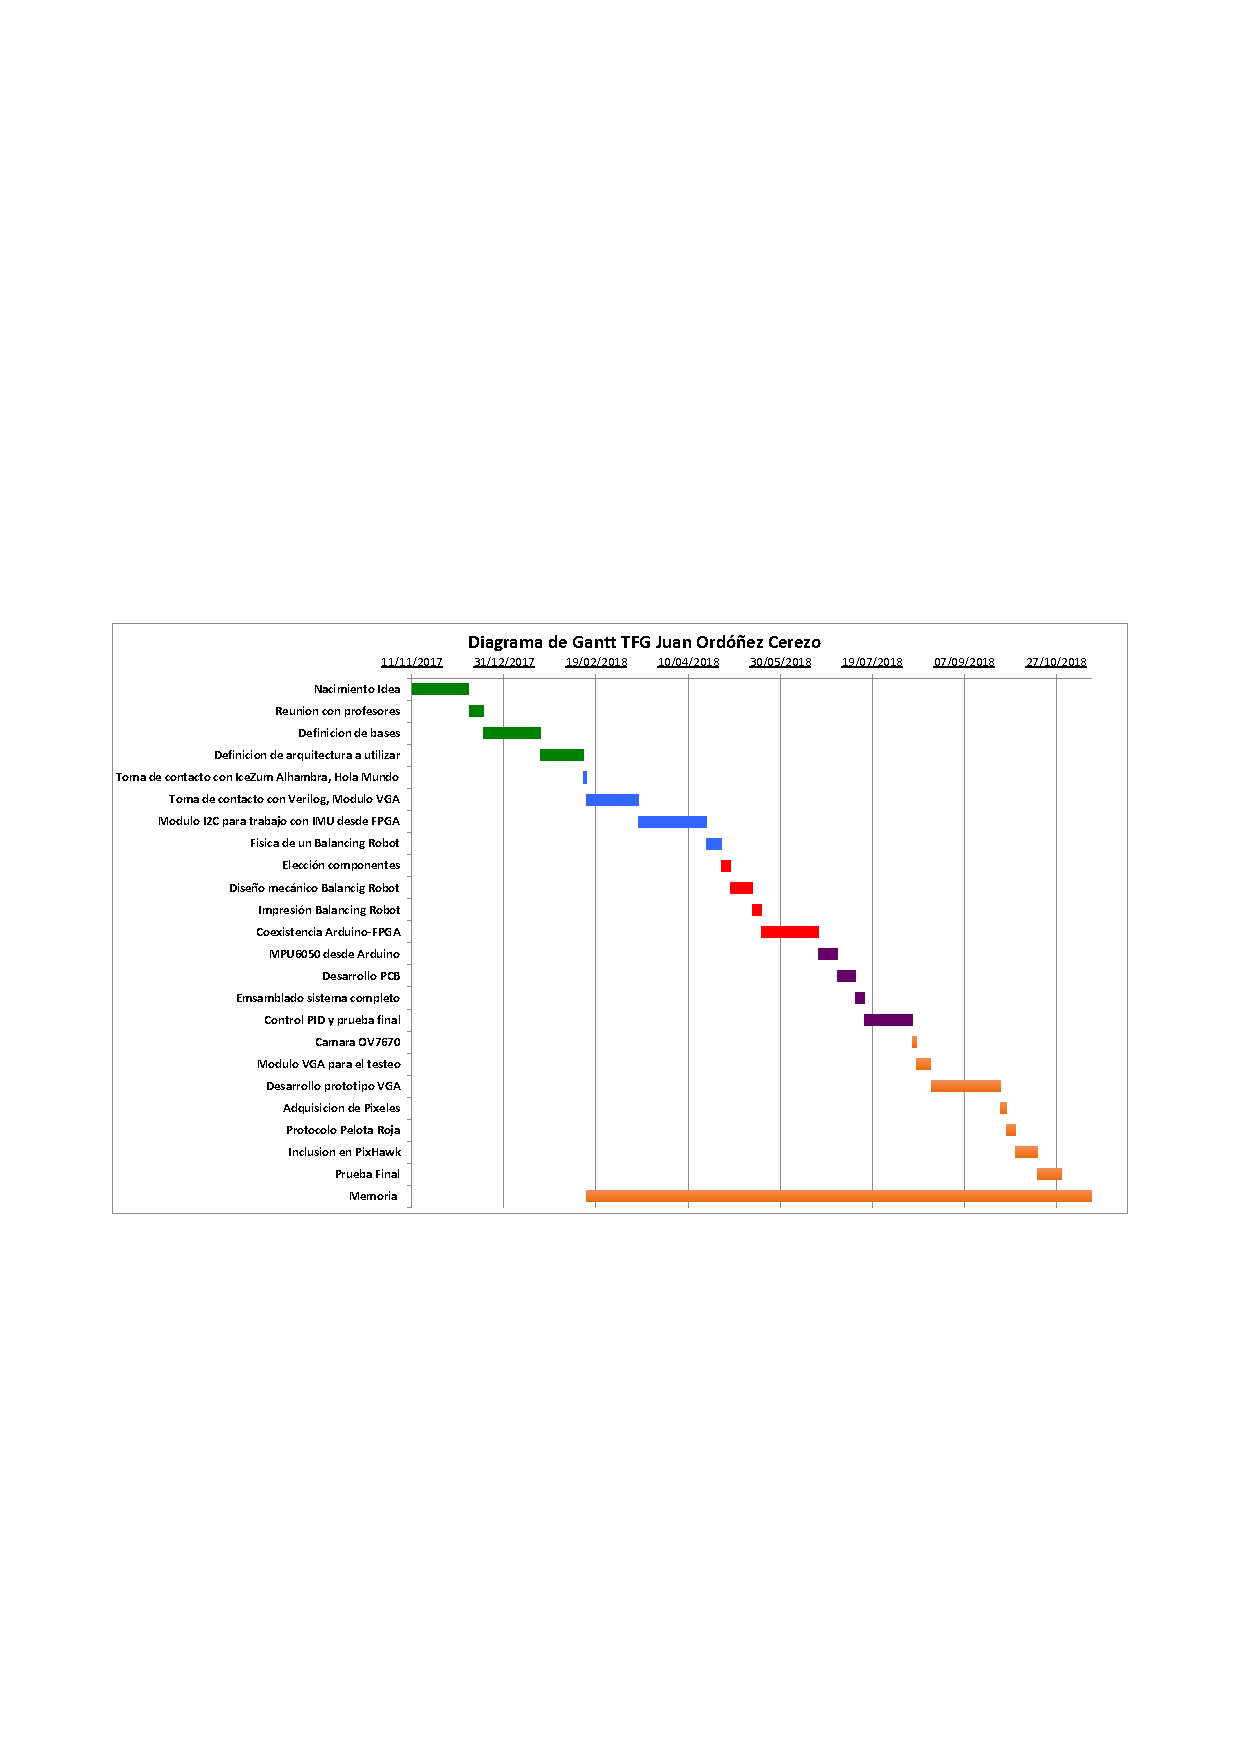
\includegraphics[trim = 15mm 85mm 0mm 100mm,clip, angle=-90, scale = 1.4]{imagenes/Introduction/Gantt.pdf}
		\label{fig:diagramaGantt}
	\end{figure}
\end{center}
\subsection{Metodología de trabajo}
Para introducir la metodología de trabajo seguida, se presenta la herramienta GitHub (figura \ref{fig:github}).\newline 

\begin{figure}[H]
	\center
	
\includegraphics[trim = 0mm 0mm 0mm 0mm, clip,scale=0.4]{imagenes/Introduction/github}
	\caption{Logo GitHub.}
	\label{fig:github}
\end{figure}


GitHub es una plataforma de desarrollo colaborativo de software para alojar proyectos utilizando el sistema de control de versiones Git. GitHub aloja tu proyecto en un repositorio y brinda herramientas muy útiles para el trabajo en equipo. \newline
Proporciona además la posibilidad de una Wiki para el mantenimiento de las versiones e información acerca de ellas. \newline
En el presente proyecto GitHub ha sido usado como un contenedor, donde se ha ido subiendo todo de manera parcial, normalmente, cuando se obtenía una versión estable sobre algunas de las ramas. \newline
De esta forma, y al ser abierto, cualquier persona ha podido seguir los avances de este, dudas, problemas, o incluso utilizar algunos de los módulos o material subidos. \newline
 
El proyecto puede encontrarse en la siguiente URL: \newline

\hyperref[]{https://github.com/RoboticsURJC-students/2017-tfg-juan-ordonez}

Un ejemplo de la trayectoria de este proyecto se representa en la captura de pantalla de GitHub en la figura \ref{fig:capturaGit}.

\begin{figure}[H]
	\center
	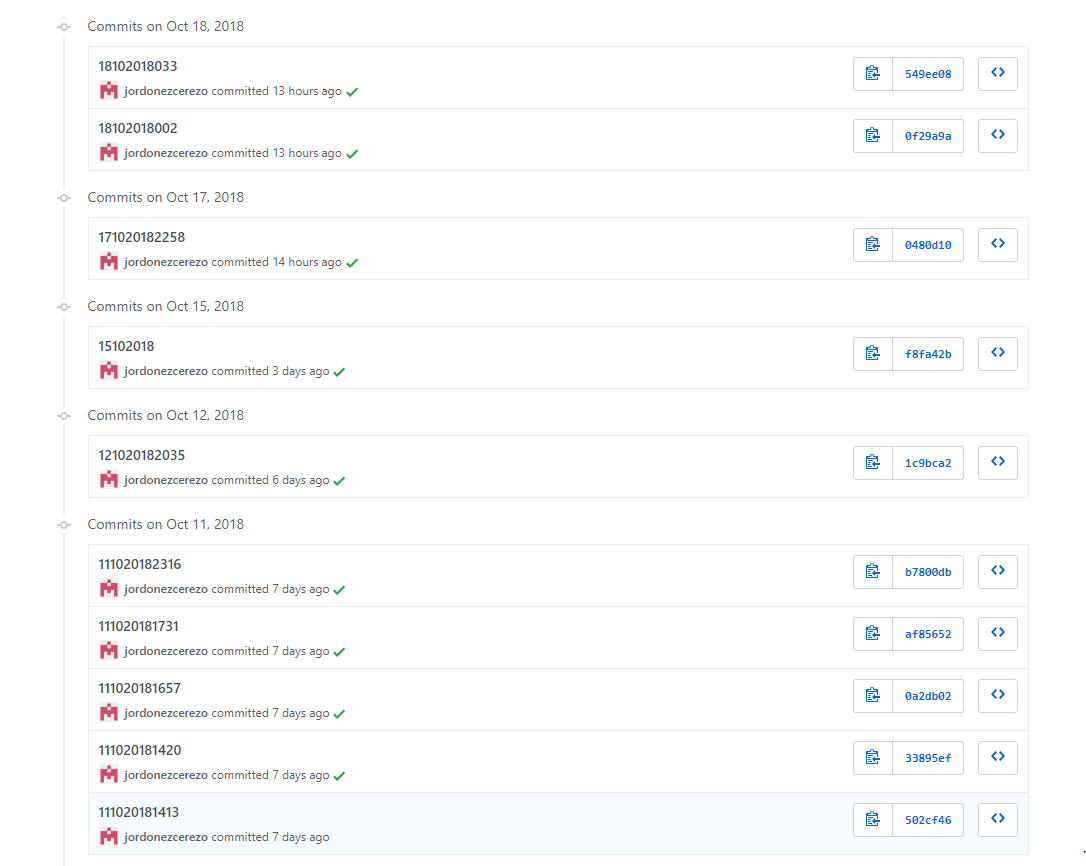
\includegraphics[trim = 0mm 0mm 0mm 0mm, clip,scale=0.5]{imagenes/Introduction/CapturaGit}
	\caption{Commits GitHub.}
	\label{fig:capturaGit}
\end{figure}

Para el buen cumplimiento de los objetivos planteados en primera instancia, y teniendo en cuenta la diferente localización de los componentes del trabajo, se hizo necesario el planteamiento de reuniones semanales (normalmente los Viernes) donde se pusiese en común lo trabajado durante la semana y se fijasen los siguientes objetivos. \newline

Para ello, se utilizo la herramienta se software libre llamada "Appear.in", la cuál ofrece videoconferencias entre varios usuarios al mismo instante (figura \ref{fig:appear}). 

\begin{figure}[H]
	\center
	
\includegraphics[trim = 0mm 0mm 0mm 0mm, clip,scale=0.3]{imagenes/Introduction/appear}
	\caption{Appear.in.}
	\label{fig:appear}
\end{figure}

\subsection{Estructura de la memoria}

La memoria está dividida en tres capítulos o partes diferenciadas. \newline
En la sección \ref{sec:Estado_arte} se explicará brevemente toda la parte teorica y conocimientos necesarios para el entendimiento del presente trabajo. Además se comentará la evolución hasta la actualidad de algunos sistemas propuestos.\newline

En la sección \ref{sec: BalancingRobot} se abordará en problema del Balancing Robot, y se diferenciara entre una parte de diseño y una parte de implementación, haciendo especial hincapié en el control PID que será utilizado en el capítulo siguiente. El Balancing Robot será capaz de mantenerse estable sobre dos ruedas horizontales.\newline

En la sección \ref{sec: Cuadricoptero} se abordará el problema de visión a bordo de un cuadricóptero. 
Una vez conseguidos los objetivos necesarios en la sección anterior, un cuadricoptero será capaz de seguir una pelota roja, por lo que se implementará el protocolo necesario para ello. \newline

Para terminar, en la sección \ref{sec: Conclusiones} se expondrán las conclusiones derivadas del trabajo completo, así como un posible trabajo futuro, errores a corregir, etc.   
%
\chapter{Estado del arte}
\section{Concepto FPGAs}
Una FPGA o (Field programmable Gate Arrays) es un dispositivo reconfigurable que puede ser eléctricamente programado para implementar una alta variedad de circuitos lógicos. Consiste en un array uniforme de estructuras lógicas programables que son interconectadas por una configurable red de enrutamiento. Un ejemplo de una red de enrutamiento puede verse en la figura \ref{fig:estructura_FPGA}

\begin{center}
	\begin{figure}[H]
		\center
		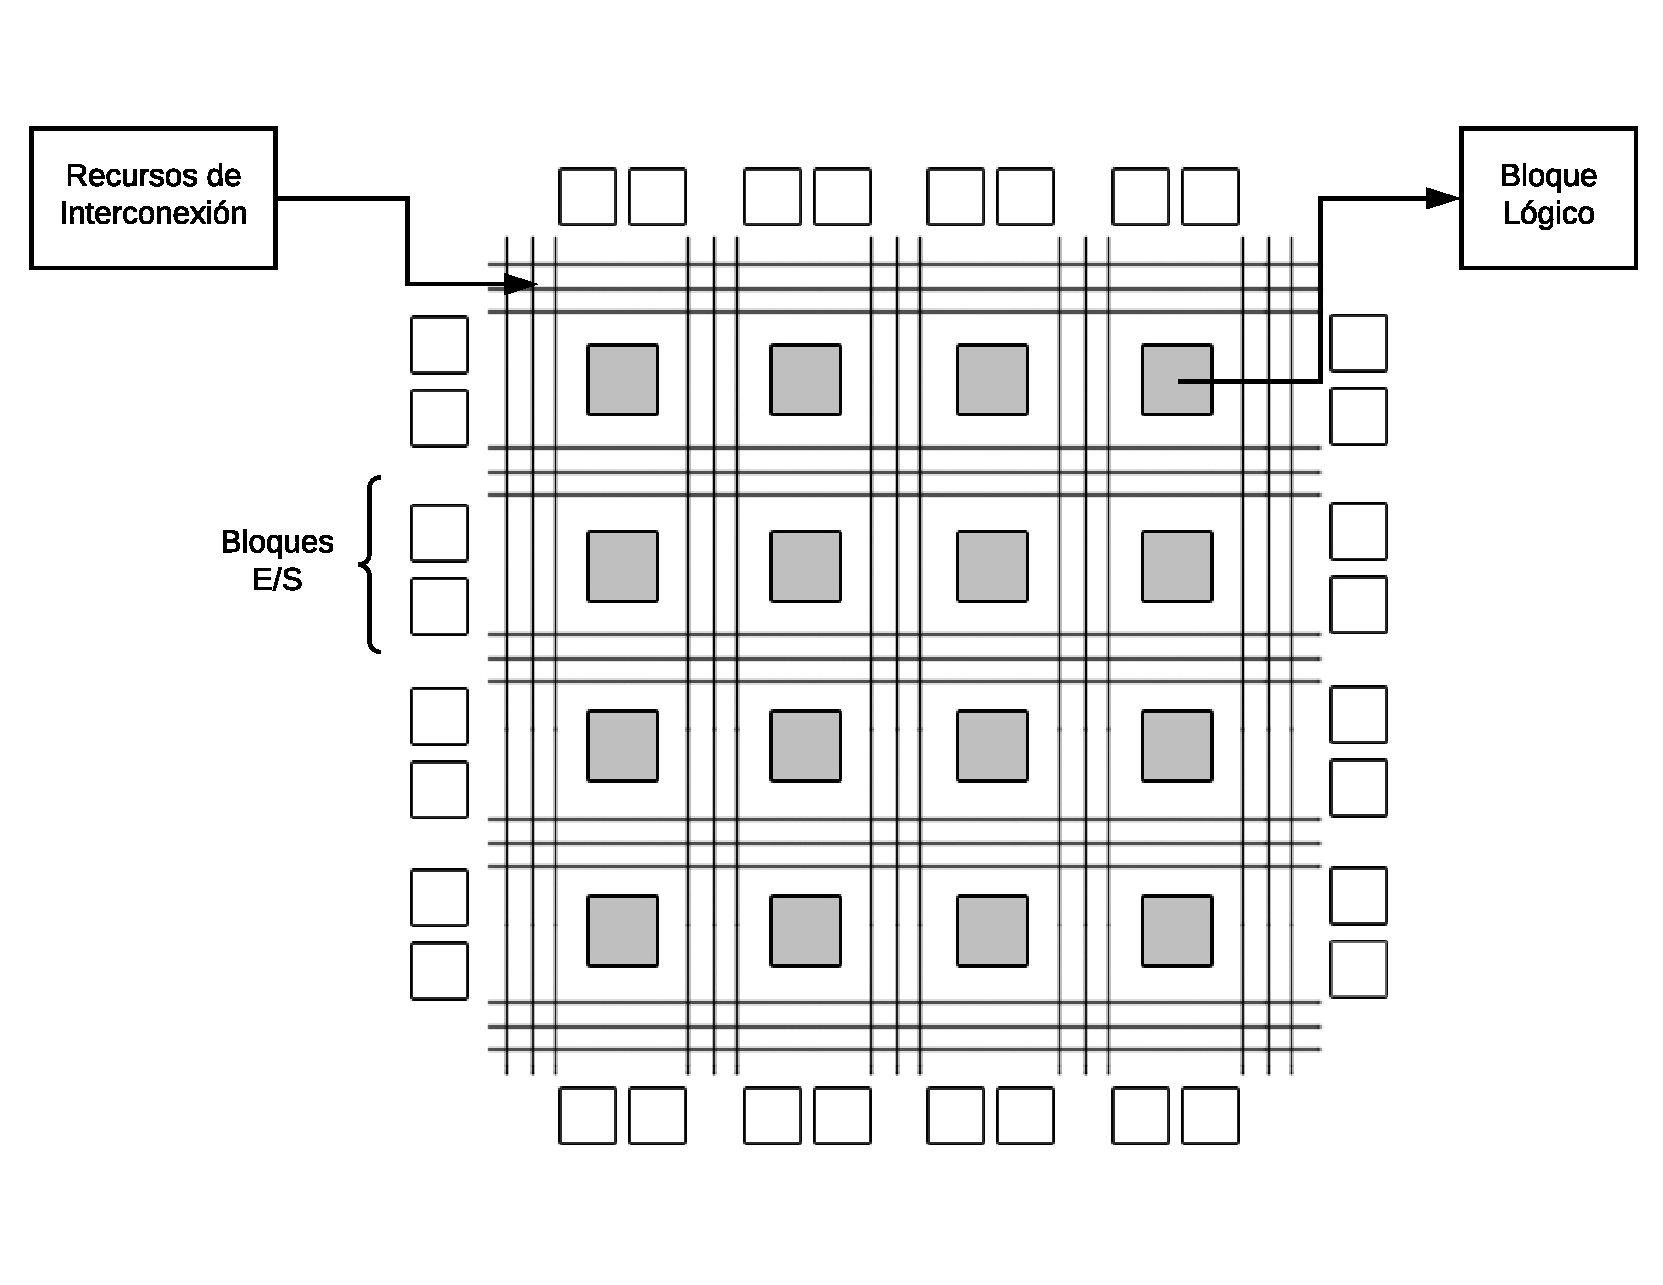
\includegraphics[trim = 0mm 10mm 0mm 10mm, clip,scale=0.4]{imagenes/EstadoArte/estructura_FPGA.pdf}
		\caption{PLD vs FPGA}
		\label{fig:estructura_FPGA}
	\end{figure}
\end{center}
 

Lo lógica y las estructuras de interconexión pueden ser configuradas gracias a potentes herramientas CAD, las cuáles permiten que el usuario final pueda definir esta interconexión física de bloques lógicos mediante lenguajes de descripción hardware (HDL). Algunos de los más conocidos son VHDL, Verilog o ABEL. 
\newline
Si bien no es el más usado actualmente, a lo largo de esta memoria se realizará una breve introducción a Verilog, comentando y analizando sus principales características.
\newpage
\subsection{Evolución y escenario}

Las FPGAs fueron inventadas en el año 1984 por Ross Freeman y Bernard Vonderschmitt, co-fundadores de Xilinx.
Originalmente fueron diseñadas para servir como prototipos o demostraciones de la funcionalidad de circuitos digitales. \newline

Las FPGAs conforman actualmente la máxima evolución de los PLDs (Programmable Logic Device), definidos estos como circuitos integrados en los que se pueden programar ecuaciones lógicas booleanas. \newline

El revolucionario éxito de estos dispositivos programables puede ser atribuido a la flexibilidad en la implementación del diseño. Así, la capacidad de re-programar al instante la FPGA con varios circuitos sin costo adicional, promueve la re-utilización del dispositivo, permite una rápida verificación del diseño y por ello, reduce el gasto en la etapa de desarrollo. \newline

Si bien actualmente no representan todo el sistema de un producto final, sus ventajas en las propiedades del diseño hacen que estén empezando a formar parte de una pieza importante en el desarrollo de un producto electrónico. \newline

Para intentar entender el porqué de la importancia de dispositivos de implementación hardware sería adecuado introducir la Ley de Moore. \newline 
La ley de Moore expresa que aproximadamente cada dos años se duplica el número de transistores en un microprocesador. Como se puede ver en la figura \ref{fig:Ley_de_Moore}, esta ley que formuló el cofundador de Intel E. Moore el 19 de Abril de 1965 no se aleja de la realidad: 
\newline
\begin{figure}[H]
	\center
	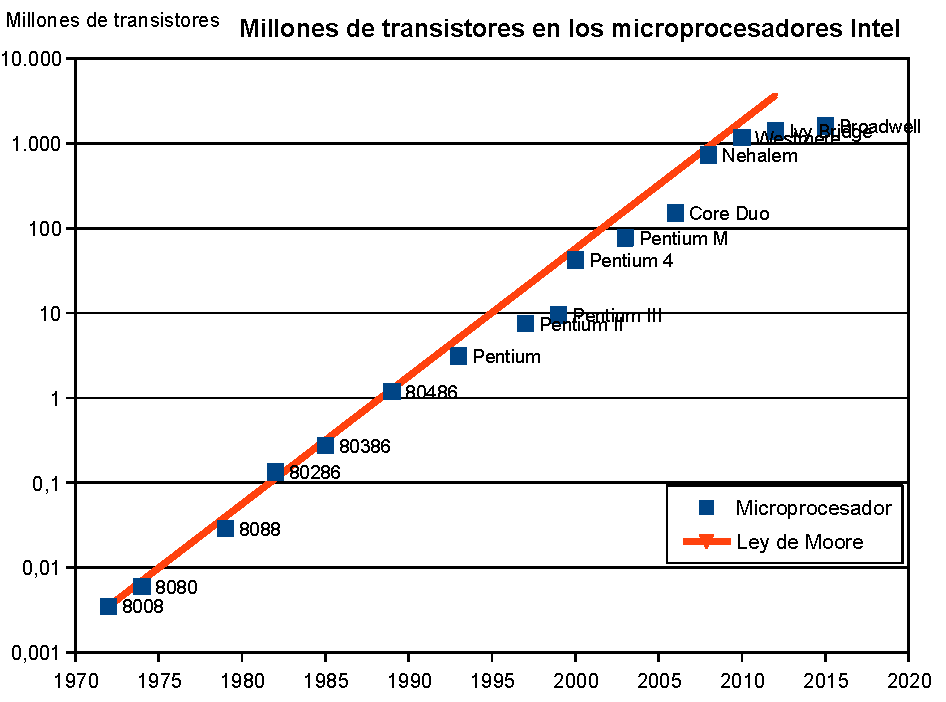
\includegraphics[scale=0.7]{imagenes/EstadoArte/ley_moore-eps-converted-to.pdf}
	\caption{Ley de Moore}
	\label{fig:Ley_de_Moore}
\end{figure}
 

No obstante, tal y como ya han anunciado las principales empresas de microprocesadores actuales como son Intel y AMD en su hoja de ruta tecnológica para semiconductores, la ley de Moore llegará a su fin en 2021. \newline

Después de esa fecha, no resultará económicamente eficiente reducir más el tamaño de los transistores de silicio. La predicción de la industria no es que simplemente su tasa de reducción será cada vez más lenta, sino que se va a detener definitivamente. \newline

Es aquí donde la electrónica digital comenzará a tener un papel importante en los microprocesadores. Tanto es así que multinacionales dedicadas a la fabricación de procesadores como pueden ser Intel o AMD ya están trabajando en implementar esos comportamientos en FPGAs. Sus ventajas e inconvenientes serán presentadas en el los capítulos \ref{sec:ArquitecturaFPGA} y \ref{sec:DescripcionHardware}.

\subsection{Arquitectura FPGA}\label{sec:ArquitecturaFPGA}

En un PLD, las interconexiones entre elementos ya esta prefijada, y solo es posible habilitar o deshabilitar esta conexión. \newline
Por el contrario, sobre FPGA estas interconexiones no están prefijadas, siendo el usuario final el que decide las interconexiones entre bloques lógicos:
\newline
\begin{center}
\begin{figure}[H]
	\center
	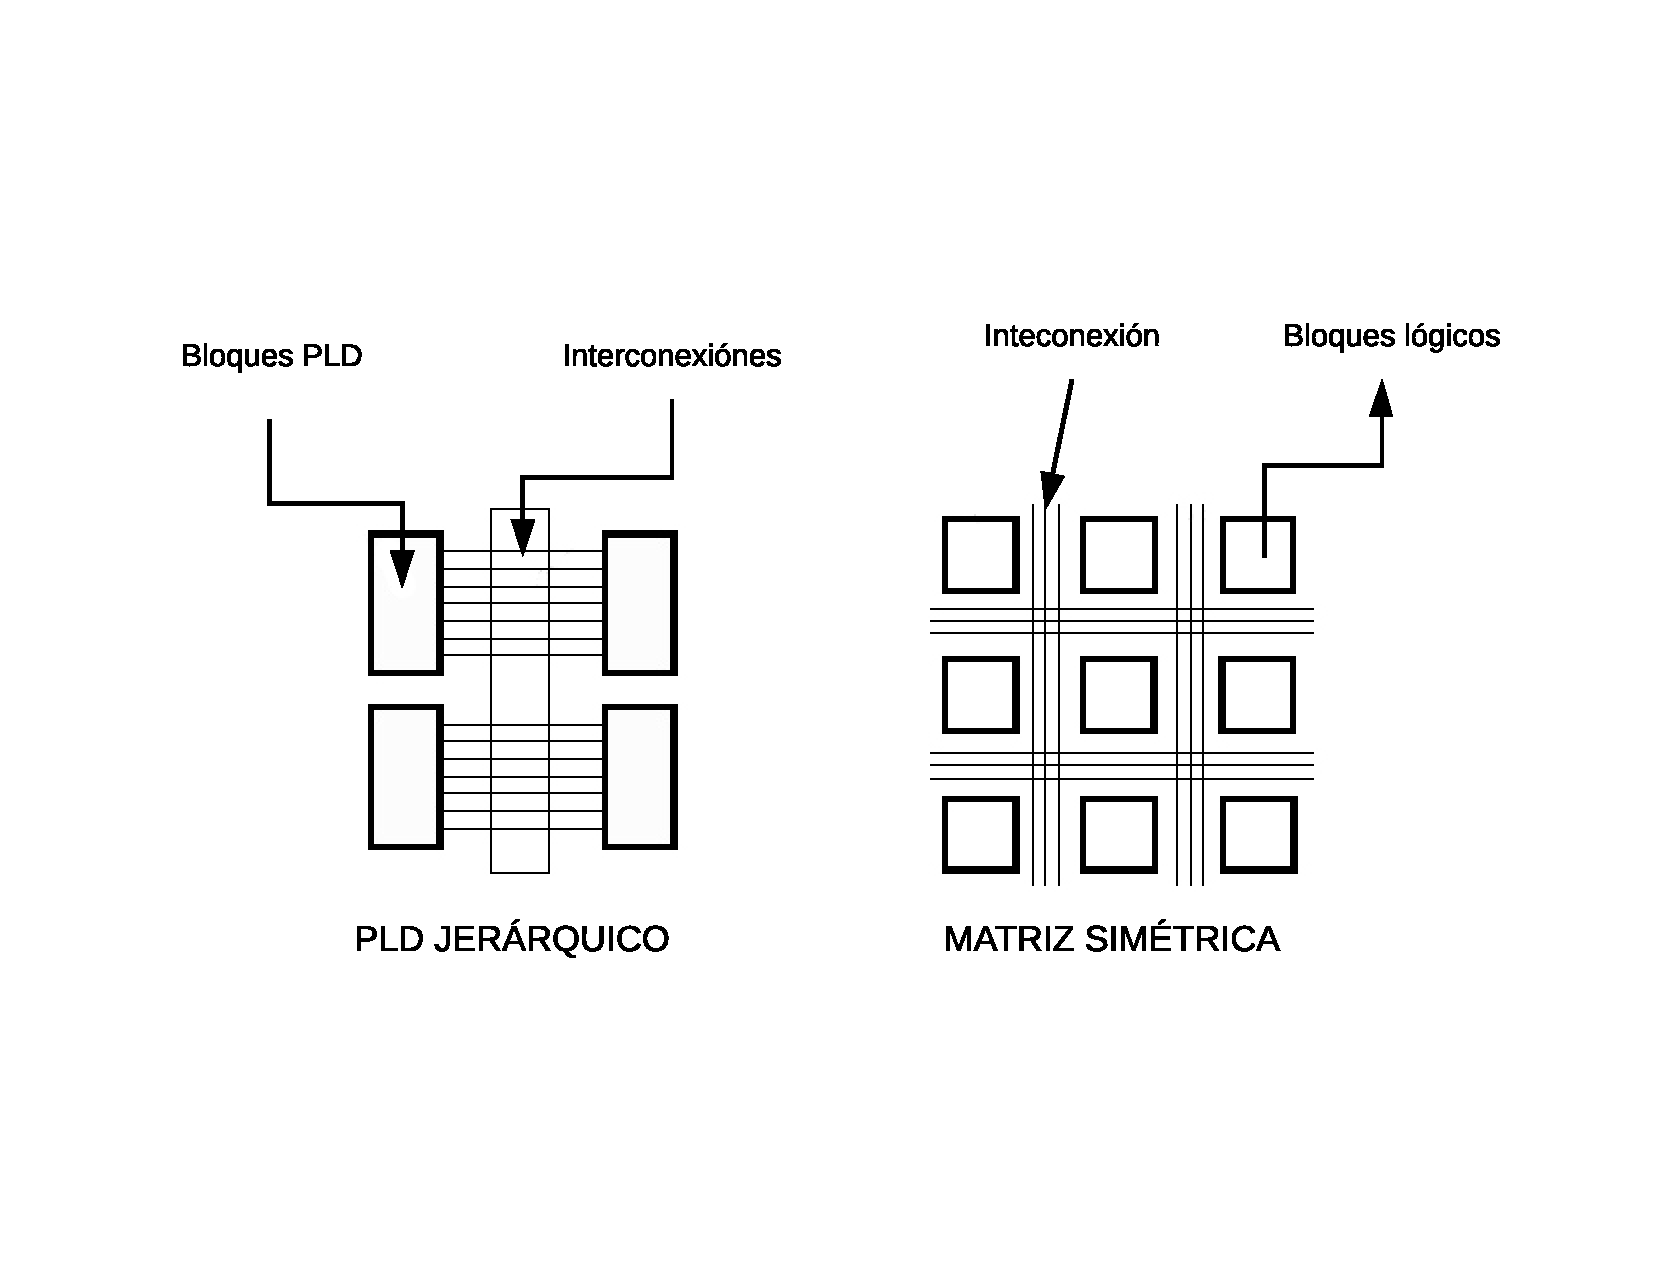
\includegraphics[trim = 10mm 35mm 10mm 35mm, clip,scale=0.6]{imagenes/EstadoArte/pld_fpga.pdf}
	\caption{PLD vs FPGA}
	\label{fig:pld_fpga}
\end{figure}

\end{center}

A la hora de elegir una FPGA para un proyecto determinado es importante tener en cuenta una de sus propiedades más importantes, el número de bloques lógicos. \newline
El número de bloques lógicos determinan la capacidad del dispositivo y forma parte de una de las características mas limitantes de las FPGAS en la actualidad. Los bloques lógicos son independientes entre sí y pueden interconectarse para formar un módulo más complejos. \newline

A continuación se introducirán los conceptos de granularidad fina y granularidad gruesa, que dará lugar al correcto entendimiento de la arquitectura en una FPGA. 

Estos módulos más complejos realizan las operaciones básicas que en conjunto representan la función que operará en una FPGA. Se dice que la FPGA son dispositivos con una arquitectura avanzada por la densidad de sus componentes y por los diferentes caminos de interconexión entre módulos. Así, de acuerdo al tipo de módulos lógicos que la conforman, encontramos dos derivaciones estructurales: 
\begin{itemize}
	\item Granularidad Gruesa.
	\item Granularidad Fina.
\end{itemize}

Los módulos lógicos en una arquitectura de granularidad gruesa son módulos grandes generalmente consistentes de una o más tablas de búsqueda y dos o más flip-flops. La tabla de búsqueda, también conocida como LookUp Table (LUT), actúa como una memoria donde se encuentra almacenada la tabla de verdad que representa la función lógica del circuito, así, en una LUT se puede implementar cualquier función deseable.\newline

Por otra parte, una arquitectura de granularidad fina, está estructurada por una gran cantidad de módulos lógicos pequeños que realizan funciones relativamente simples. Cada módulo está compuesto de un circuito de dos entradas que realiza una función lógica determinada, o en algunos otros casos por un multiplexor. También suele contener algún flip-flop.  \newline

La FPGAs mas utilizadas actualmente suelen contar con tecnología de granularidad gruesa, que permite elevar el nivel de abstracción con respecto a las FPGA de granularidad fina. \newline

El primer caso permite implementaciones menos detalladas ya que desde un nivel muy básico se tienen módulos más complejos y el hecho de utilizar LUT deja entrever que se pueden realizar diseños más grandes. A lo largo de este proyecto se trabajará con el primer caso, ejemplo de ello es la FPGA utilizada, IceZum Alhambra II. \newline

El diseñador propone la función lógica a realizar a través de métodos de descripción hardware y define los parámetros de su problema. Esto se hace por medio de código programable, que puede ser un lenguaje de descripción hardware, los cuáles son introducidos en el capítulo \ref{sec:DescripcionHardware}. 

\subsection{Lenguajes de descripción hardware}\label{sec:DescripcionHardware}

Un HDL(Hardware Description Languaje) es un lenguaje usado para modelar el funcionamiento de un bloque hardware en una forma textual. \newline 
Al igual que podemos encontrar diferencias entre los diferentes tipos de lenguajes de programación en cuanto a su sintaxis de codificación y sus métodos de simulación y síntesis, se observan ciertas diferencias entre HDL's. \newline
Se tienen dos tipos diferentes de lenguajes de descripción hardware:
\begin{itemize}
	\item Bajo modelado. No permiten la jerarquezación de módulos y son capaces de realizar solo descripciones simples.
	\item Alto modelado. Son los mas utilizados actualmente, permiten diseñar sistemas más complejos. Ejemplos de alto modelado son Verilog (Verify Logic) y VHDL (VHSIC Hardware Description Language).
\end{itemize}	
Este trabajo se basará en Verilog por permitir un nivel más alto de implementación que VHDL, como será analizado en la sección \ref{sec:Verilog} . \newline

Ambos lenguajes comparten algunas características comunes, como el soporte para cualquier nivel de modelado y abstracción, y que cada elemento de diseño tiene una interfaz bien definida, para permitir la conexión rápida con otros elementos lógicos.

\subsection{Verilog}\label{sec:Verilog}
Debido a su utilización a lo largo de este proyecto, se analizarán algunas características importantes cuyo conocimiento será básico para entender el código.

\subsubsection{Tipos de datos}

Existen dos tipos de datos en Verilog los cuáles tienen que ser entendidos para poder alcanzar la funcionalidad buscada:
\begin{itemize}
	\item reg: Representan variables con capacidad para almacenar información.
	\item wire: Representan conexiones entre componentes, no tienen capacidad de almacenamiento.
\end{itemize}

\subsubsection{Implementación en módulos}
En la mayoría de los casos y para no perder el nivel de abstracción, un proyecto en Verilog suele estar compuesto por un conjunto de módulos los cuáles forman una funcionalidad completa, y cada uno de ellos, una especifica. \newline

Las características principales de la implementación digital por módulos son:
\begin{itemize}
	\item Cada módulo dispone de una serie de entradas y salidas cuya función principal es interconectar otros módulos, aunque puede no tener entradas y salidas.
	\item No existen variables globales.
	\item Cada módulo puede describirse de forma arquitectural o de comportamiento.
\end{itemize}

Esta implementación por módulos Verilog permite la configuración del nivel de abstracción deseado por el usuario final. \newline
El desarrollo de módulos de funcionalidad específica puede tener sus ventajas e inconvenientes dependiendo de su uso final. \newline
Si se quieren reutilizar para otros flujos de trabajo (ejemplo: sumador 8 bits), es bueno tener módulos muy definidos según su funcionalidad (ejemplo: sumador de 2 bits). Sin embargo, la polarización no tiene porque ser imprescindible, si bien aconsejada.

\subsubsection{Paralelización de Procesos}
Una de las características mas importantes que diferencia a Verilog del resto de lenguajes procedurales es la posibilidad de ejecutar varios procesos en paralelo, aspecto fundamental en el lenguaje, y el cuál le brinda gran parte de las ventajas de usar implementación hardware.

\begin{center}
	\begin{figure}[H]
		\center
		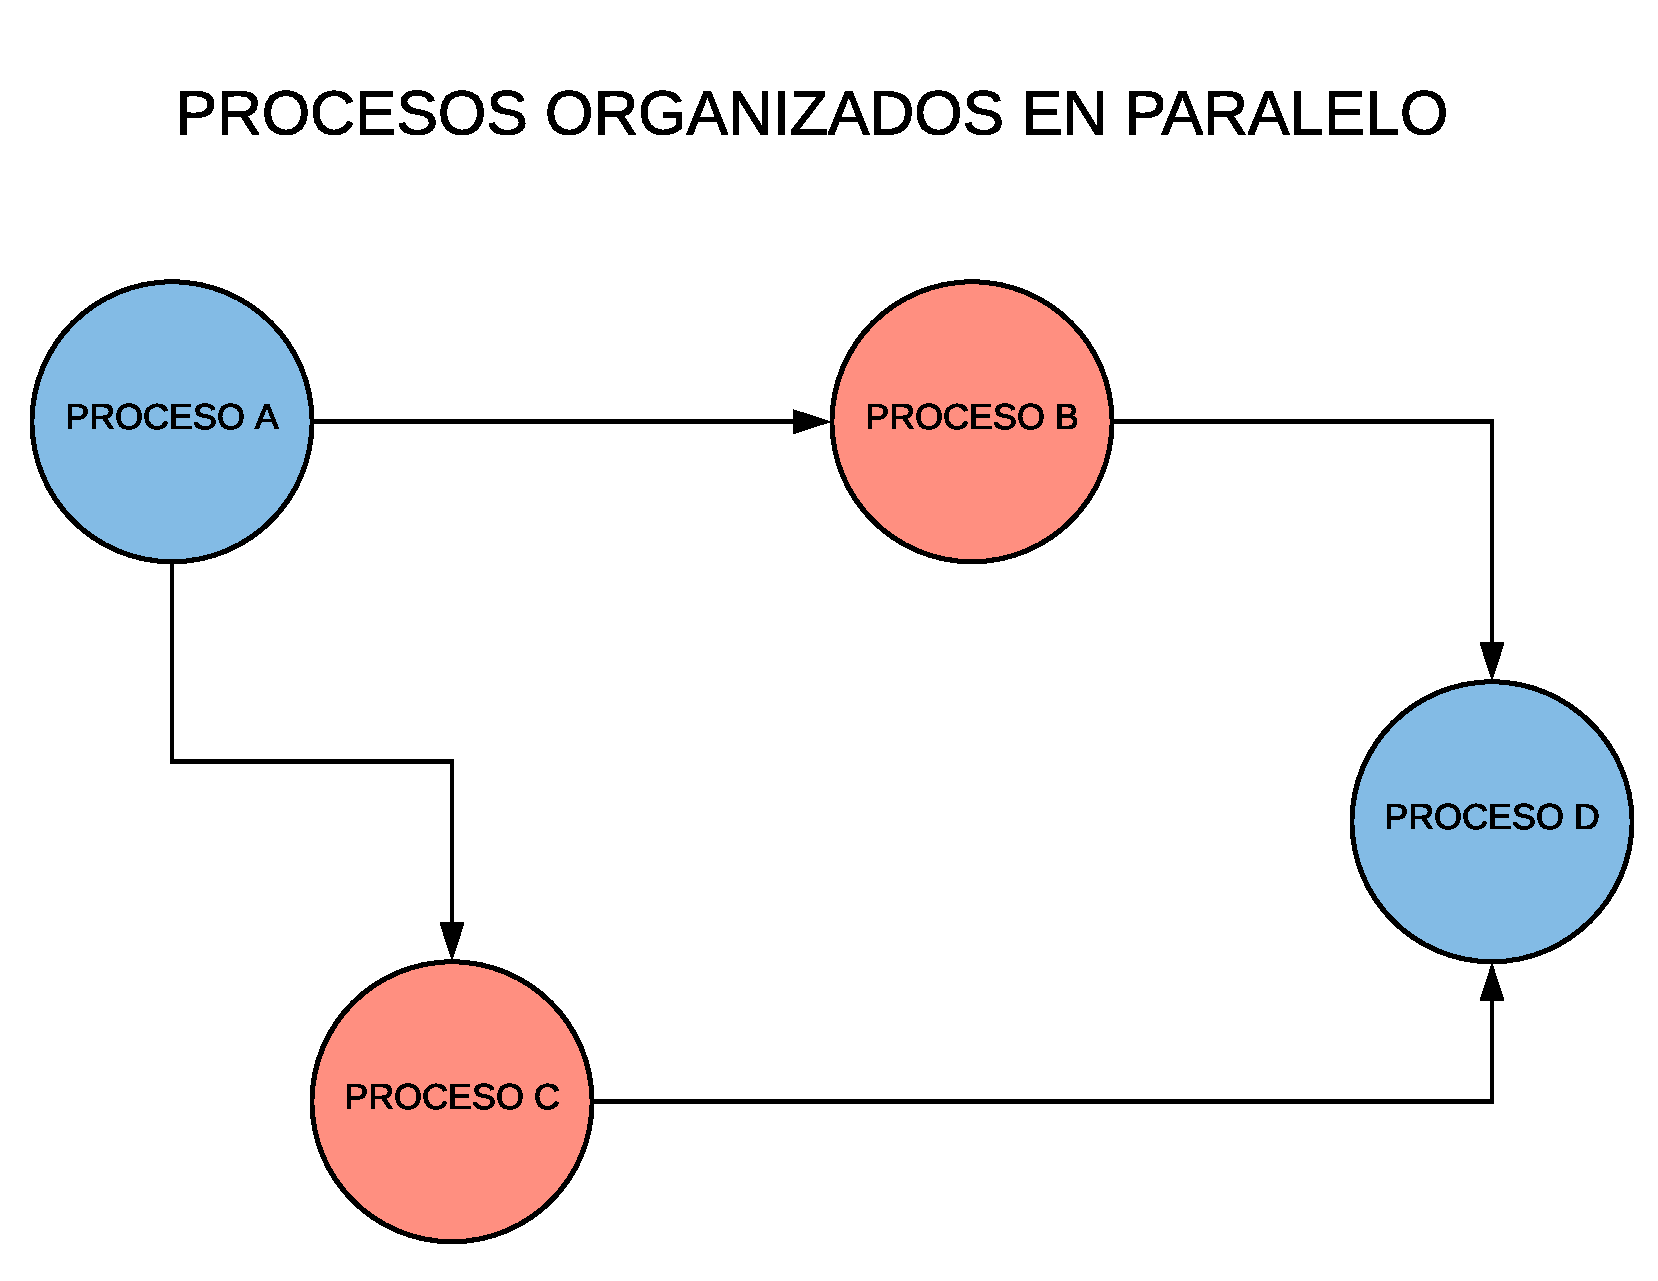
\includegraphics[trim = 0mm 0mm 0mm 0mm, clip,scale=0.3]{imagenes/EstadoArte/procesos_paralelo.pdf}
		\caption{Paralelización de Procesos}
		\label{fig:procesos_paralelo}
	\end{figure}
	
\end{center}
Toda la descripción del comportamiento en Verilog debe declarase dentro de un proceso, estos pueden ser dos tipos:

\begin{itemize}
		\item Initial: Este tipo de procesos se ejecutan sólo una vez comenzando su ejecución al inicio, y por tanto no existen retardos. Este proceso no es sintetizable, es decir, no puede ser utilizado en una descripción RTL.
		
		\item Always: Este tipo de procesos se ejecuta continuamente a modo de bucle, y como su propio nombre indica, está continuamente ejecutándose. Este proceso si que es sintetizable y es controlado por la temporización o por eventos. Si dicho bloque se ejecuta por más de un evento, dicho conjunto se denomina lista sensible.
\end{itemize}

\subsubsection{Estructuras de control}

Al igual que los leguajes de tipo procedural, Verilog dispone de una serie de estructuras de control:

\begin{itemize}
	\item if - else
	\item Case. Es una de las estructuras de control mas utilizadas a lo largo de este proyecto, permite la generación de máquinas de estados
	\item For
	\item While
	\item Forever
	\item Wait
	
\end{itemize}

\subsubsection{Asignación continua}

Mediante la asignación continua se puede modelar lógica combinacional, es decir, mo se necesita una lista de sensibilidad para realizar la asignación. Sólo puede ser declarada fuera de cualquier proceso.

\subsubsection{Asignación procedural}

A las variables se le asigna un valor dentro de un proceso always o initial, el tipo de variable a la que se le asigna el valor puede ser de cualquier tipo.

%%%%%%%%%%%%%%%%%%%%%%%%%%%%%%%%%%%%%%%%%%%%%%%%%%

\section{FPGAs libres}
\subsection{Evolución}
\subsection{Escenario}
\subsection{IceZum Alhambra}
Para este trabajo se ha optado por trabajar con la IceZum Alhambra, la cuál ha sido íntegramente diseñada y ensamblada en España.\newline
Es una FPGA libre y compatible con IceStudio (el cuál se verá a continuación). Alguna de sus características más importantes pueden ser:
\begin{itemize}
	\item Placa FPGA de desarrollo iCE40HX1K-TQ144 de la empresa Lattice. 
	\item Open hardware.
	\item Compatible con IceStorm toolchain.
	\item Compatible con shields de Arduino Uno. 
	\item 12MHz Oscilador.
	\item Interuptor ON/OFF para activar o desactivar los pines digitales.
	\item 20 Input/output 5v pines.
	\item 8 Input/Output 3.3V pines
	\item USB micro-B para programar la FPGA desde el pc.
	\item Botón de reset.
	\item 8 leds de proposito general.
	\item TX/RX Leds
	\item 4 entradas analógicas disponibles a través de i2c.
\end{itemize}

Es conocido que existen placas con mejores carácterísticas, pero el hecho de que sea Open Hardware y que se pueda implementar con IceStudio, ha llevado a la elección final de esta placa para el desarrollo del presente proyecto.\newline
\begin{center}
\begin{figure}[H]
	\center
	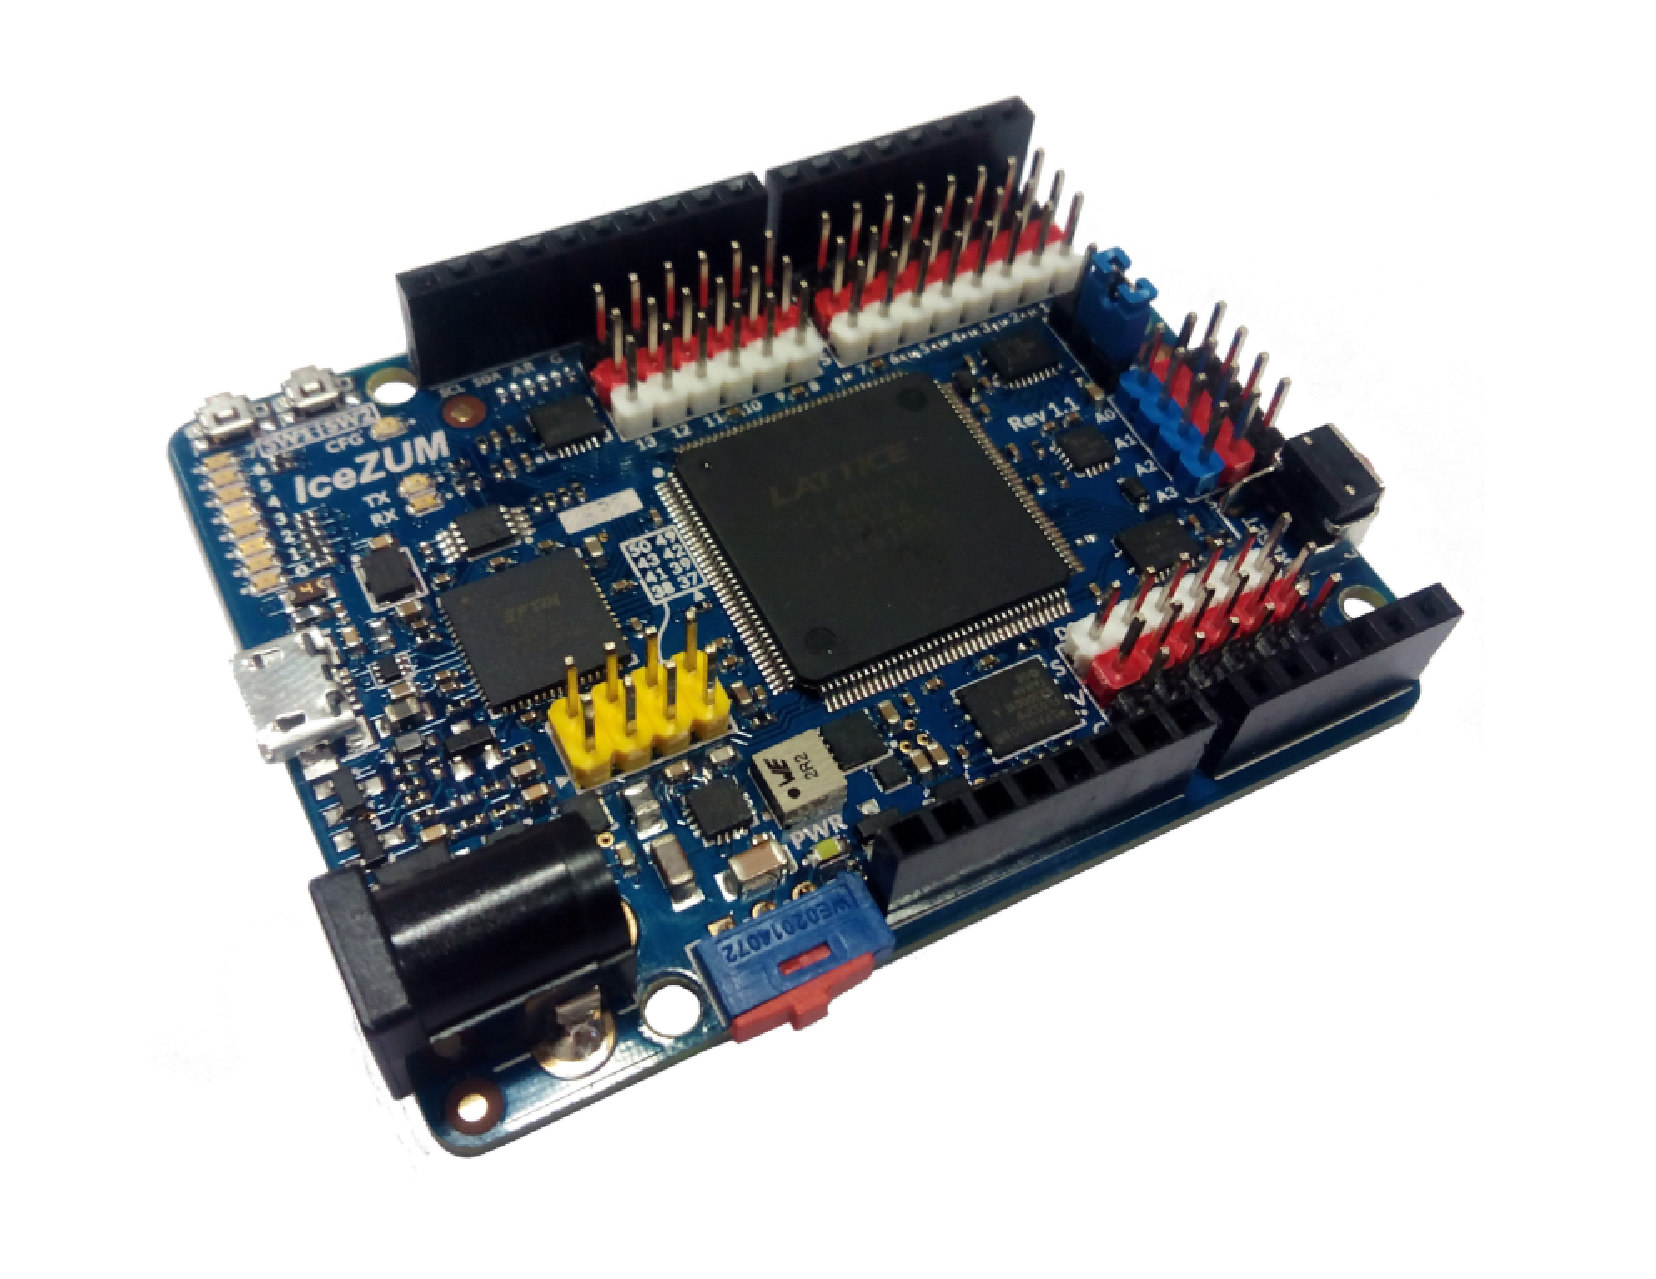
\includegraphics[scale=0.4]{imagenes/EstadoArte/IceZumAlhambra.pdf}
	\caption{IceZum Alhambra Board}
	\label{fig:IceZumAlhambraI}
\end{figure} 
\end{center}
Un punto a tener en cuenta para el desarrollo de hardware con esta FPGA es su limitada memoria de 1K lo que ha supuesto una limitación importante en el desarrollo. Es por ello que también se utilizado para el presetne proyecto la nueva versión de la IceZum Alhambra, IceZum Alhambra II, la cuál aún no estaba en el mercado al inicio del proyecto y que conlleva algunas mejoras, como la ampliación de 8K en su memoria, la mejora del bus de datos i2c, la posibilidad de alimentación mediante batería LIPO, etc. \newline
La IceZum Alhambra II es la representada en la figura \ref{fig: IceZumAlhambraII}
\begin{center}
	\begin{figure}[H]
		\center
		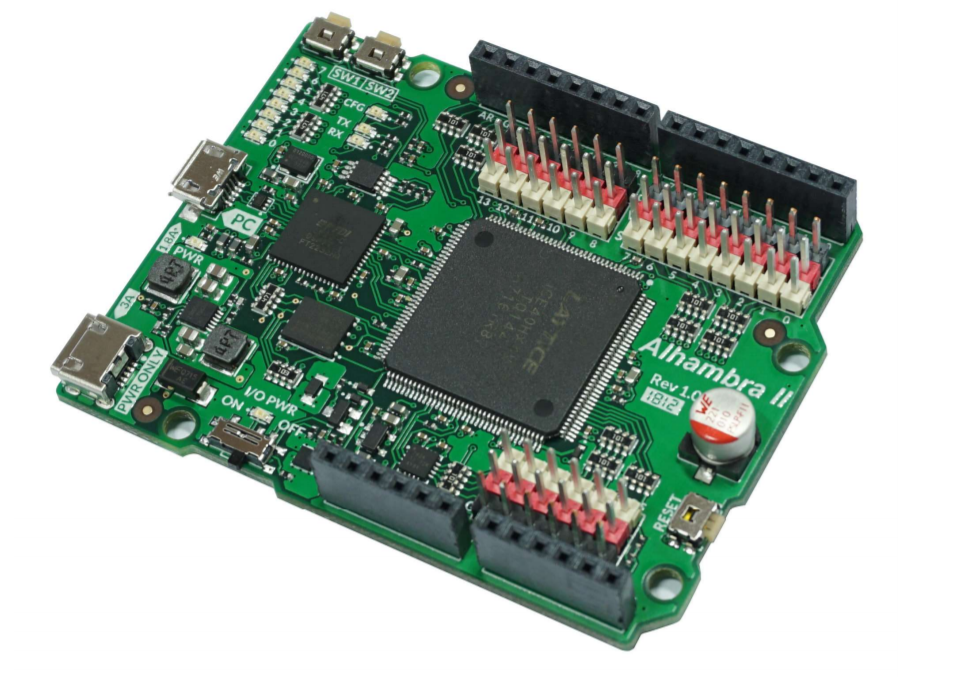
\includegraphics[scale=0.5]{imagenes/EstadoArte/IceZumAlhambra.PNG}
		\caption{IceZum Alhambra II Board}
		\label{fig: IceZumAlhambraII}
	\end{figure} 
\end{center}


\subsection{IceStudio}
Los lenguajes HDL suelen tener una curva de aprendizaje difícil, debido esto en gran medida al nivel de abstracción tan bajo necesario para diseñar un sistema en concreto. Es necesario conocer las características hardware de nuestro sistema para poder trabajar con este tipo de lógica. \newline

Como se ha desarrollado anteriormente, algunos fabricantes proporcionan herramientas comerciales para programar sus propios FPGA. Si bien en la actualidad son entornos complejos, cuentan con una gran cantidad de herramientas y funcionalidades. Lamentablemente la mayoría de ellos no son gratuitos y están unidos a la arquitectura de un único fabricante.
\newline
Con la evolución de las FPGAs han empezado a aparecer lenguajes que permiten un mayor nivel de abstracción. 
Además, también han aparecido herramientas centradas en la implementación gráfica. Un ejemplo de este tipo de implementación es LabVIEW FPGA o IceStudio. \newline
IceStudio es un proyecto Open Source desarrollado por Jesús Arroyo Torrens y sobre el que nos basaremos a lo largo del presente documento. \newline

IceStudio es IDE gráfico para FPGAs libres y esta construido sobre el proyecto IceStorm. 
El proyecto IceStorm tiene como objetivo la ingenieria inversa y la documentación del formato bitstream de la FPGA Lattice iCE40 (aunque más adelante fueron surgiendo algunas más). Proporciona herramientas simples para analizar y crear archivos de flujo de bits, esto es, el más bajo de nivel de implementación para una FPGA.\newline

Para acercar al lector al conocimiento y funcionamiento de IceStudio se irán incorporando a lo largo del documento una serie de capturas de pantalla representativas para que no se pierda la visión de lo que se esta haciendo. Por ejemplo, la ventana principal de IceStudio y sobre la que se desarrollará todo lo demás tendrá la siguiente apariencia: \newline

\begin{figure}[H]
	\center
	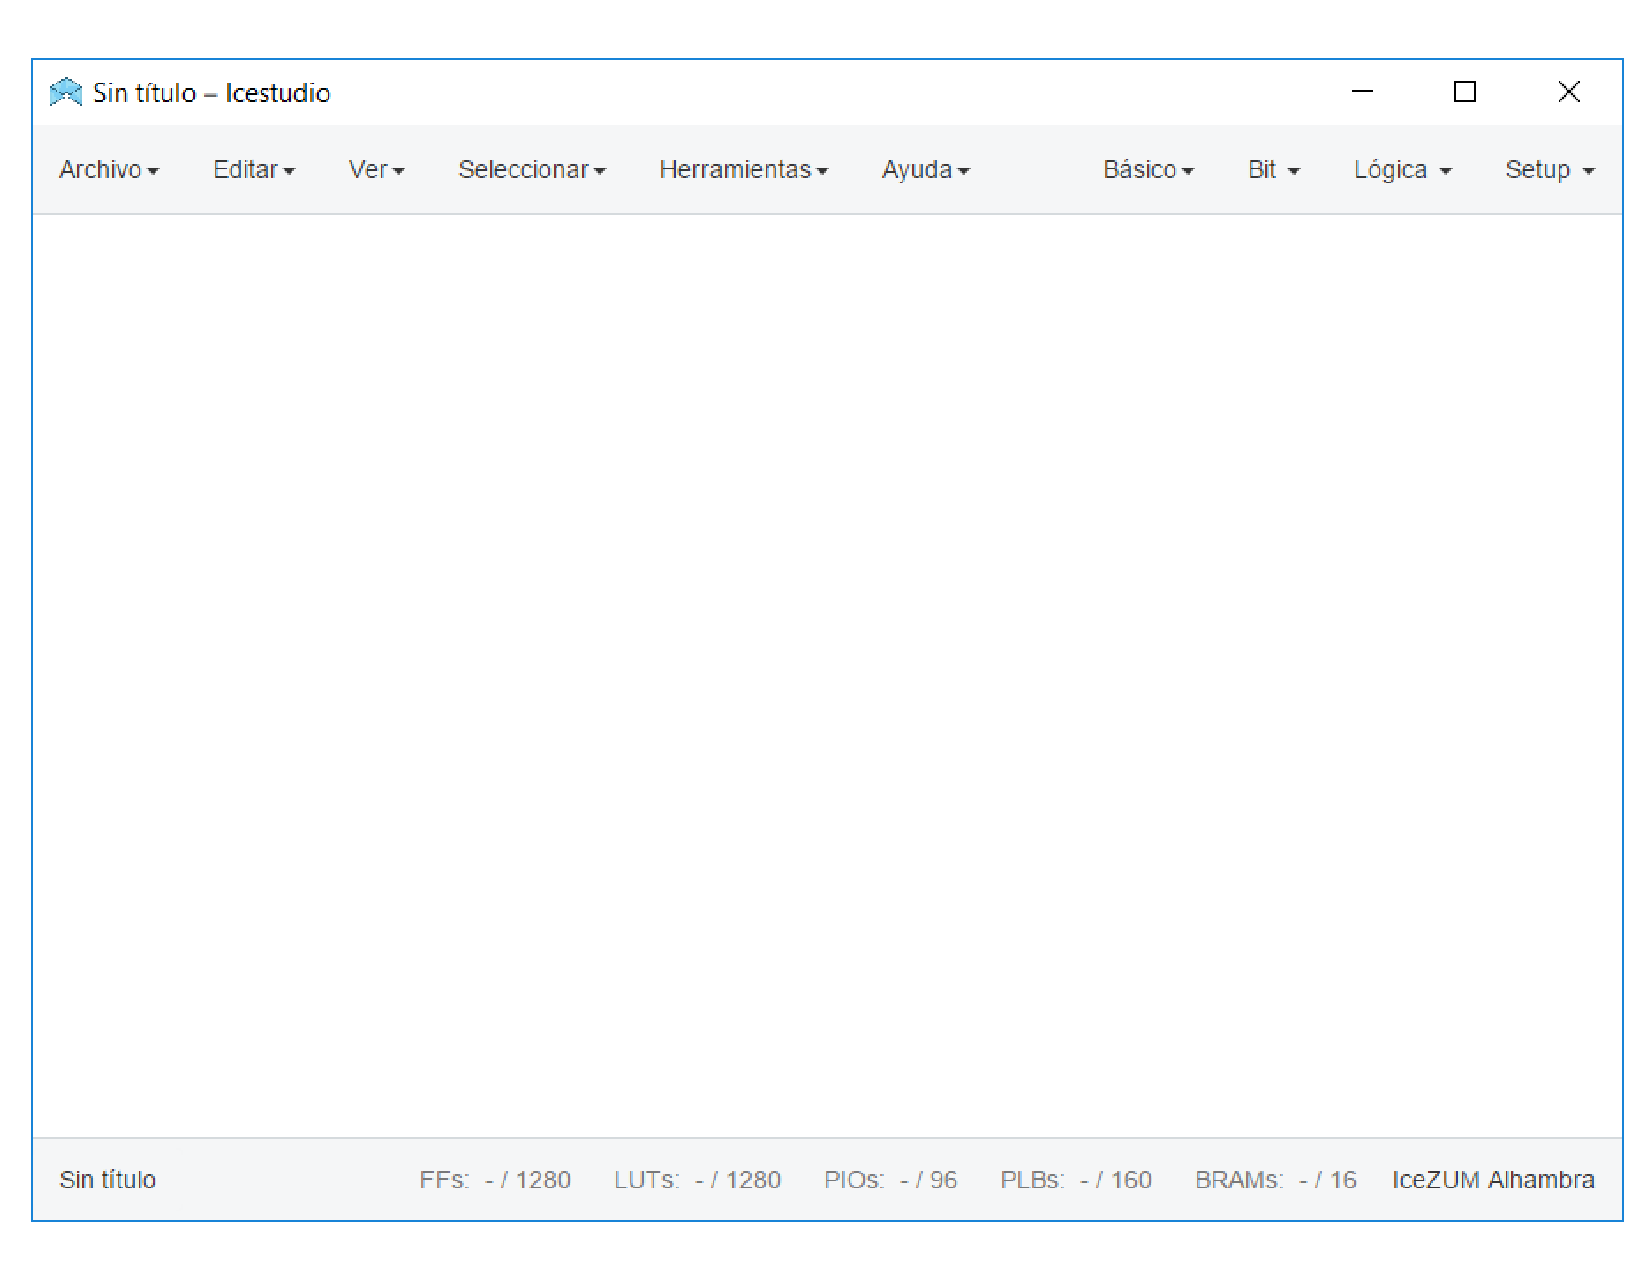
\includegraphics[trim = 0mm 0mm 0mm 0mm, clip,scale=0.4]{imagenes/EstadoArte/Main_IceStudio.pdf}
	\caption{Ventana principal IceStudio.}
	\label{fig:Main_IceStudio}
\end{figure}

El hecho de que IceStudio sea un editor gráfico puede hacer pensar que el nivel de abstracción podría ser más alto de lo deseado, pero lo cierto es que este nivel es configurable. \newline
Es el usuario final el que decide con que nivel de abstracción se trabaja, siendo necesario para eso una amplia biblioteca de módulos como veremos a continuación. Para poder explicar la potencia de IceStudio, se procederá con un ejemplo;\newline

El módulo que se presenta en la imagen \ref{fig:Write_i2c_module} es una escritura normal de i2c, en la cuál se parametriza la dirección del esclavo y la dirección que se quiere leer (más adelante se explicará con más detalle). \newline

\begin{figure}[H]
	\center
	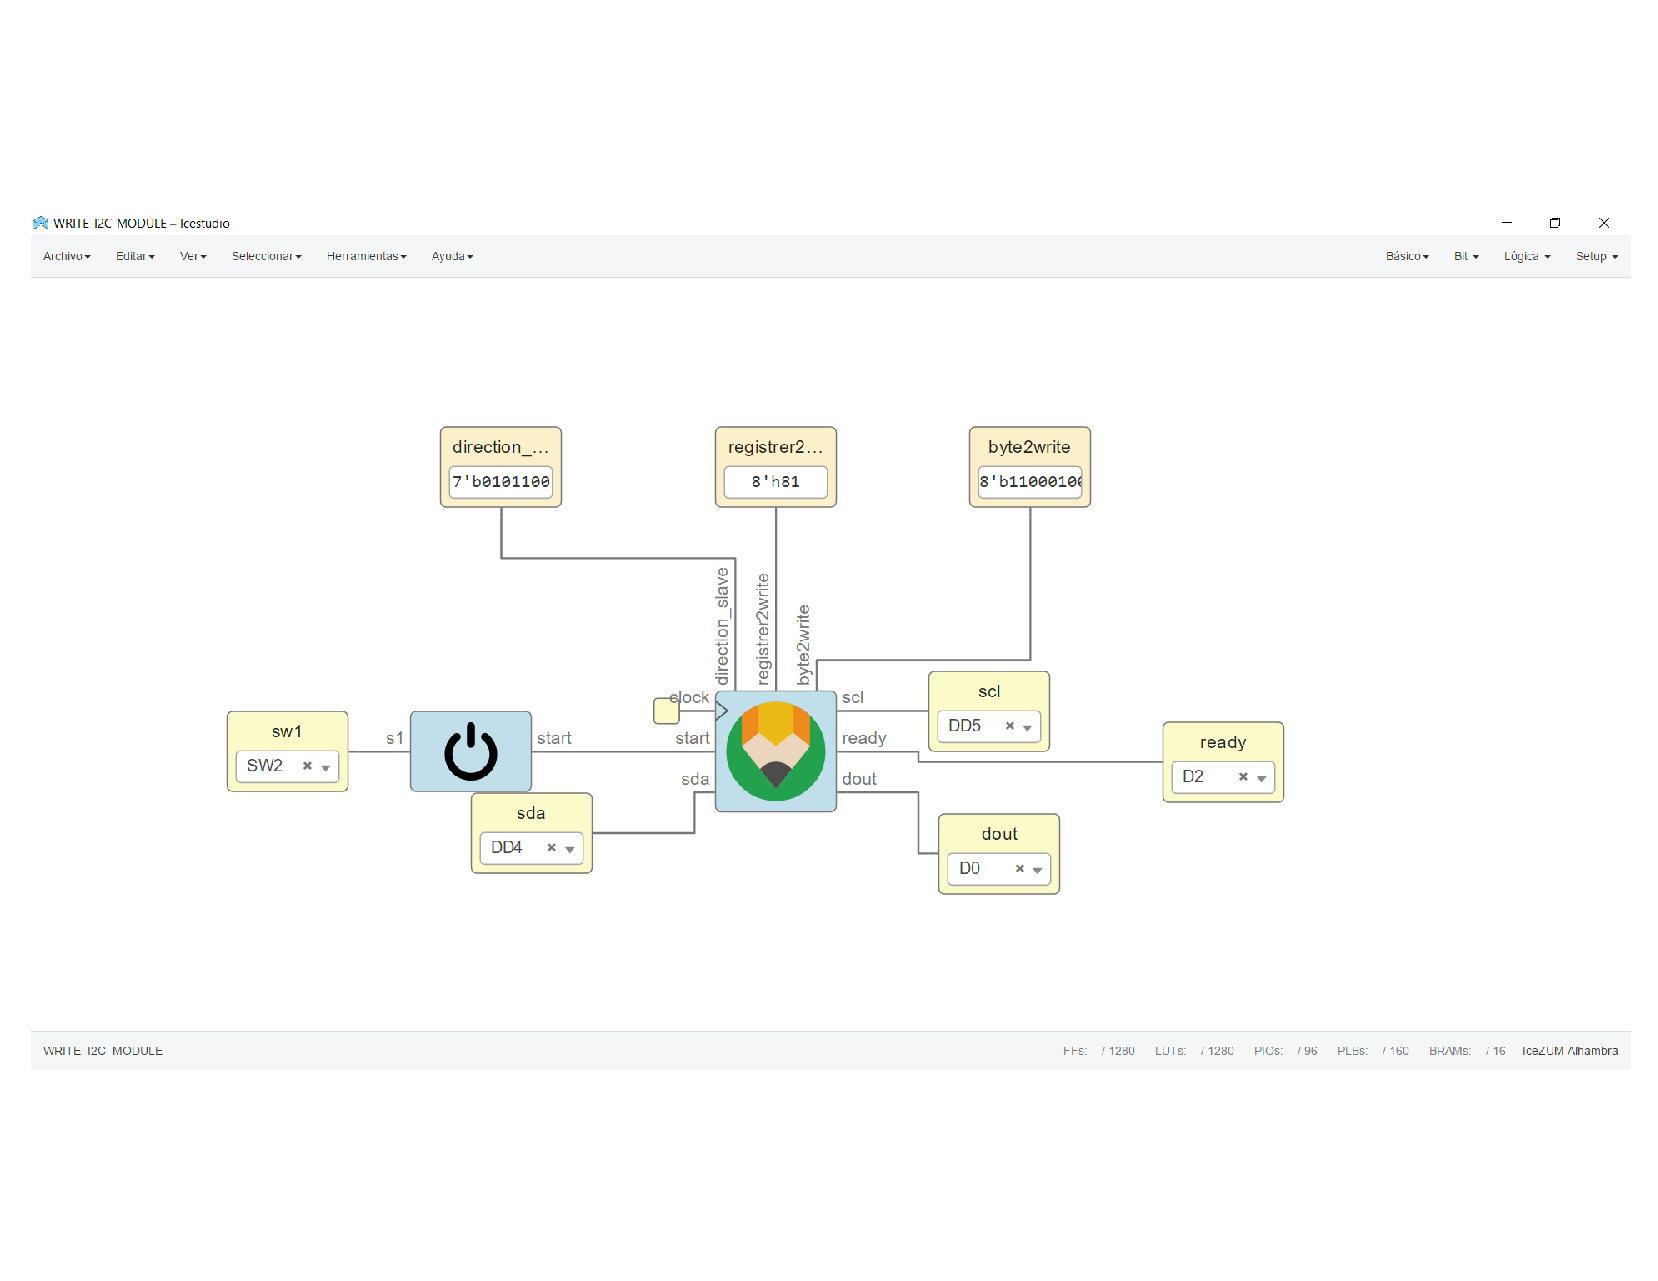
\includegraphics[trim = 0mm 0mm 0mm 0mm, clip,scale=0.4]{imagenes/EstadoArte/Write_i2c_module.pdf}
	\caption{Escritura I2C IceStudio alto nivel.}
	\label{fig:Write_i2c_module}
\end{figure}

Así, si una persona no experimentada con este tipo de código y cuyo fin no es entenderlo quiere hacer uso de eso no deberá de bajar mucho de nivel.\newline
No obstante, existe la posibilidad de que se requieran cambiar valores como la frecuencia de reloj, el modo de operación i2c...etc.
Para ello podemos bajar de nivel e introducirnos en el módulo en cuestión, en este caso, haciendo doble clic, como aparece en la figura \ref{fig:Write_i2c_module2}: 

\begin{figure}[H]
	\center
	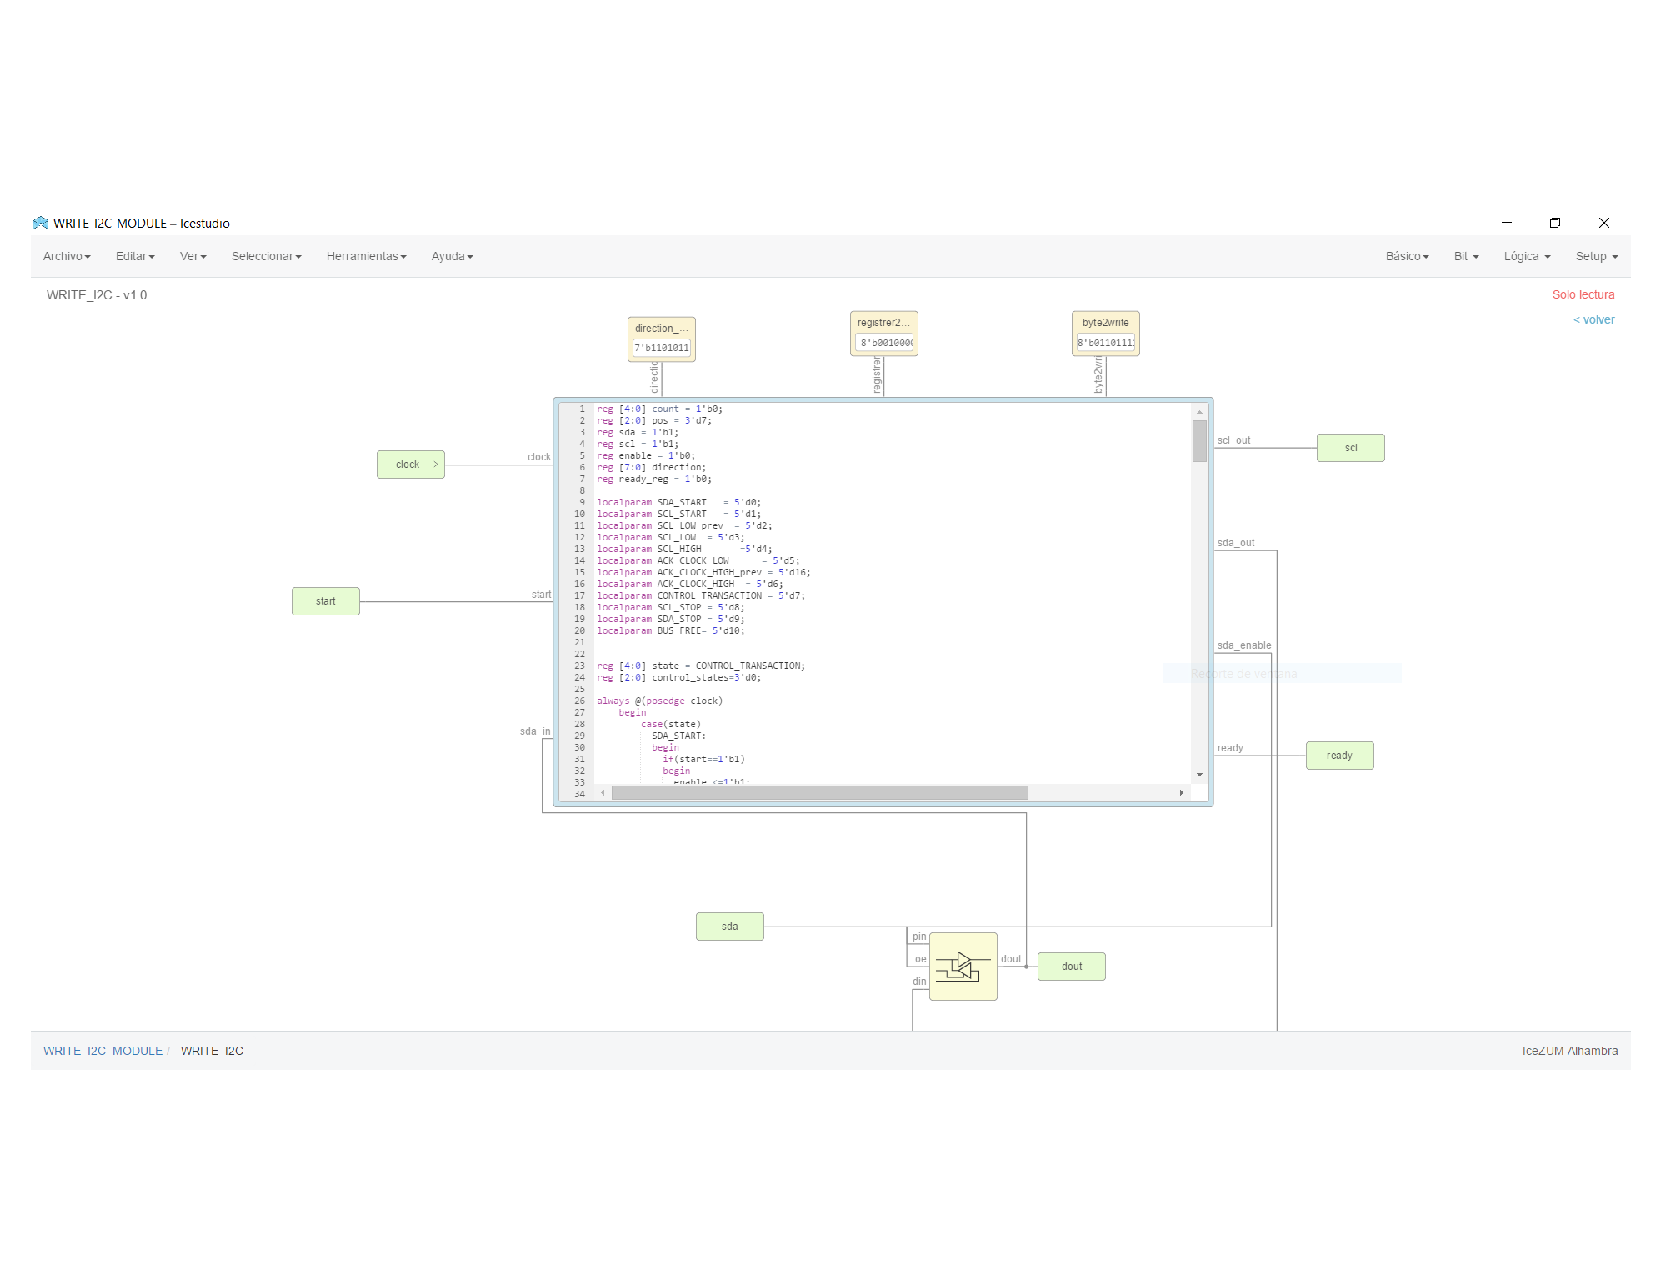
\includegraphics[trim = 0mm 0mm 0mm 0mm, clip,scale=0.4]{imagenes/EstadoArte/Write_i2c_module2.pdf}
	\caption{Escritura I2C IceStudio bajo nivel.}
	\label{fig:Write_i2c_module2}
\end{figure}

Se podría decir entonces que se ha bajado un nivel más de abstracción, pudiendo entrar ahora en detalles hardware más específicos si fuese necesario. \newline

En la antetior demostración se ha podido ver una de las ventajas de IceStudio. La modularidad permite configurar el nivel de abstracción.
Para ello hace falta una biblioteca de módulos, algunos de los cuáles serán desarrollados a lo largo de este trabajo, otros de ellos, están siendo trabajados, y pueden encontrarse en el siguiente enlace: 

\href{https://groups.google.com/forum/#!topic/fpga-wars-explorando-el-lado-libre/I3ZnqKlfh5M}{Foro de Google con discusión sobre temas y módulos para IceStudio.}


%%%%%%%%%%%%%%%%%%%%%%%%%%%%%%%%%%%%%%%%%%%%%%%%%
\section{Cohexistencia Microcontrolador-FPGA}
\subsection{Diferencia microcontrolador-FPGA}
En un principio puede parecer que un procesador y FPGA son dispositivos similares porque ambos pueden realizar ciertas tareas pre-configuradas. Lo cierto es que al prozundizar se pueden encontrar mas diferencias que similitudes. Ambos son capaces de implementar una función de transferencia, pero la forma en la que lo hacen es diferente para cada uno de ellos.\newline

Así, podríamos ver las FPGA y los microcontroladores como una caja negra en la que tenemos unas entradas y ciertas salidas.\newline


\begin{figure}[H]
	\center
	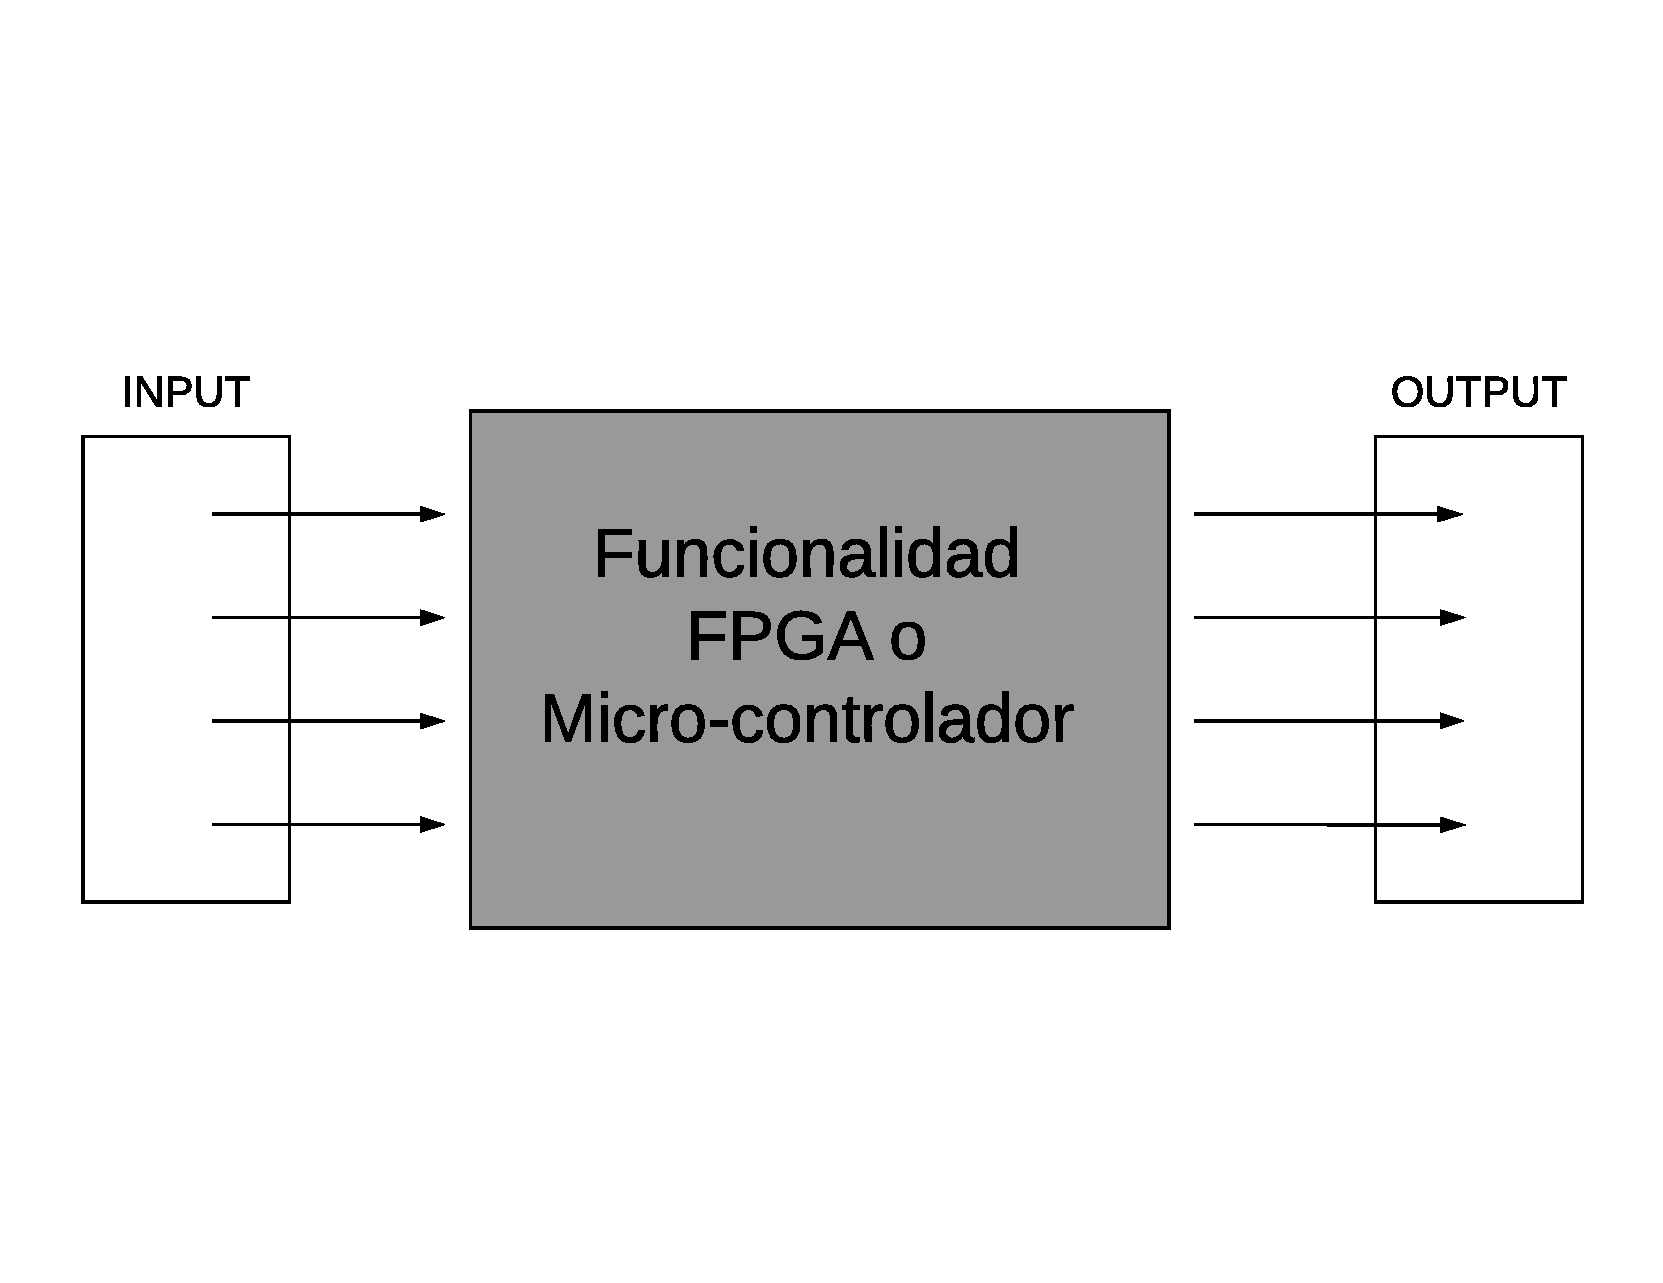
\includegraphics[trim = 0mm 30mm 0mm 30mm, clip,scale=0.4]{imagenes/EstadoArte/funcionalidad_FPGA_micro.pdf}
	\caption{Funcionalidad FPGA y Micro-controlador.}
	\label{fig:funcionalidad_FPGA_micro}
\end{figure}

Para comprobar de forma resumida como implementan de manera diferente esa función de transferencia, se explicará de forma muy resumida la forma de trabajar con un procesador. \newline
Un procesador contiene una serie de instrucciones que realizan operaciones sobre operaciones binarias (sumar, incrementar, leer y escribir de la memoria). Dependiendo del tipo de procesador y de su arquitectura tenemos más o menos instrucciones asociadas, siendo este aspecto uno de los mas importante que determinan su rendimiento.

\textbf{Arquitectura procesador}

Se dispone de una serie de registros, una memoria para almacenar la información y una pila de instrucciones, que contiene el programa que va a ejecutarse en código máquina, además de un relój.\newline

Su modo de funcionamiento a alto nivel; en cada ciclo de reloj el procesador lee de su pila de instrucciones los valores necesarios, llama a la instrucción oportuna y ejecuta un determinando cálculo.

Como se argumentó en el capítulo , al implementar un diseño lógico en una FPGA, se está modificando una matriz de conexiones físicas. Modificando esa matriz de conexiones se pueden implementar diferentes bloques de funcionalidad, es decir, se podría ver como varias funciones de transferencia en un mismo sistema. En la imágen \ref{fig:puertas_logicas} se puede ver una representación de un ejemplo real de como están implementadas las conexiones físicas de puertas lógicas en una FPGA, y de como eso permite tener módulos independientes unos de otros. Además, notese el problema de la memoria en una FPGA, siendo esta el número total de puertas lógicas físicas que pueden ser utilizadas;
\begin{center}
\begin{figure}[H]
	\center
	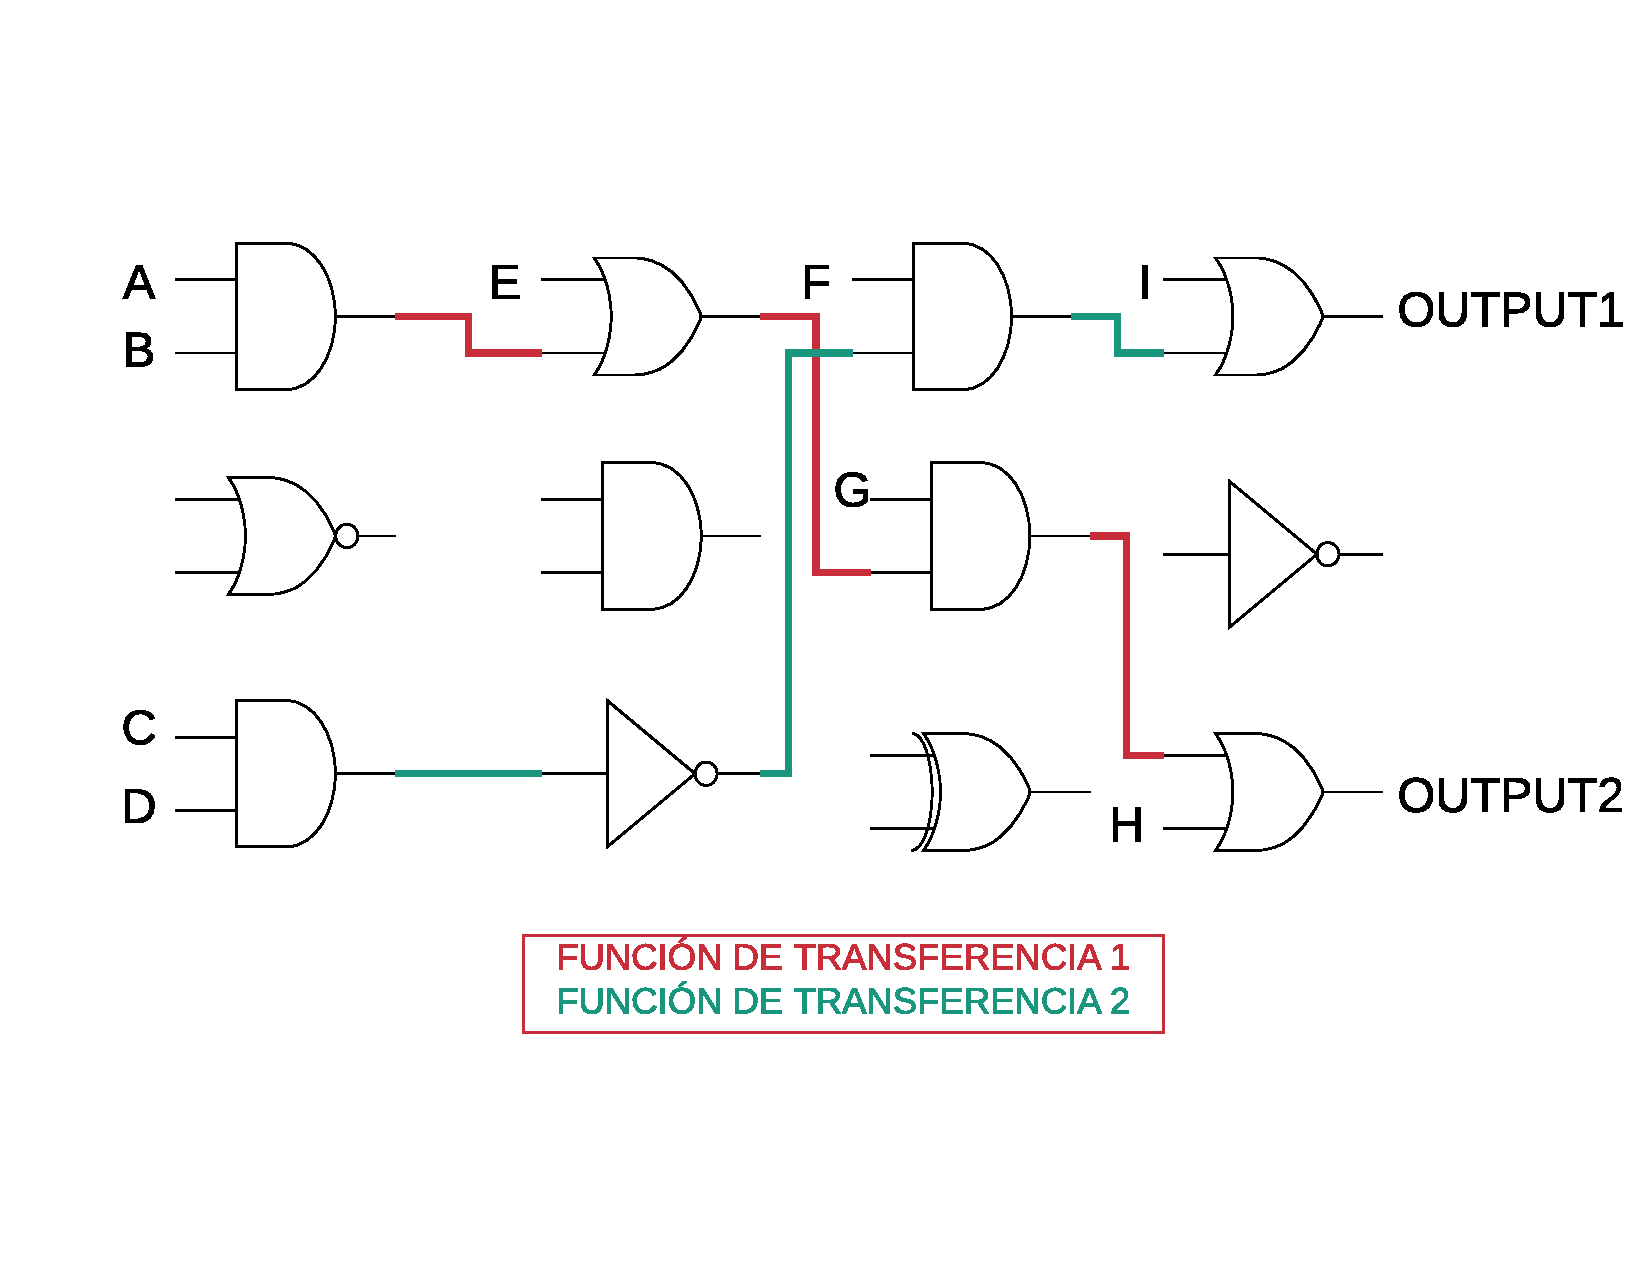
\includegraphics[scale=0.4]{imagenes/EstadoArte/puertas_logicas.pdf}
	\caption{Puertas lógicas despues de una implementación hardware.}
	\label{fig:puertas_logicas}
\end{figure}
\end{center} 

\subsection{Necesidad}

Se imagina un ejemplo real el que se quieren monitorizar con exactitud 4 diferentes sensores provenientes del exterior, de una manera exacta y a la velocidad del reloj, siendo necesario además una posterior actuación por parte del sistema. El diagrama de bloques del flujo de trabajo en un procesador que implemente lo anterior podría parecerse al siguiente:

\tikzstyle{block_circle} = [draw, fill=blue!20, circle, 
minimum height=3em, minimum width=6em]
\tikzstyle{block_rectangle} = [draw, fill=blue!20, rectangle, 
minimum height=3em, minimum width=6em]
%\tikzstyle{sum} = [draw, fill=blue!20, circle, node distance=1cm]
\tikzstyle{input} = [coordinate]
\tikzstyle{output} = [coordinate]
%\tikzstyle{pinstyle} = [pin edge={to-,thin,black}]

% The block diagram code is probably more verbose than necessary
\begin{center}
\begin{tikzpicture}[auto, node distance=2cm,>=latex']
	% We start by placing the blocks
	\node [input, name=input] {};
	\node [block_circle, right of=input] (Sensor1) {Sensor1};
	\node [block_rectangle, right of= Sensor1, node distance=3cm] (actuador1) {actuador1};
	\node [block_circle, right of=actuador1,node distance=3cm] (Sensor2) {Sensor2};
	\node [block_rectangle, right of= Sensor2, node distance=3cm] (actuador2) {actuador2};
	\node [block_circle, below of=actuador2,node distance=3cm] (Sensor3) {Sensor3};
	\node [block_rectangle, left of= Sensor3, node distance=3cm] (actuador3) {actuador3};
	\node [block_circle, left of=actuador3,node distance=3cm] (Sensor4) {Sensor4};
	\node [block_rectangle, left of= Sensor4, node distance=3cm] (actuador4) {actuador4};
	
	
	% We draw an edge between the controller and system block to 
	% calculate the coordinate u. We need it to place the measurement block. 
	
	% Once the nodes are placed, connecting them is easy. 
	\draw [draw,->] (Sensor1) -- node {} (actuador1);
	\draw [draw,->] (actuador1) -- node {} (Sensor2);
	\draw [draw,->] (Sensor2) -- node {} (actuador2);
	\draw [draw,->] (actuador2) -- node {} (Sensor3);
	\draw [draw,->] (Sensor3) -- node {} (actuador3);
	\draw [draw,->] (actuador3) -- node {} (Sensor4);
	\draw [draw,->] (Sensor4) -- node {} (actuador4);   
	
	
	
	
\end{tikzpicture}
\end{center}

Así, el usuario final de este sistema, deberá de manera cíclica comprobar cada sensor y su posterior actuación, dejando de cumplir entonces las especificaciones de tiempo. \newline
Si se trabajase con interrupciones se configurarían las diferentes interrupciones externas o se podrían usar ejecutivos cíclicos para acercarse a esos requerimientos finales. No obstante, cualquiera de estas soluciones, no dejan de ser una aproximación.\newline

En cambio, con el uso de un FPGA, el diagrama de bloques del flujo de trabajo tendría el siguiente aspecto:

\tikzstyle{block} = [draw, fill=blue!20, rectangle, 
minimum height=3em, minimum width=6em]
%\tikzstyle{sum} = [draw, fill=blue!20, circle, node distance=1cm]
\tikzstyle{input} = [coordinate]
\tikzstyle{output} = [coordinate]
%\tikzstyle{pinstyle} = [pin edge={to-,thin,black}]
\begin{center}

% The block diagram code is probably more verbose than necessary
\begin{tikzpicture}[auto, node distance=4cm,>=latex']
% We start by placing the blocks
\node [block] (sensor1) {Sensor1};
\node [block, right of=input] (function1) {$F_{1}$};
\node [block, right of= function1, node distance=4cm] (actuar) {actuadores};


% We draw an edge between the controller and system block to 
% calculate the coordinate u. We need it to place the measurement block. 

% Once the nodes are placed, connecting them is easy. 
\draw [draw,->] (sensor1) -- node {$$} (function1);
\draw [draw,->] (function1) -- node {$$} (actuar);



\end{tikzpicture}
\end{center}

\begin{center}
\begin{tikzpicture}[auto, node distance=4cm,>=latex']
% We start by placing the blocks
\node [block] (sensor2) {Sensor2};
\node [block, right of=input] (function2) {$F_{2}$};
\node [block, right of= function2, node distance=4cm] (actuar) {actuadores};


% We draw an edge between the controller and system block to 
% calculate the coordinate u. We need it to place the measurement block. 

% Once the nodes are placed, connecting them is easy. 
\draw [draw,->] (sensor2) -- node {$$} (function2);
\draw [draw,->] (function2) -- node {$$} (actuar);



\end{tikzpicture}
\end{center}

\begin{center}
\begin{tikzpicture}[auto, node distance=4cm,>=latex']
% We start by placing the blocks
\node [block] (sensor3) {Sensor3};
\node [block, right of=input] (function3) {$F_{3}$};
\node [block, right of= function3, node distance=4cm] (actuar) {actuadores};


% We draw an edge between the controller and system block to 
% calculate the coordinate u. We need it to place the measurement block. 

% Once the nodes are placed, connecting them is easy. 
\draw [draw,->] (sensor3) -- node {$$} (function3);
\draw [draw,->] (function3) -- node {$$} (actuar);



\end{tikzpicture}
\end{center}

\begin{center}
\begin{tikzpicture}[auto, node distance=4cm,>=latex']
% We start by placing the blocks
\node [block] (sensor4) {Sensor4};
\node [block, right of=input] (function4) {$F_{4}$};
\node [block, right of= function1, node distance=4cm] (actuar) {actuadores};


% We draw an edge between the controller and system block to 
% calculate the coordinate u. We need it to place the measurement block. 

% Once the nodes are placed, connecting them is easy. 
\draw [draw,->] (sensor4) -- node {$$} (function4);
\draw [draw,->] (function4) -- node {$$} (actuar);



\end{tikzpicture}
\end{center}



Se implementarían diferentes funciones de transferencia para cada uno de los bloques a desarrollar, pudiendo ejecutarse estos en paralelo. \newline

No obstante, no siempre es necesario un ejecutivo en paralelo, y no solo puede no ser necesario sino que podría ser perjudicial. Cuando un sistema debe ser secuencial, ¿porqué utilizar una implementación de naturaleza paralela?. \newline

Es muy común tener sistemas donde conviene poder implementar ambos tipos de funcionamiento, por eso una coexistencia FPGA- Micro-controlador podría ser suficiente para adaptarse a los requerimientos. \newline

En la imagen \ref{fig:bipedo} se puede ver como ejemplo real de un sistema bípedo, el cuál se explicará con mas detalle en los siguientes capítulos:

\begin{center}
	\begin{figure}[H]
		\center
		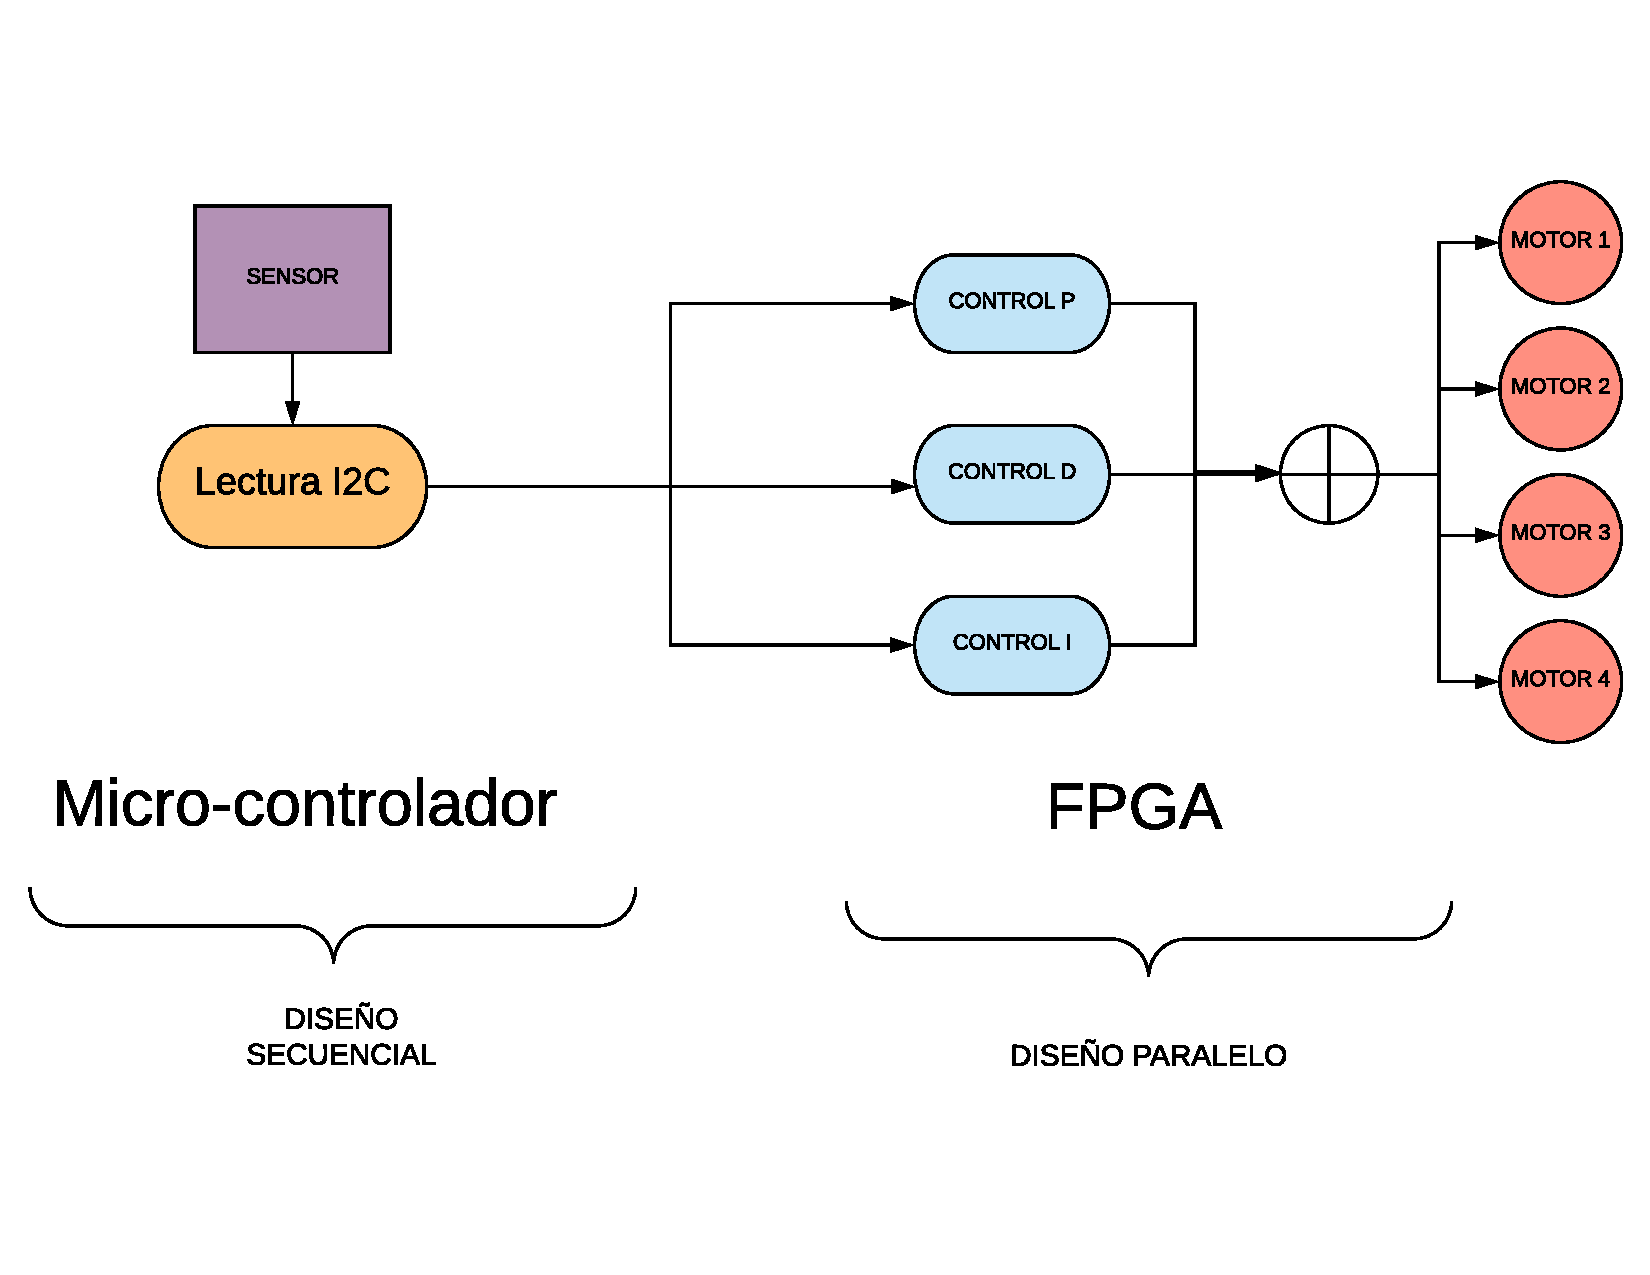
\includegraphics[scale=0.5]{imagenes/EstadoArte/bipedo.pdf}
		\caption{Sistema bipedo coexistencia Micro-FPGA.}
		\label{fig:bipedo}
	\end{figure}
\end{center}
%%%%%%%%%%%%%%%%%%%%%%%%%%%%%%%%%%%%%%%%%%%%%%%%%
\section{Robótica educativa, motivaciones y necesidad.}

La robótica se puede considerar sin duda como una de las areas tecnológicas con mas auge de la actualidad y basada en el estudio de los robots. que son sistemas compuestos por mecanismos que le permiten hacer movimientos y realizar tareas especificas, programables e inteligentes. \newline

Dependiendo de la aplicación por tanto, la robótica puede extenderse y generar beneficios no solo en la industria sino también en las aulas de clase, posibilitando la aparición de nuevos sistemas de aprendizaje.\newline

Además en un mundo cuyo futuro va encaminado a la utilización de robots para cualquier actividad, el acercamiento desde las aulas con estos sistemas posibilita su desarrollo tecnológico a una edad temprana, siendo más fácil su integración a una edad adulta.\newline

Algunos beneficios de la robótica educativa son expuestos a continuación:  
\begin{itemize}
	\item Impulsa la iniciativa y la creatividad
	\item Mayor sociabilización
	\item Incentiva el pensamiento algoritimico y matematico
	\item Trabajo en equipo
	\item Resolución de problemas
	\item Aprendizaje activo
	\item Aumento de la autoestima
\end{itemize}

No obstante, para que la integración en las aulas de la robótica educativa sea aun mas fácil, los sistemas deben cumplir algunas características:

\begin{itemize}
	\item No es recomendable la integración a alto nivel tecnológico.
	\item Los robots deben ser de carácter amigable y divertido. 
	\item Los entornos de programación no deben ser complejos, y aunque su funcionalidad este algo limitada, tiene que llamar la atención del alumno y hacerle sentir cómodo.
	\item Es importante que el robot cuente con una serie de sensores y actuadores, unas entradas y salidas para que los resultados sean visuales.
\end{itemize}

Después de haber analizado cuáles son las ventajas de la electrónica digital, resulta conveniente poder acercar estos dos campos de conocimiento; electrónica digital-robótica educativa.\newline

Si la electrónica digital y el mundo de los robots están llamados a formar parte de nuestras vidas en un futuro cercano, la necesidad de un acercamiento a estos dos conceptos a edades tempranas es básico para un correcto avance de la tecnología. \newline

Con esta idea nace IceStudio, hacer amigable la electrónica digital para que los más pequeños puedan hacer uso de ella, y además, cumple todas las características antes expuestas.

\section{Sensores, actuadores y sistema de control }

$http://www.micronica.es/files/pdfs/SIHD/SIHD_Sens_Actu_EC.pdf$
$https://es.wikipedia.org/wiki/Sensor$

Antes de comenzar con el desarrollo del proyecto, es importante tener claro los conceptos de sensores, actuadores y elementos del sistema de control, los cuáles forman parte de cualquier plataforma robótica móvil. \newline

Cualquier instalación de control, ya sea robótica o inmotica, esta compuesta por tres componentes fundamentales:
\begin{itemize}
	\item Sensores
	\item Actuadores
	\item Sistema de control
\end{itemize}

Los sensores son dispositivos que recogen información del mundo que nos rodea y lo transforma en señales eléctricas que puedan ser asimiladas por un sistema de control. \newline

Así, el sistema de control recibe información del entorno sobre el que queremos realizar algún tipo de acción por medio de los sensores, es la función de transferencia del sistema, a partir de unas entradas de tipo conocido, son generadas unas salidas, normalmente, dependientes de las entradas.

Estas salidas son denominadas actuadores, que son dispositivos que, siguiendo los parametros dados por el sistema de control realizan acciones que repercuten en el entorno. \newline

\textsl{Ejemplo: Un sensor indica al sistema de control la intensidad lumínica de nuestra habitación, el sistema de control reconoce que el nivel no es el adecuado para la lectura, y activa un actuador, en este caso, una luz, para contrarrestar ese nivel.}

A la hora de elegir un determinado sensor, es importante conocer su modo de operación, para poder configurar o mantener sistemas que los incorporen. Existen diferentes tipos de sensores según:

\begin{itemize}
	\item Tipo de salida: \begin{itemize}
		\item Analogicos
		\item Binarios
		\item Digitales
	\end{itemize} 
	
	\item Estructura interna: \begin{itemize}
		\item Pasivos
		\item Activos
	\end{itemize}
	
	\item Tipo de parámetros capaces de detectar
\end{itemize}
 A continuación se muestran algunos de los más interesantes para el desarrollo del proyecto:

\begin{table}[H]
	\begin{center}
	\begin{tabular}{|c|l|l|}
		\hline
		\textbf{Magnitud}                                                                       & \multicolumn{1}{c|}{\textbf{Transductor}} & \multicolumn{1}{c|}{\textbf{Característica}} \\ \hline
		\multirow{}{}{\begin{tabular}[c]{@{}c@{}}Posición lineal y\\   angular\end{tabular}}  & Potenciómetro                             & Analógica                                    \\ \cline{2-3} 
		& Encoder                                   & Digital                                      \\ \cline{2-3} 
		& Sensor Hall                               & Digital                                      \\ \hline
		\multirow{}{}{\begin{tabular}[c]{@{}c@{}}Velocidad\\   lineal y angular\end{tabular}} & Dinamo tacométrica                        & Analógica                                    \\ \cline{2-3} 
		& Encoder                                   & Digital                                      \\ \cline{2-3} 
		& Detector inductivo                        & Digital                                      \\ \cline{2-3} 
		& Servo-inclinómetros                       & A/D                                          \\ \cline{2-3} 
		& RVDT                                      & Analógica                                    \\ \cline{2-3} 
		& Giróscopo                                 & Digital                                      \\ \hline
		\multirow{}{}{Aceleración}                                                            & Acelerómetro                              & Analógico                                    \\ \cline{2-3} 
		& Servo-accelerómetros                      &                                              \\ \hline
		\multirow{}{}{Visión artificial}                                                      & Cámaras de video                          & Procesamiento digital                        \\ \cline{2-3} 
		& Cámaras CCD o CMOS                        & Procesamiento digital                        \\ \hline
	\end{tabular}
	\caption{Modo de operación de sensores.}
	\label{tabla:modo_operacion_sensores}
\end{center}
\end{table}

Otra clasificación posible es la del ámbito de aplicación, es decir, donde y para qué son usados estos sensores. 

De entre las carácterísticas técnicas más importantes de un sensor, y haciendo una introduccion al posible vocabulario que se utilizará, encontramos:

\begin{itemize}
	\item Rango de medida:  dominio en la magnitud medida en el que puede aplicarse el sensor.
	\item Precisión: es el error de medida máximo esperado.
	\item Offset o desviación de cero: valor de la variable de salida cuando la variable de entrada es nula.
	\item Sensibilidad de un sensor: suponiendo que es de entrada a salida y la variación de la magnitud de entrada.
	\item Resolución: mínima variación de la magnitud de entrada que puede detectarse a la salida.
	\item Derivas: son otras magnitudes, aparte de la medida como magnitud de entrada, que influyen en la variable de salida.
\end{itemize}

Por lo general, la señal de salida de estos sensores no es apta para su lectura directa y a veces tampoco para su procesado, por lo que se usan circuitos de acondicionamiento. 

\textbf{imagenes de sensores}

Los actuadores son los dispositivos que permiten al sistema de control ‘actuar’ sobre el ‘mundo real’ para realizar las acciones deseadas. Uno de los actuadores mas conocidos son los motores, el cuál será muy utilizado a lo largo de esta aplicación. 




%
\chapter{Self-Balancing Robot}\label{sec: BalancingRobot}
In this chapter, the objective is to address the inverted pendulum problem through the usage of an FPGA in coexistence with a microcontroller. For this, in the respective chapters, physics of a self-balancing robot, the calculation of its structure, the sensors and actuators used, the control system and the design and manufacture of a PCB that solves in a more adequate way some problems of those previously raised, will be treated.A communication between FPGA/Microcontroller will be used and a more global version of the proposed system will be given, with a general block diagram. \newline

It starts with a problem description (section \ref{sec:Descripcion_balancin}) to continue with a brief high level solution (section \ref{sec:Diseno}). To finish, an explanation of each blocks will be described (section \ref{sec:Implementacion}).

\section{Problem Description} \label{sec:Descripcion_balancin}

To understand the work to be done, the problem of inverted pendulum will be briefly enunciated, whose solution has given rise to many very famous tools nowadays, one of them, called \textit{SegWay} (Figure \ref{fig:segway}).

\begin{figure}[H]
	\center
	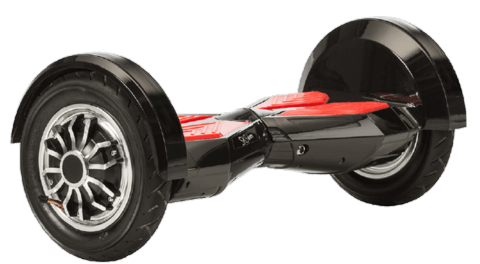
\includegraphics[trim = 0mm 0mm 0mm 0mm, clip,scale=0.4]{imagenes/Balancing_robot/segway}
	\caption{Commercial Segway.}
	\label{fig:segway}
\end{figure}


\begin{definicion}Pendulum \cite{Pendulum}: It is a physical system that can oscillate under the gravitational action or other physical characteristic (elasticity, for example) and that is configured by a mass suspended from a point or a horizontal axis by a wire, a rod, or other device that is used to measure time. \newline
\end{definicion}
As can be imagined, an inverted pendulum has the aspect shown in Figure \ref{fig:pendulo}. 

\begin{figure}[H]
	\center
	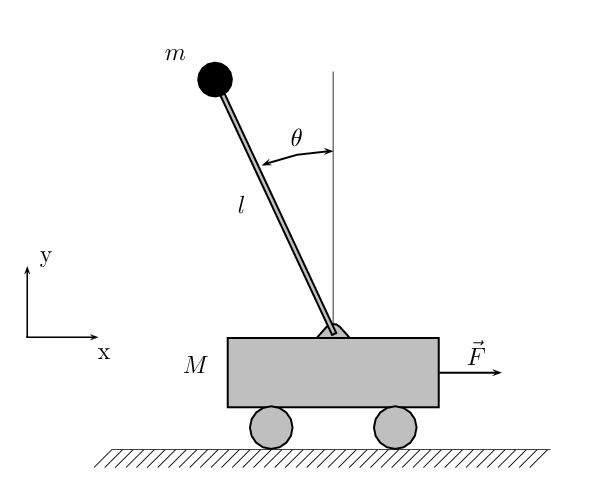
\includegraphics[trim = 0mm 0mm 0mm 0mm, clip,scale=1.6]{imagenes/Balancing_robot/pendulo}
	\caption{Inverted pendulum representation.}
	\label{fig:pendulo}
\end{figure}

Consists of a pendulum where the mass center is located above the point or balancing axis. As expected, this layout gives the system static instability. We recall that a system is stable when its gravity center is closer to the support horizontal plane. \newline

The base of this project will therefore be to correct this instability and is part of one of the most famous problems in terms of control theory and systems dynamics. 

\newpage
\section{System Design}\label{sec:Diseno}

By i2c communication with an IMU sensor, the microcontroller obtains the current angle of the system. Obtained the angle by the microcontroller a communication of serial type sends it to the FPGA in a binary format of 1 byte for the integral part and 1 byte for the decimal part. A shield with a driver of DC motors connected to the FPGA brings the possibility of varying the speed and direction of two DC motors that allow the stabilization of the system. The speed of the motors for a correct correction of the angle is calculated by a basic PD controller implemented in the FPGA.

\begin{center}
	\begin{figure}[H]
		\center
		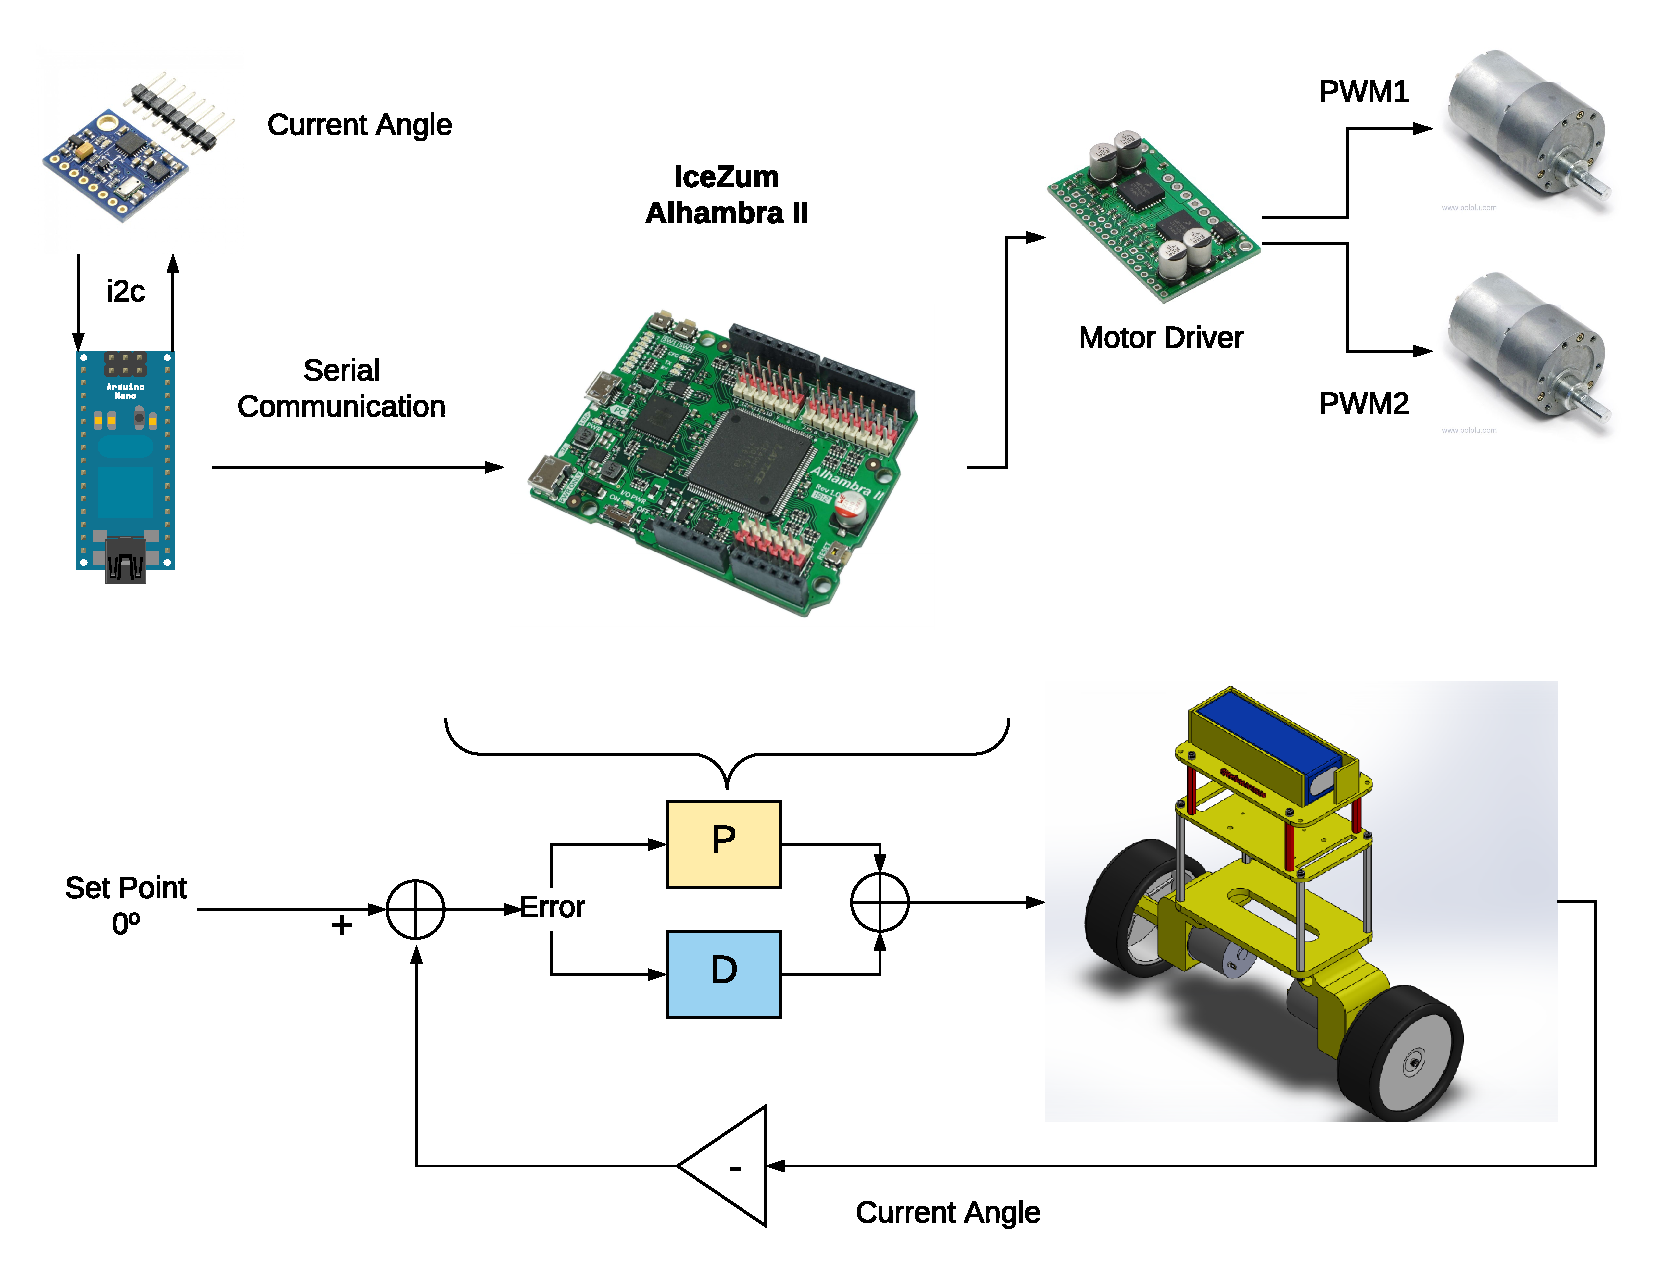
\includegraphics[trim = 0mm 0mm 0mm 0mm,clip, angle=0, scale = 0.4]{imagenes/Balancing_Robot/final.pdf}
		\caption{Final block diagram.}
		\label{fig:final}
	\end{figure}
\end{center}

%En esta sección se propone una solución al problema planteado proporcionando esta con un alto nivel de abstracción. En la sección \ref{sec:Implementacion} se profundizará aún más en los detalles de los diferentes sub-sistemas que aquí se exponen.

The following chapters will go deeper into each of the previous blocks that form the final solution (Figure \ref{fig:final}). 


\newpage
\section{System Implementation}\label{sec:Implementacion}
\subsection{Mechanical Structure Manufacturing}
Knowing the physics of a self-balancing robot \cite{6845943} \cite{7112017} and with the aim, therefore, of solving the classic problem of the inverted pendulum, the mechanical structure of the Figures \ref{fig:EnsanBalanceFront}, \ref{fig:EnsanBalanceLateral} y \ref{fig:EnsanBalanceCab},designed with SolidWorks is proposed and from which the rest of the components will be assembled.

\begin{center}
	\begin{figure}[H]
		\center
		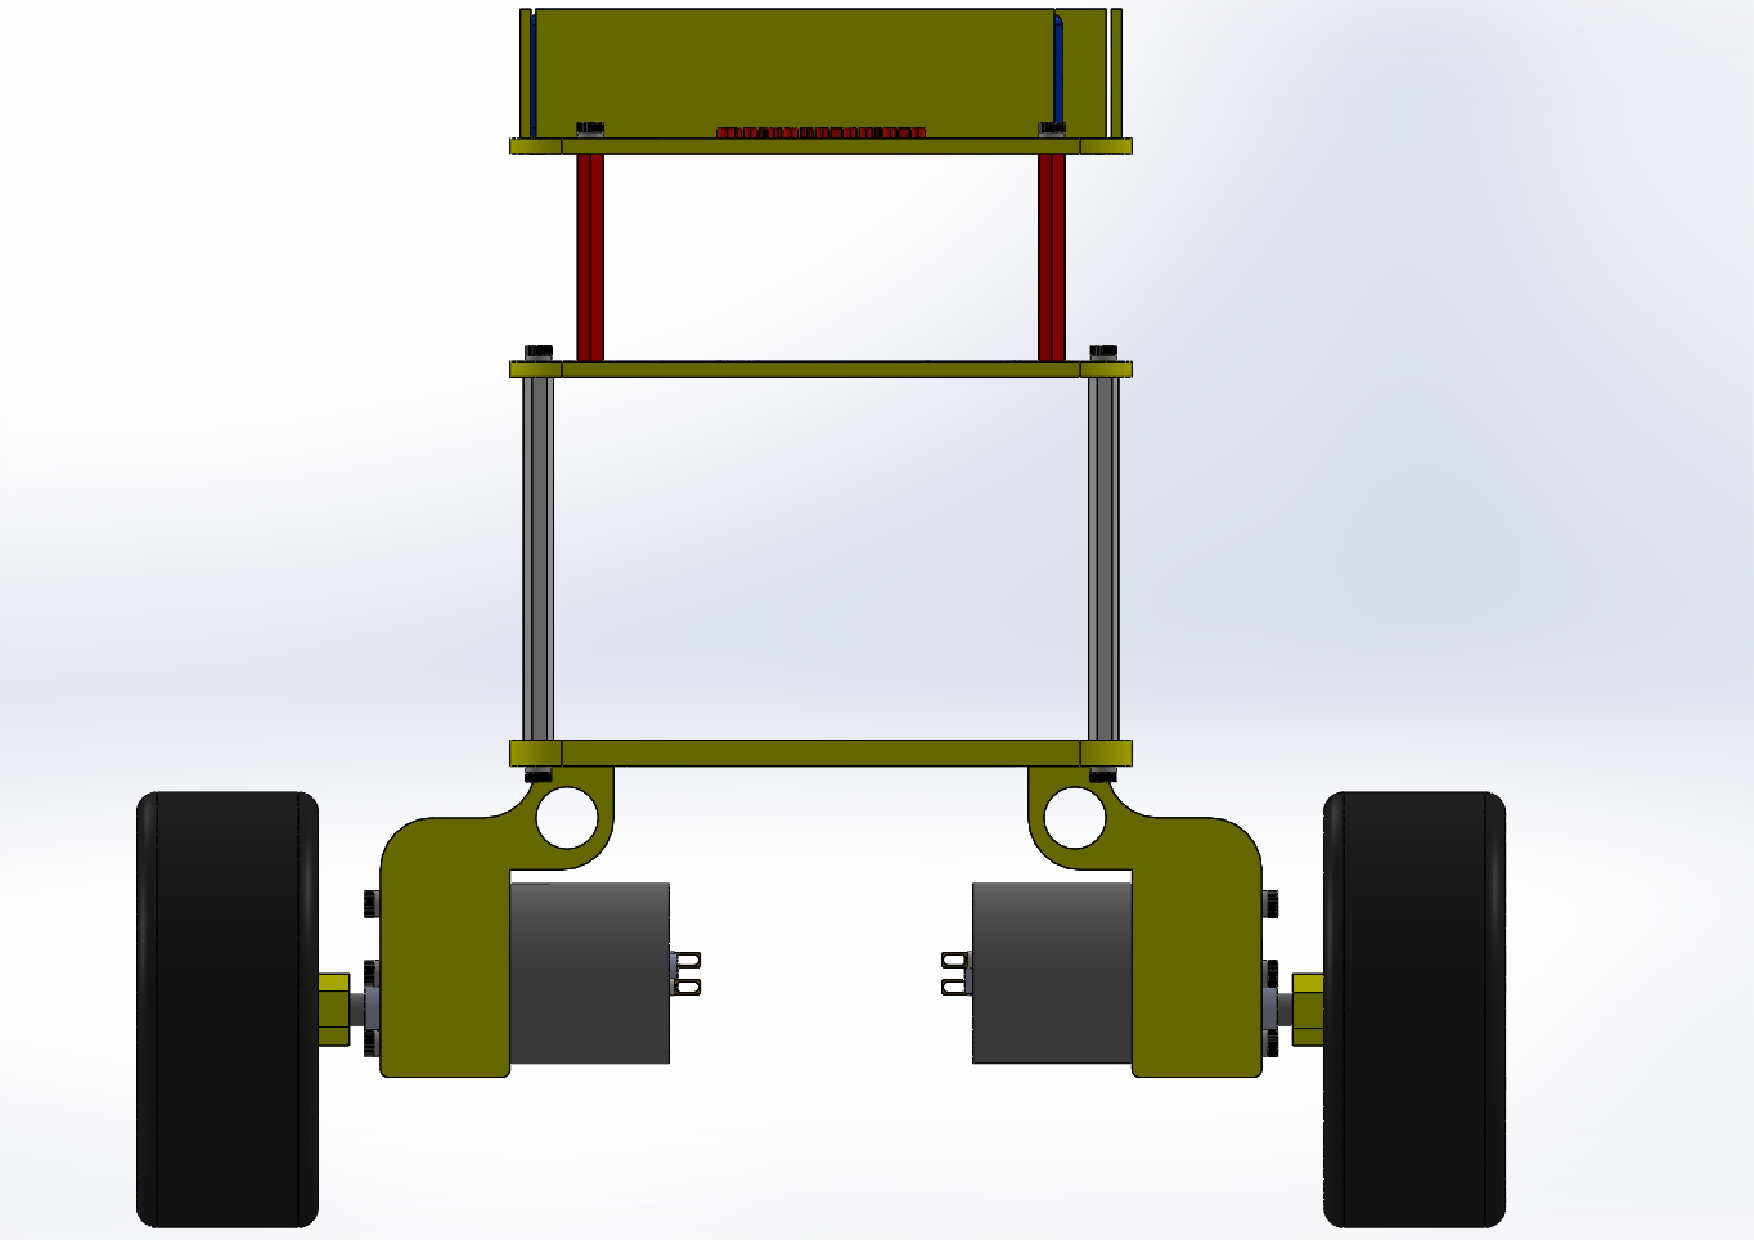
\includegraphics[trim = 1cm 0mm 2.7cm 0mm,clip, angle=0, scale = 0.4]{imagenes/Balancing_Robot/EnsanBalanceFront.PDF}
		\caption{Frontal view Balancing Robot.}
		\label{fig:EnsanBalanceFront}
	\end{figure}
\end{center}

\begin{center}
	\begin{figure}[H]
		\center
		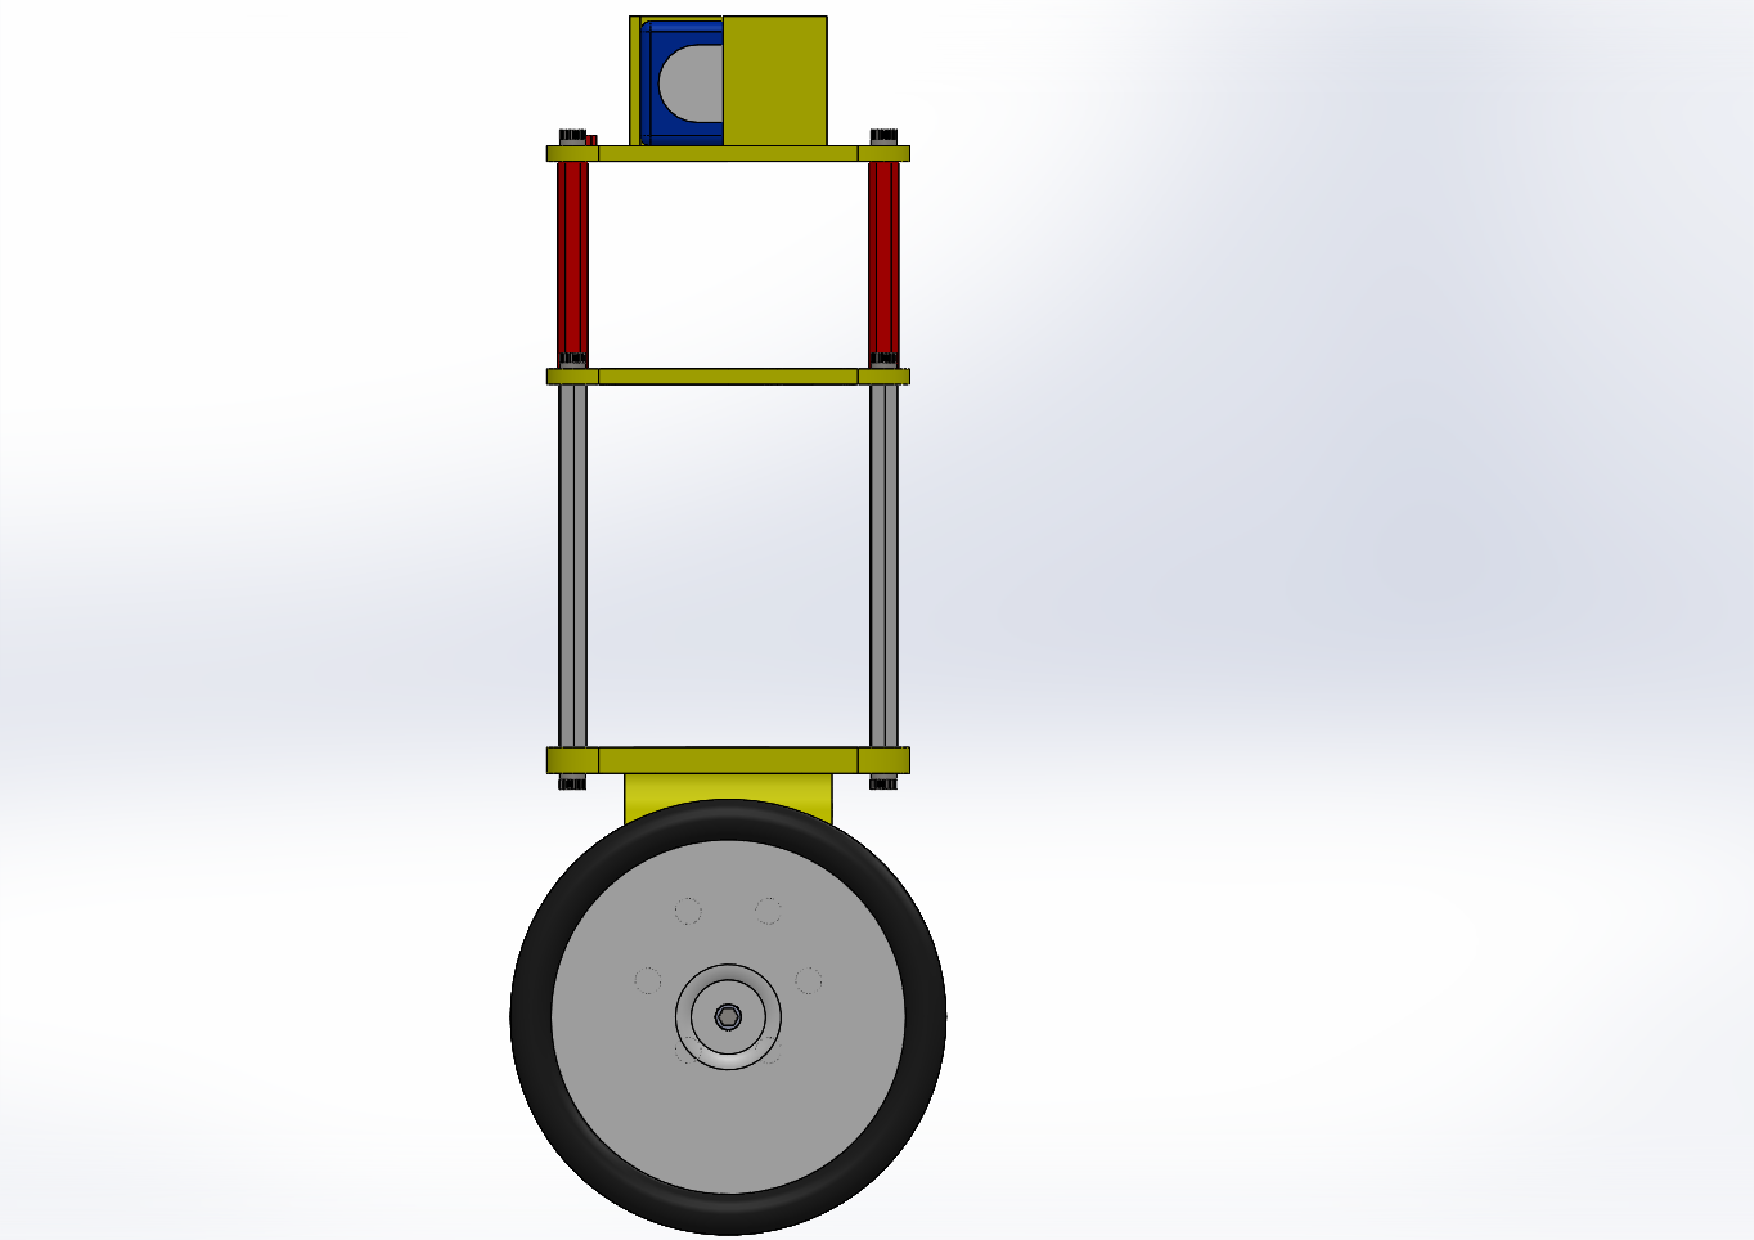
\includegraphics[trim = 5cm 0mm 10cm 0mm,clip, angle=0, scale = 0.5]{imagenes/Balancing_Robot/EnsanBalanceLateral.PDF}
		\caption{Lateral view derecha Balancing Robot.}
		\label{fig:EnsanBalanceLateral}
	\end{figure}
\end{center}

\begin{center}
	\begin{figure}[H]
		\center
		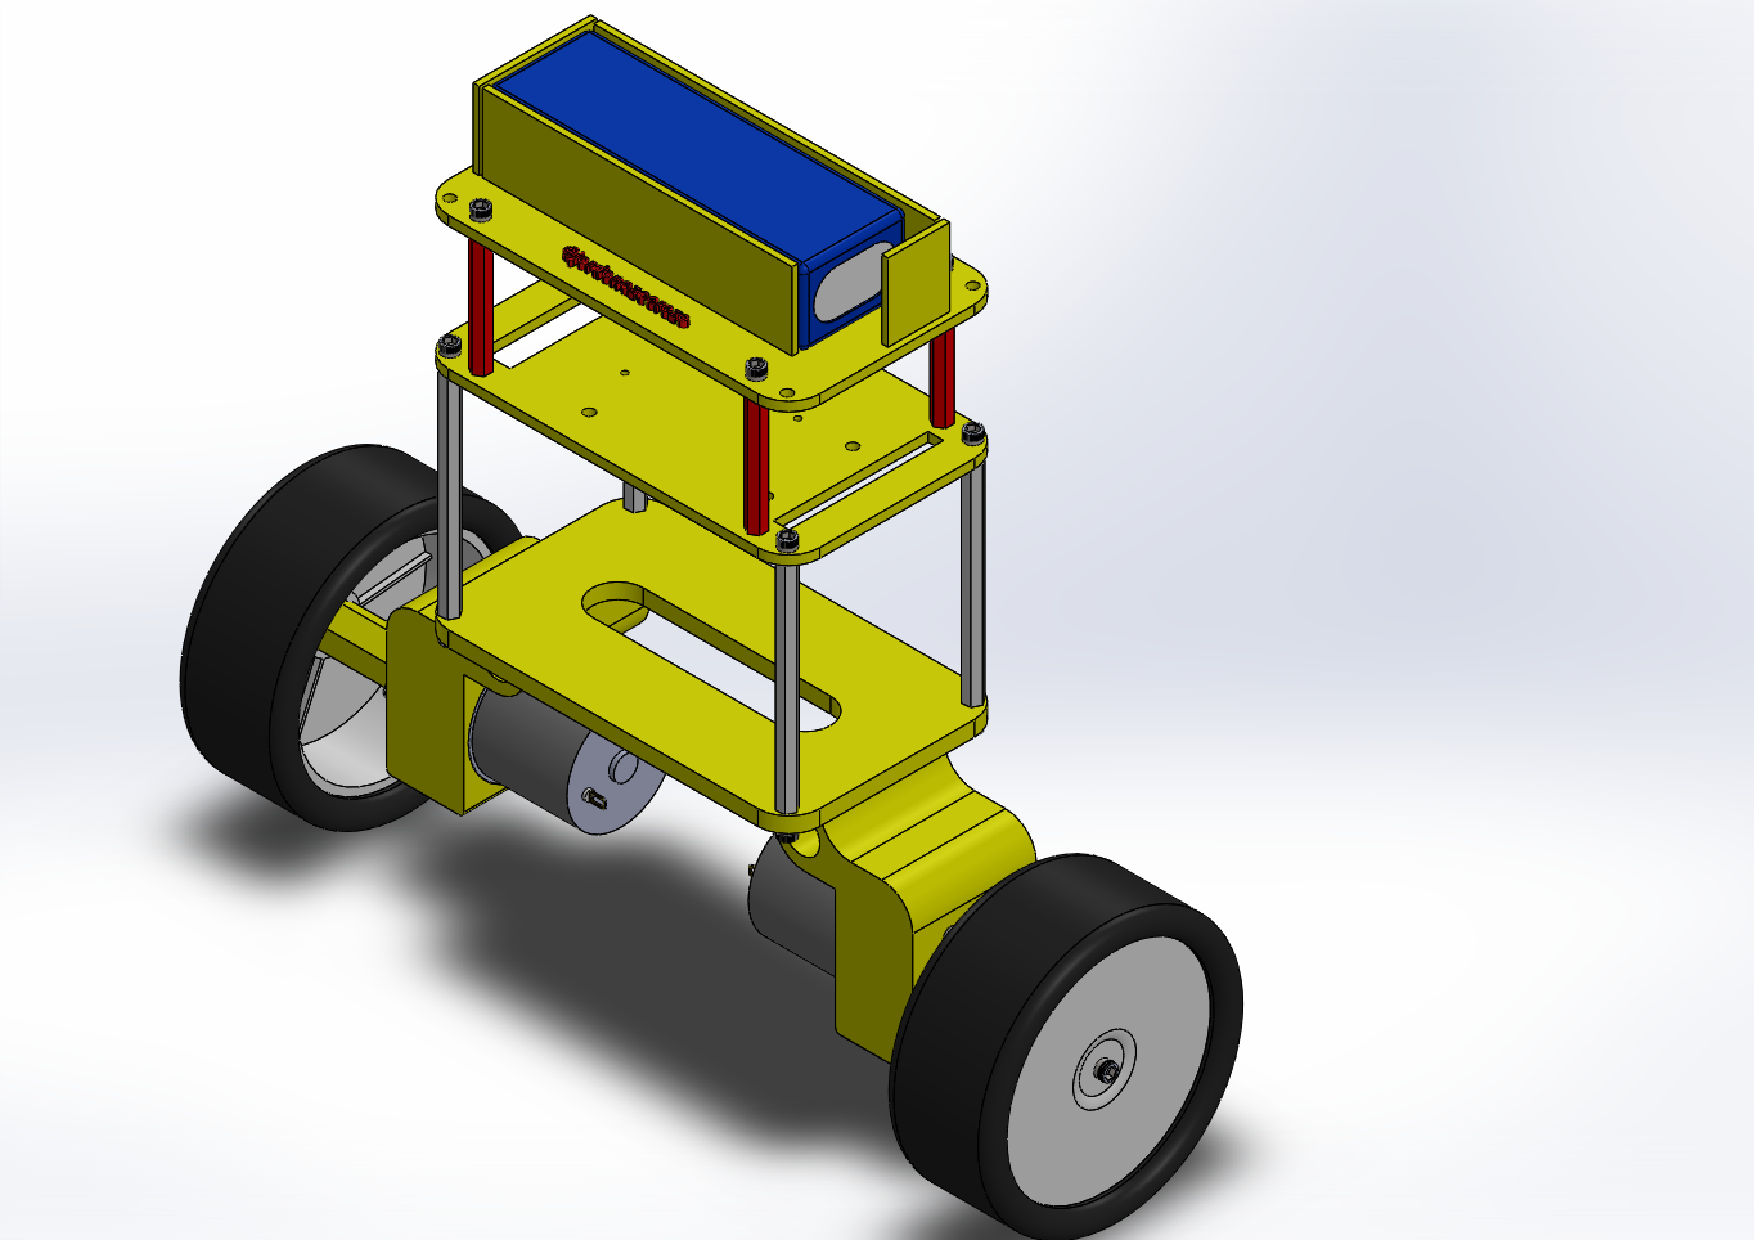
\includegraphics[trim = 20mm 0mm 8cm 0mm,clip, angle=0, scale = 0.5]{imagenes/Balancing_Robot/EnsanBalanceCab.PDF}
		\caption{Balancing Robot perspective.}
		\label{fig:EnsanBalanceCab}
	\end{figure}
\end{center}

Different aspects of the design of this structure are considered, which are directly related to the physics of a self-balance Robot, and with it, of the inverted pendulum. \newline
As argued in section \ref{sec:Descripcion_balancin}, a system at rest is stable when its mass center is closer to the horizontal plane. If we consider that the nature of the proposed system is inherently unstable, it is necessary to know the best point where the mass center must be in order to allow a better stability. \newline

Assuming the of mathematical modeling characterization, it is therefore assumed that to achieve greater ease in stabilization, the center of mass should be placed above the midpoint of the vertical axis of our system. Therefore, we must consider the weight of all components for a placement that allows the above. \newline
In Figure \ref{fig:center_mass}, a SolidWorks calculation is represented from this mass center where there have only been considered the heavier components of the final system, which includes, DC motors, batteries, mechanical structures and wheels.

\begin{figure}[H]
	\center
	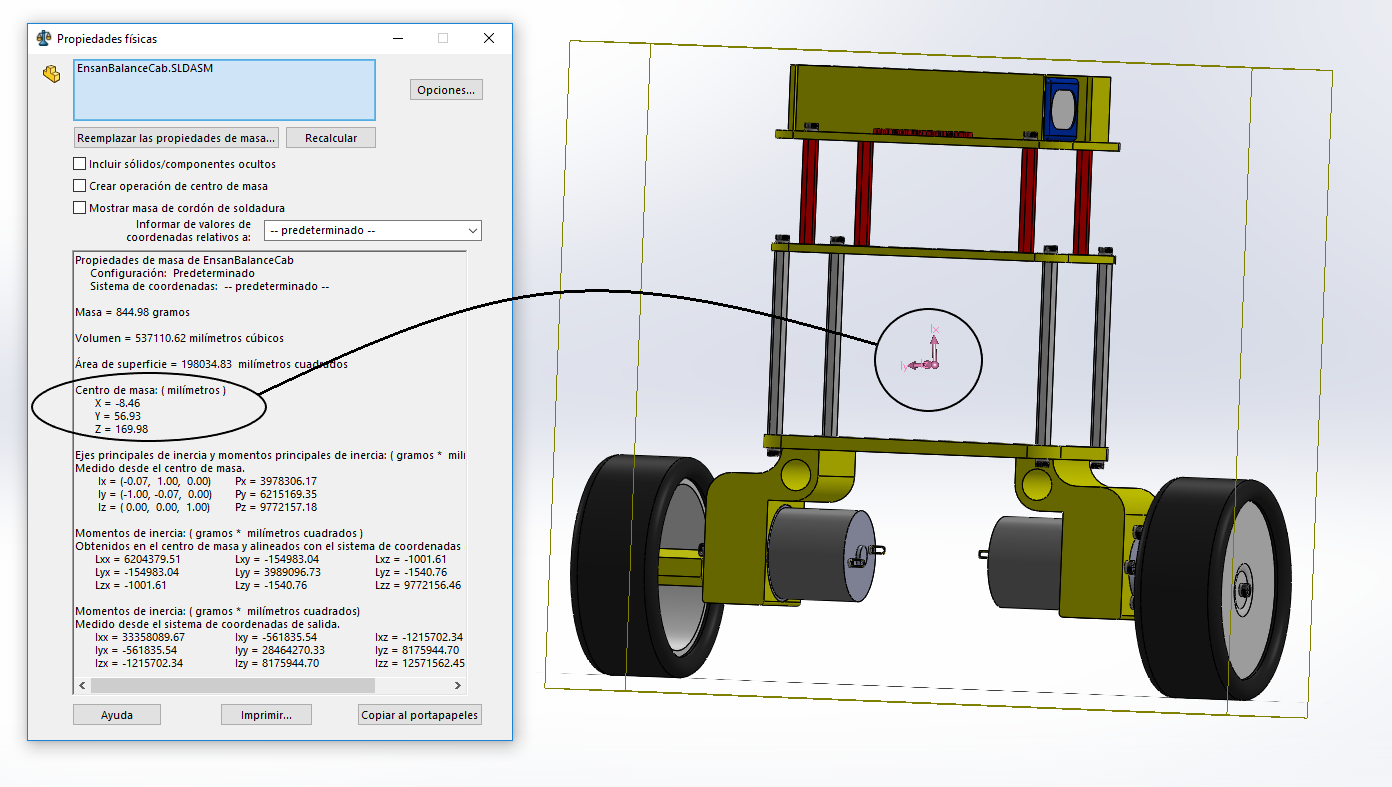
\includegraphics[scale=0.3]{imagenes/Balancing_robot/center_mass}
	\caption{Center of mass final system.}
	\label{fig:center_mass}
\end{figure}

\subsection{Inertial Measurement Unit MPU6050 in Arduino Nano}\label{sec:MPU6050}

A constant knowledge of the angle of the system is necessary for its analysis and correction, for this purpose the MPU6050 sensor has been used, connected by an i2c communication to an Arduino Nano. \newline

The MPU6050 is an Inertial Measure Unit (IMU) with 6 degrees of freedom (6DOF) manufactured by Invensense. It has an accelerometer and gyroscope and allows communication by both SPI and i2c bus. To correct some of the data collection problems, mentioned in section \ref{sec:IMU} it incorporates an internal processor (Digital Motion Processor, DMP) that executes data fusion algorithms (Motion Fusion) to combine the measurements of the internal sensors, avoiding having to perform the filters externally.\newline

Due to its low cost and big quality, this is one of the most used IMUs nowadays. In Figure \ref{fig:IMU1} a MPU6050 image is shown.

\begin{figure}[H]
	\center
	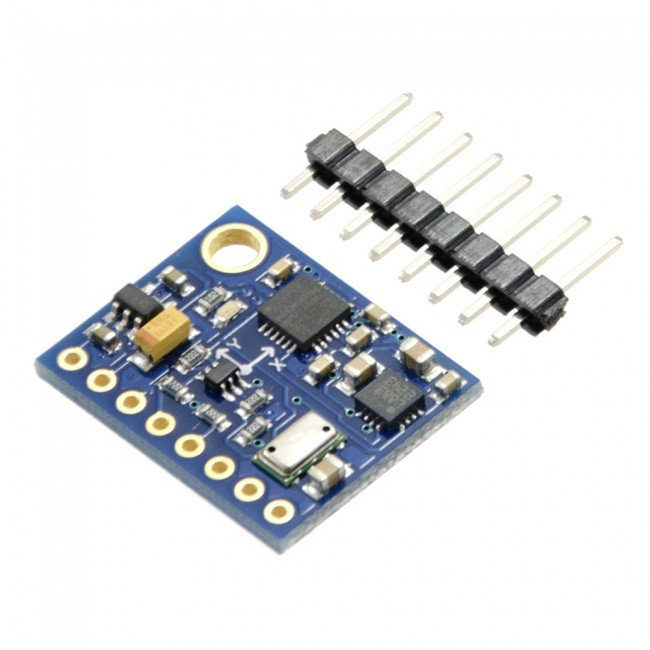
\includegraphics[scale=0.2]{imagenes/Balancing_robot/IMU1}
	\caption{MPU6050 IMU.}
	\label{fig:IMU1}
\end{figure}
\subsubsection{Pin-out}

Figure \ref{fig:MPU6050_schematic} shows the schematic connections diagram of the MPU6050.

\begin{figure}[H]
	\center
	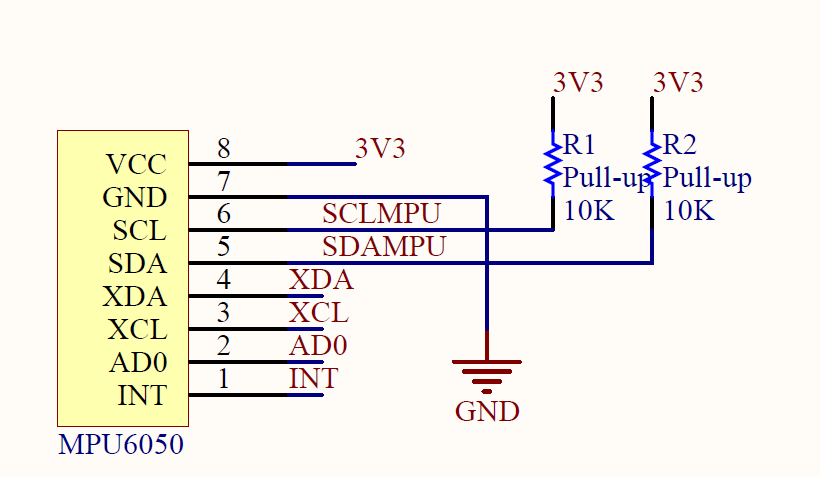
\includegraphics[scale=0.4]{imagenes/Balancing_robot/MPU6050_schematic}
	\caption{MPU6050 IMU.}
	\label{fig:MPU6050_schematic}
\end{figure}

It has a 3.3V power supply voltage. The clock pin for the I2C connection (Serial Clock Line, SCL) and the data pin (Serial Data Line, SDA) represent the connection for the bus with Arduino Nano. AD0 pin allows the user to change the address of the MPU (slave), which by default is 0x68h connected to GND. If it is connected to Vcc, the address changes to 0x69h. INT pin produces a signal on high when the data in issue is available from the MPU to be captured and will warn by an interruption to the Arduino Nano with the purpose to be obtained.\newline

\subsubsection{Arduino Nano Program}
For the Arduino Nano implementation it is used a library developed by Jeff Rowberg. The reason of the use of this library is because it incorporates the usage of the DMP. This use  exempts the microprocessor (Arduino Nano in this case) from a complex filtered and calculation with the purpose to obtain the values pitch, yaw and roll. A representation of this advantages are represented in Figure \ref{fig:DMPExample}.\newline
\begin{figure}[H]
	\center
	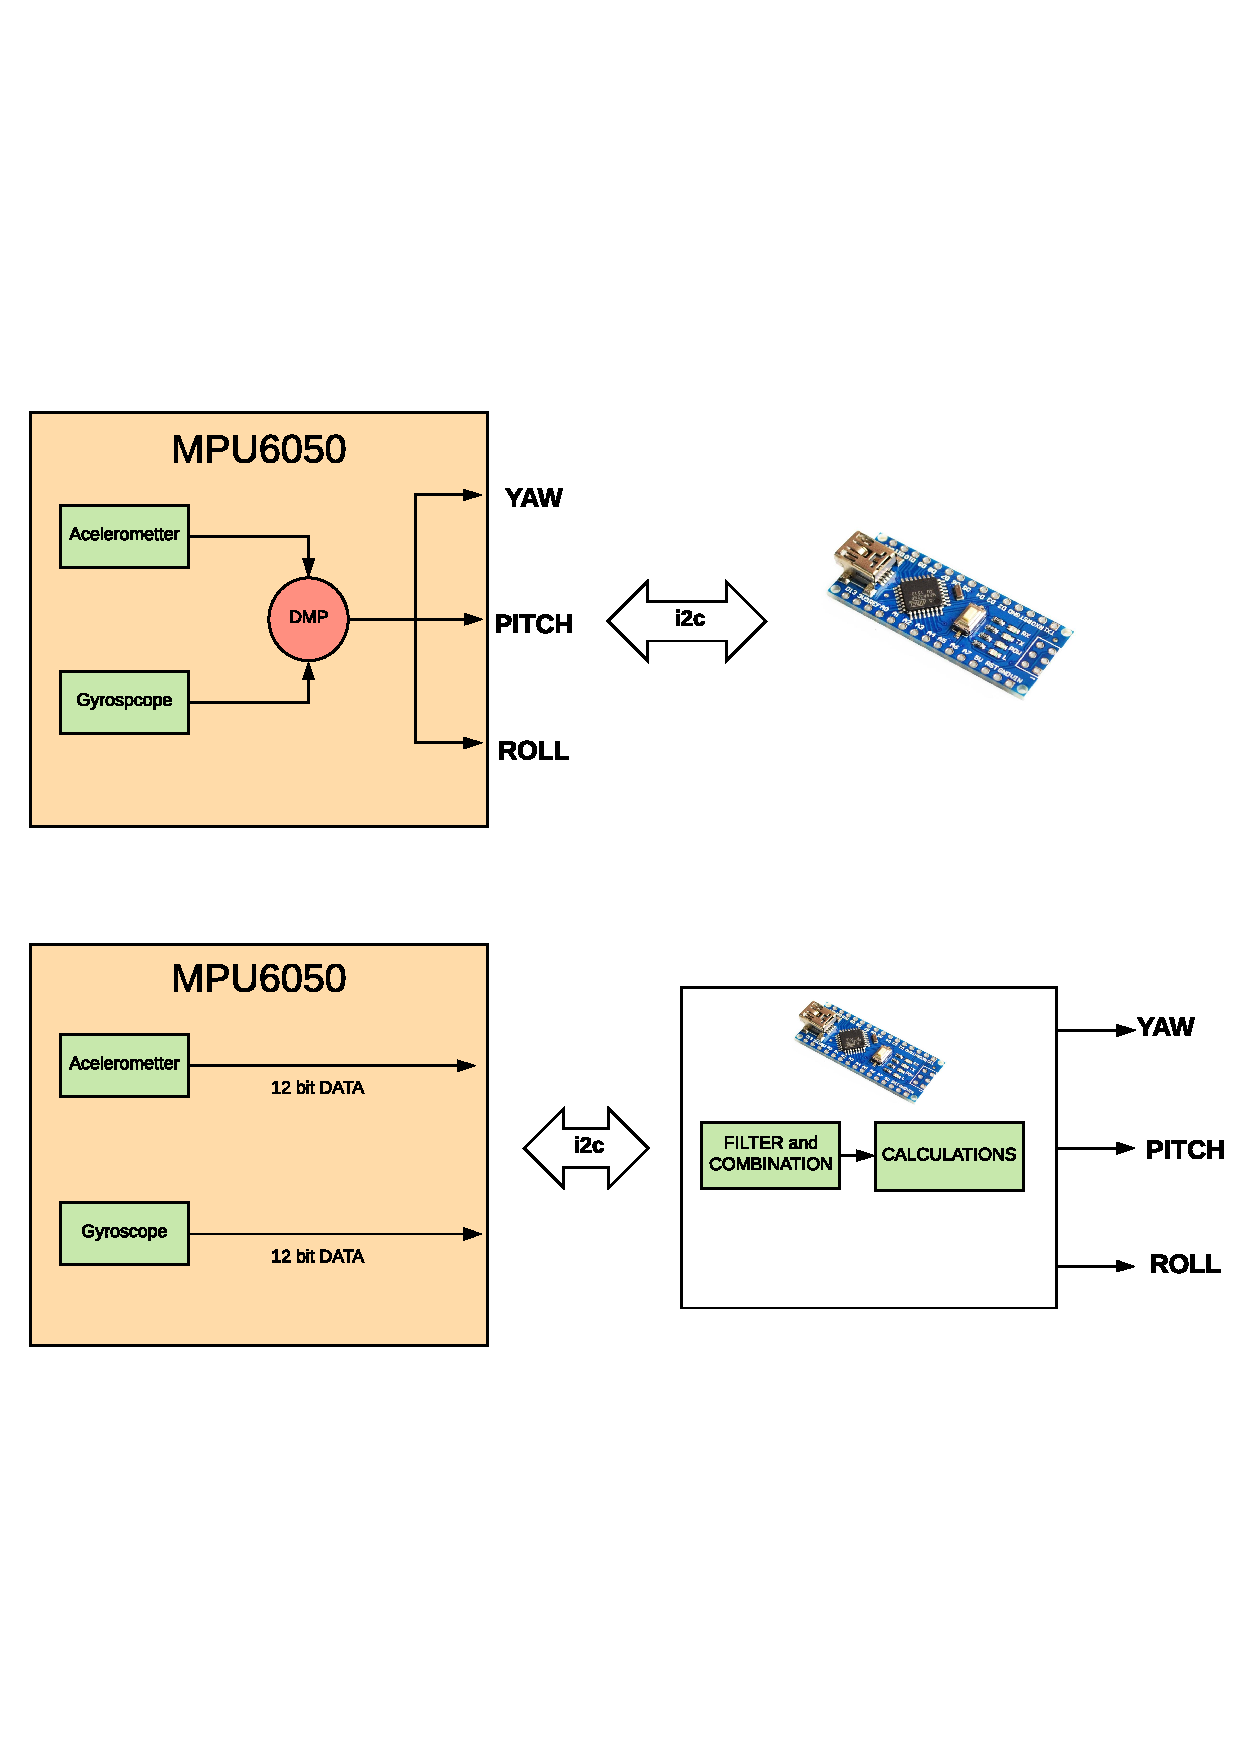
\includegraphics[trim = 0mm 4cm 0mm 2cm, clip,scale=0.6]{imagenes/Balancing_robot/DMPexample.pdf}
	\caption{Advantaje in the use of DMP.}
	\label{fig:DMPExample}
\end{figure} 


%An example of the obtained values by the sensor are shown in the figure.

%\textbf{foto de un ejemplo de los ángulos}

\subsection{PCB Implementation}\label{sec:PCB}

After featuring the entire system and considering the necessary connection diagram not only between the microcontroller and FPGA but also for the OV7670 (it uses in section \ref{sec: Cuadricoptero}) and the motor driver, it is convenient and appropriate a printed circuit that solves some noise problems, excessive cables, etc. \newline

The printed circuit contains the following components and behaviors:

\begin{itemize}
	\item A total of 28 pins on the outside of the PCB and arranged in the correct position for a fit in the IceZum Alhambra II board (Figure \ref{fig:pin_headers}), which allows to use as inputs or outputs the pins of the FPGA. In order to know the exact position of the pins on the plate, the Altium project was used, which is available on GitHub.
	
	\begin{figure}[H]
		\center
		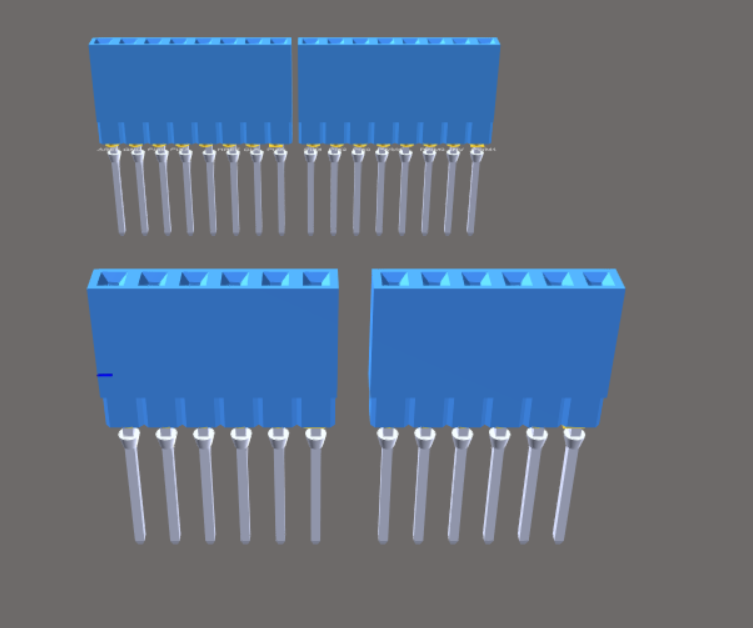
\includegraphics[scale=0.4]{imagenes/Balancing_robot/pin_headers.PNG}
		\caption{Pin headers for IceZum Alhambra II.}
		\label{fig:pin_headers}
	\end{figure}
	
	
	\item 4 VDC and 12 Volt GND connections to power the ESCs of the brushless motors of the aerial vehicle. For this, the component of figure \ref{fig:screw}, has been chosen, because it has adequate features of maximum temperature to which it may be subjected and which would be analyzed further on.
	
	\begin{figure}[H]
		\center
		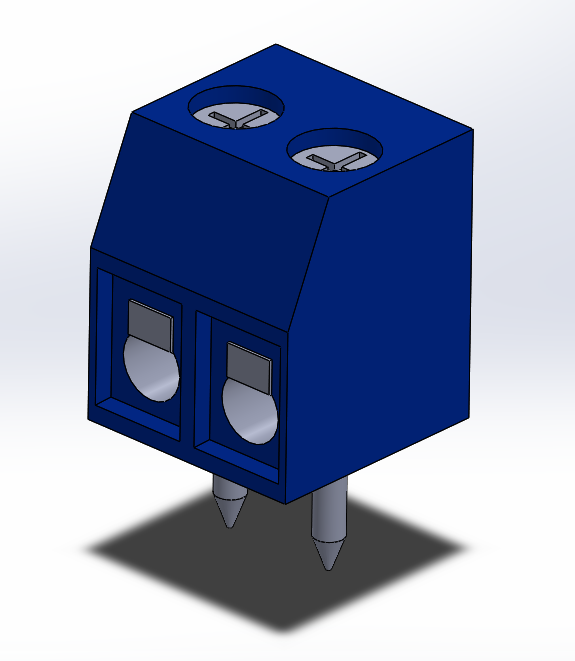
\includegraphics[scale=0.4]{imagenes/Balancing_robot/SCREW.PNG}
		\caption{Connector GND and VCC.}
		\label{fig:screw}
	\end{figure}
	
	
	\item A VCC and GND connection to feed the previous connections. This connector would go directly to a LIPO battery of 11.1V (3 cells) and 2200mAh. The fact of choosing this battery is due to the minimum voltage by which the ESCs of the brushless motors are fed, as well like the motors and the motor driver used for the self-balancing Robot. A more detailed analysis of the battery can be found in subsection \ref{sec:Bateria}
	
	\item Header pin modules for the MPU6050 connection previously described. (Figure \ref{fig:mpu6050_connector}).
		
		\begin{figure}[H]
			\center
			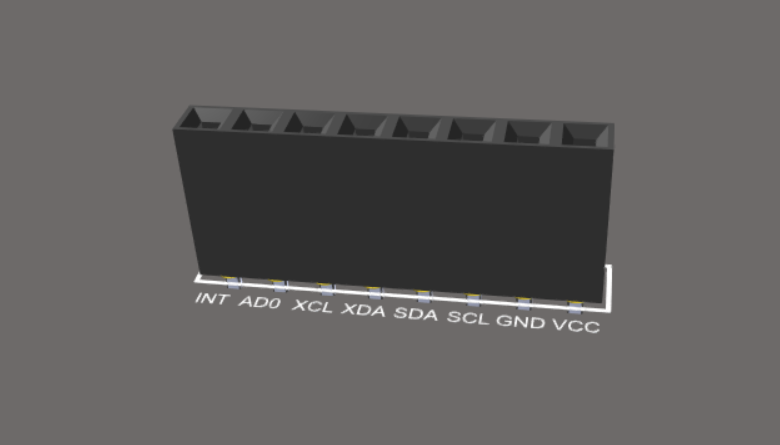
\includegraphics[scale=0.4]{imagenes/Balancing_robot/mpu6050_connector.PNG}
			\caption{Module MPU6050.}
			\label{fig:mpu6050_connector}
		\end{figure}
		
		\item An extension of the most important pins of the MPU6050 is made so that they can be used by the microcontroller in the case of angle analysis, as in this project, is part of a process governed by the microcontroller.
		
		\item Two jumpers connection (Figure \ref{fig:jumpers}) in I2C bus allow the user to decide who governs the SDA and SCL line, microcontroller or FPGA. 
		
		\begin{figure}[H]
			\center
			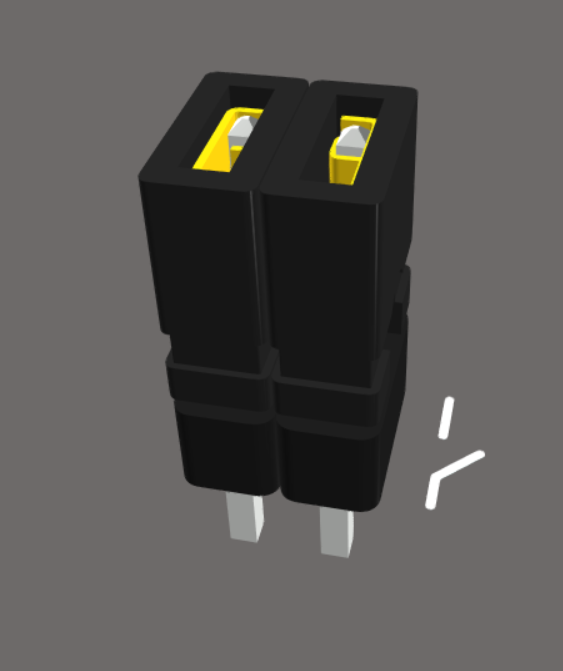
\includegraphics[scale=0.3]{imagenes/Balancing_robot/jumpers.PNG}
			\caption{Jumpers to configurate i2c MPU6050.}
			\label{fig:jumpers}
		\end{figure}	
	
		When hosting a bus line, it is not necessary to consider the thermal characteristics of the connector in issue, and when working at a relatively small frequency, the noise that the jumpers can introduce into the I2C communication may be accepted.
		\item A great part of actual microcontrollers works at 3.3-5V but the input voltage supported can go high to 12V, because of that it is taken advantage of the LIPO battery power and a new connector with two header pin is implemented that goes to VCC and GND which will power the microcontroller.	
		\item A module that can host the OV7670 camera (section \ref{sec: Cuadricoptero})formed by male headers pin and each of which will be attached to one of the FPGA's in-out pins, as will be seen later in the general schematic.
		\item A module that can host the driver of the DC motor used in this case and that allows direct connection with IceZum Alhambra II pins, for example, the pwm signal that will define the speed of the engines will be an output on one of the FPGA pins, and it should be an input to the motor driver.
		
		\item So that there are no errors in the I2C transmission, there’s a 4,7K$\Omega$ resistor in each of the lines.
	\end{itemize}	
	In Figures \ref{fig:top_3D}, \ref{fig:bottom_3D}, \ref{fig:Vista3D1}, \ref{fig:Vista3D2} is included a 3D representation of the final system with all its added component
	
	\begin{center}
		\begin{figure}[H]
			\center
			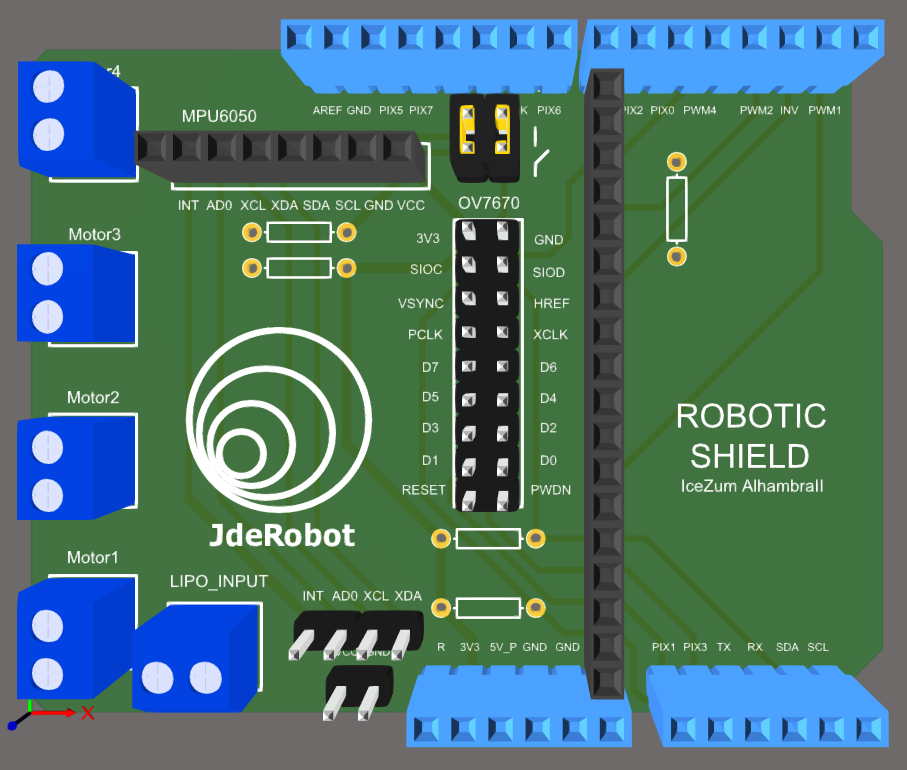
\includegraphics[scale=0.6]{imagenes/Balancing_Robot/top_3D.PNG}
			\caption{3D View of Shield for IceZum Alhambra II.}
			\label{fig:top_3D}
		\end{figure}
	\end{center}
	
	\begin{center}
		\begin{figure}[H]
			\center
			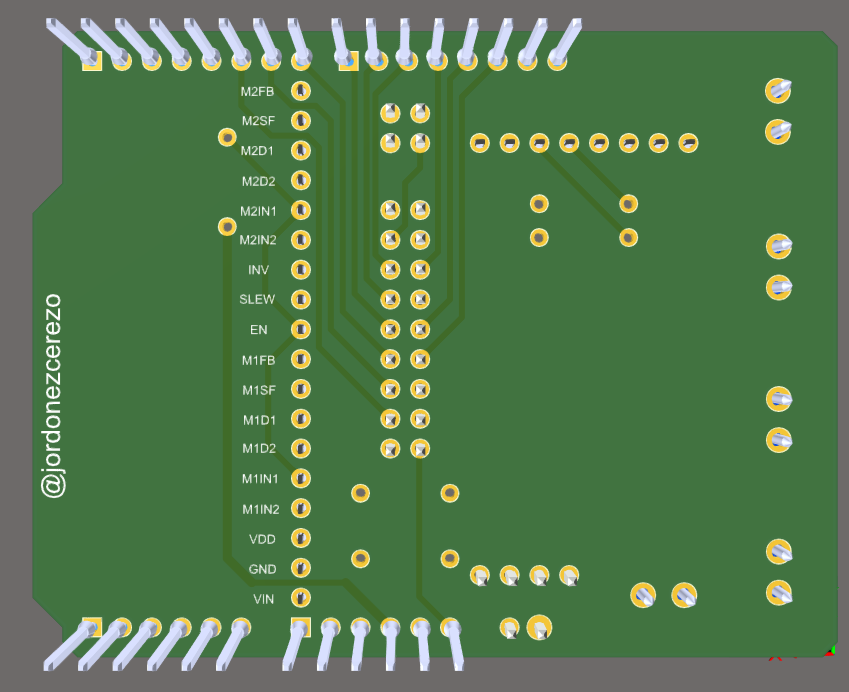
\includegraphics[scale=0.6]{imagenes/Balancing_Robot/bottom_3D.PNG}
			\caption{3D View of Shield for IceZum Alhambra II.}
			\label{fig:bottom_3D}
		\end{figure}
	\end{center}
	
	\begin{center}
		\begin{figure}[H]
			\center
			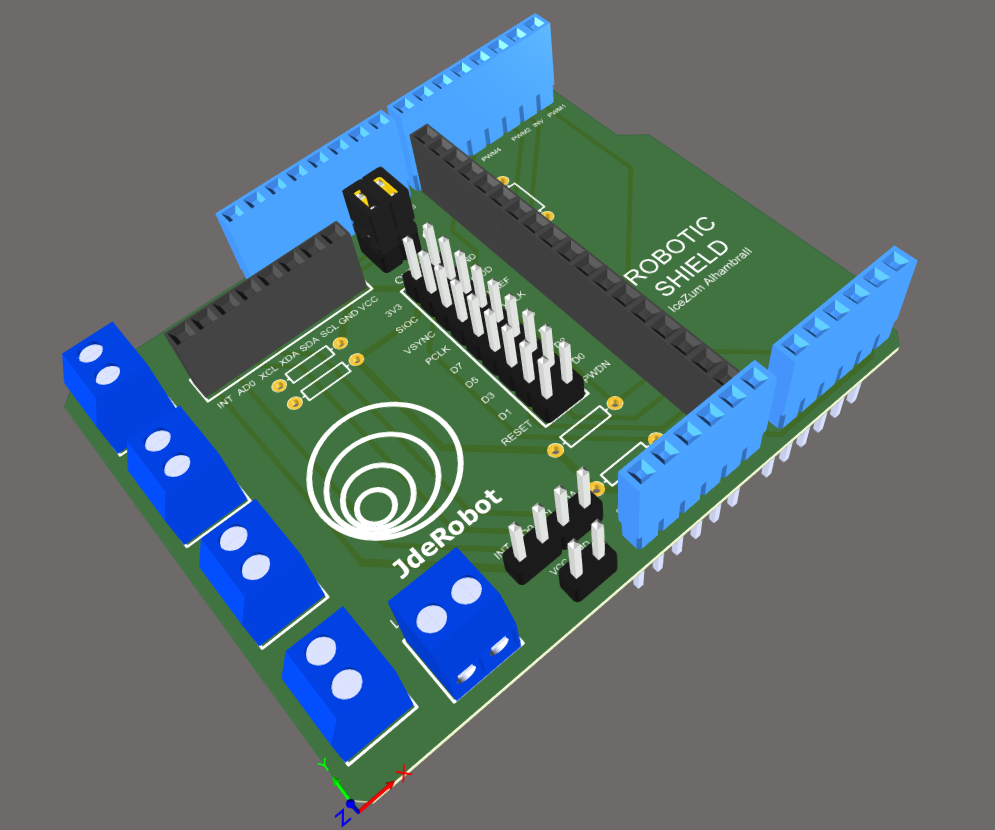
\includegraphics[scale=0.5]{imagenes/Balancing_Robot/Vista3D1.PNG}
			\caption{3D of shield for IceZum Alhambra II.}
			\label{fig:Vista3D1}
		\end{figure}
	\end{center}
	
	\begin{center}
		\begin{figure}[H]
			\center
			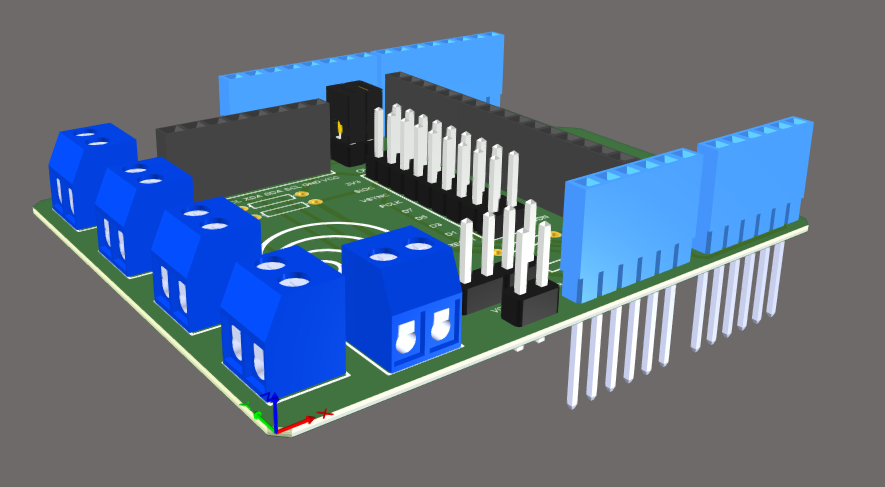
\includegraphics[scale=0.6]{imagenes/Balancing_Robot/Vista3D2.PNG}
			\caption{3D of shield for IceZum Alhambra II.}
			\label{fig:Vista3D2}
		\end{figure}
	\end{center}


For a PCB development with the described requirements it has been used Altium Designer. The elaboration process of a PCB in Altium can be different depending on the final user, but in this project the following root has been followed:

\begin{itemize}
	\item At first the project in issue is created.
	\item For each of the components used a new library is created, formed by the schematic and the layout in the PCB.
	\item Once all the libraries are created, the schematic of the plate is designed, taking special care that the connections are adequate.
	\item With the schematic already created, the PCB can be implemented defining its edges, tracks, pads, etc.
\end{itemize}

The scheme is represented in \ref{fig:schematics_tfg}.
\newpage

\begin{center}
	\begin{figure}[H]
		\center
		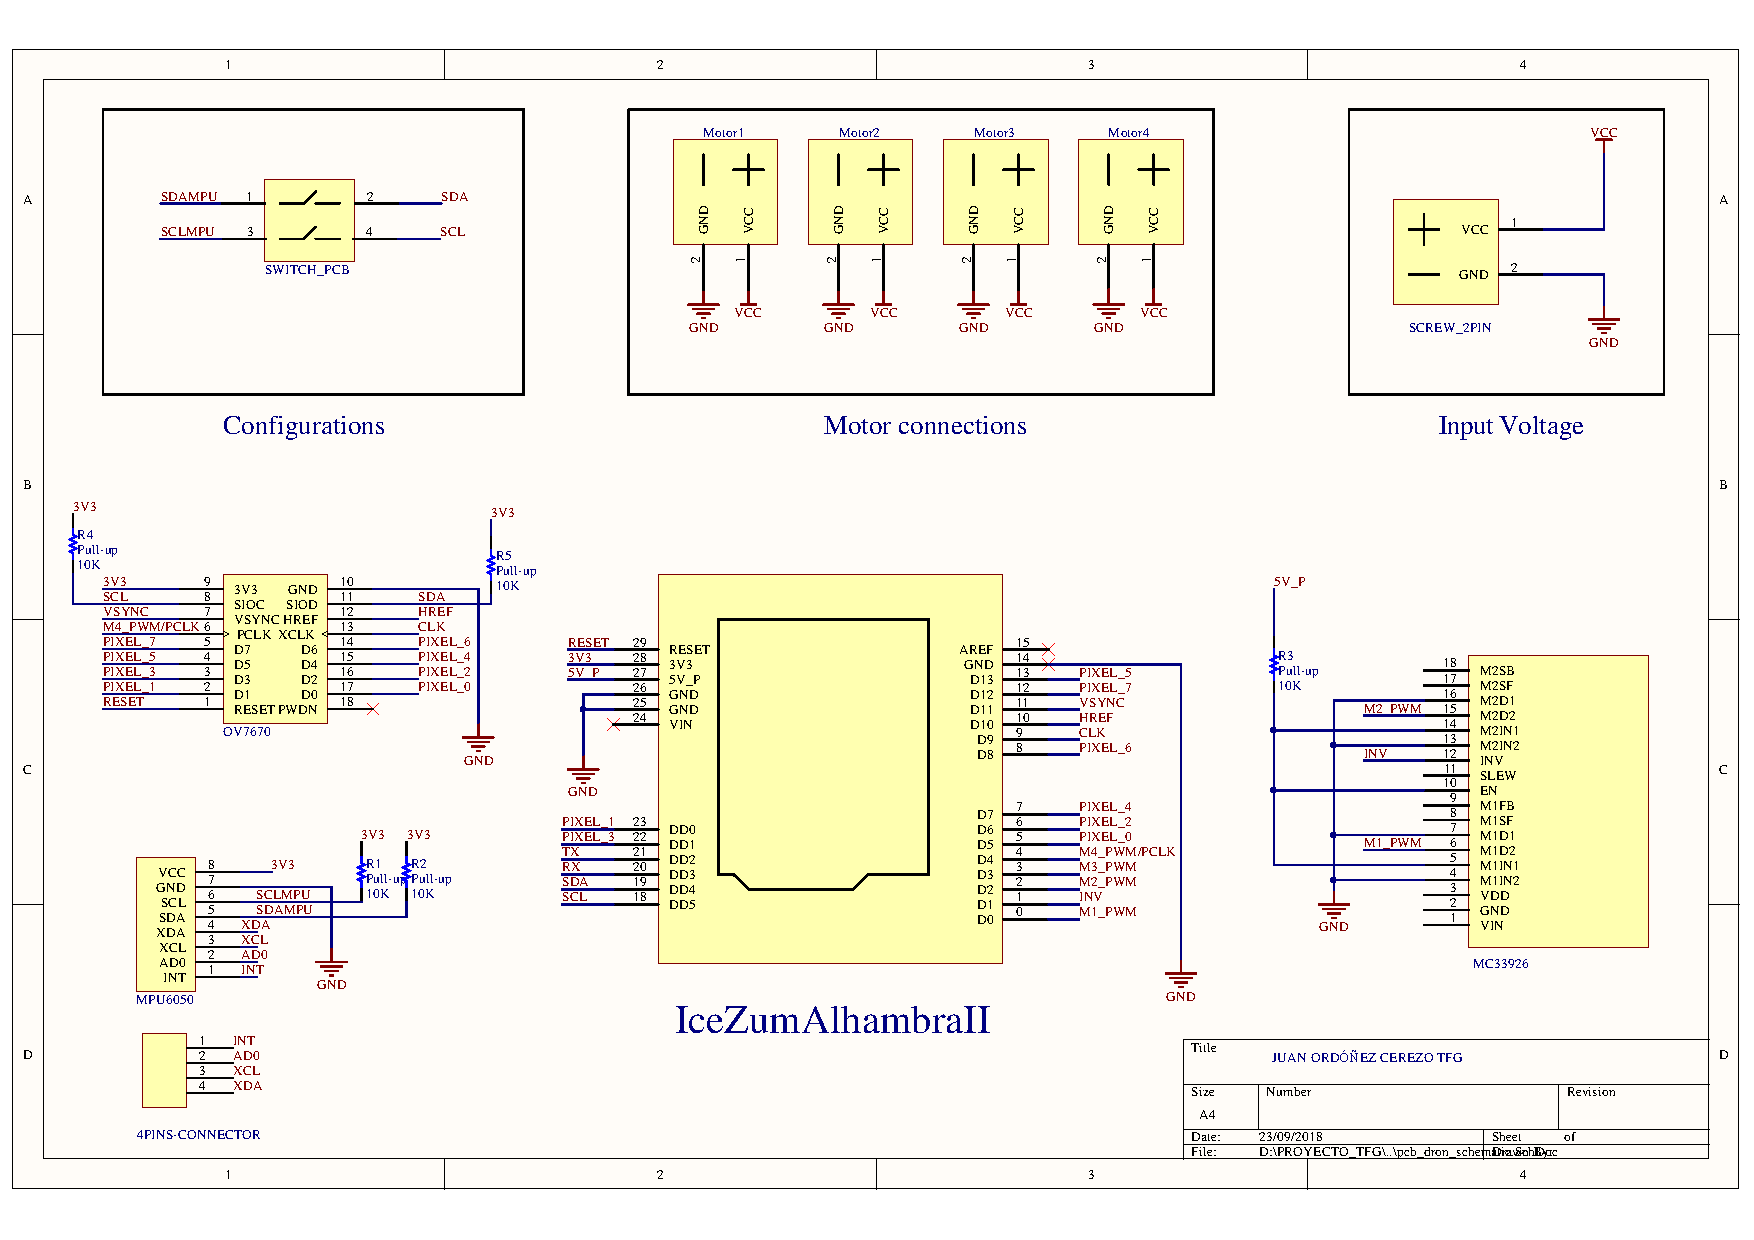
\includegraphics[scale=0.6, angle=90]{imagenes/Balancing_Robot/pcb_dron_schematic.pdf}
		\caption{Schematic Shield IceZum Alhambra II}
		\label{fig:schematics_tfg}
	\end{figure}
\end{center}
\newpage

\textbf{Trace size} \newline
When designing the PCB, the size of the copper trace should be considered, especially if the current could be very high. Otherwise, the PCB could suffer damage or even burn out. \newline

To calculate the trace width, it is necessary first to know the maximum intensity that could circulate through it. It is based on the knowledge that one of the engines of the unmanned aerial vehicle (this is the worst case and for which the calculation of tracks is necessary) can consume a maximum of 20 amps. This amount has been extracted from the datasheet and is usually common for this type of motors. \newline

The formula used to obtain the trace width has been extracted from the standar IPC-2221B, which establishes the generic requirements for the design of PCB.\newline

The formula is defined as in equation \ref{eqn:eqn31}: 

\begin{equation}
I = K * dT^{0.44}*(W*H)^{0.725}
\label{eqn:eqn31}
\end{equation}

Donde: 
\begin{itemize}
	\item I = Max. Intensity (A).
	\item dT =Temperature rise over ambient (Cº)
	\item W,H = With and Height (mils)
	\item K = 0.024 for internal traces and 0.048 for external traces.
\end{itemize}

The following results were obtained either for inner and outer traces:

\begin{equation*}
W_{externas} = 18.716 mm 
\end{equation*} 
\begin{equation*}
H_{externas} = 	0.035 mm
\end{equation*}
\begin{equation*}
W_{internas} =  48.6876 mm 
\end{equation*} 
\begin{equation*}
H_{internas} = 	0.035 mm
\end{equation*}

The thickness of the layer is provided by the manufacturer. In this project, this web has been used for ordering the PCBs. \newline 
Trace thickness is commonly measured in "oz" and in this case, the manufacturing company allows a 1oz trace thickness in a PCB with, which is equal to a 0.035mm thickness.\newline
If the results obtained from equation 3.1 are analyzed, the difference between a track in an inner layer and a track in an outer layer is clearly seen.\newline
A PCB is divided into layers, each of the layers has its function and organizing them properly is a good practice to avoid bad behavior. Thus, once the requirements were analyzed, two layers were necessary for the connection of data pins, in addition a ground plane is always recommended in which all the pins connected to GND have a common layer. This avoids noise and interference besides ensuring a good ground reference. \newline
In the used PCB provider, there is no price difference between a three-layer PCB and a four-layer PCB and considering that in the best case the trace width for the brushless motors should be of 1.8716cm, it was reached the determination of the usage of one of the layers as a common plane for the powering traces of the motors. The distribution of the layers would therefore be represented in Table \ref{tabla:layers_altium}.

For the rest of data traces, it is assumed a width of 20 mm, which allows a 1.46 A current, enough for this application.


\renewcommand\tablename{Table}
\begin{table}[H]
	\centering
	
	\begin{tabular}{|l|l|}
		\hline
		Top Overlay           & Overlay              \\ \hline
		Top Solder            & Solder Mask/Coverlay \\ \hline
		\textbf{Top Layer}    & Signal               \\ \hline
		Dielectric 1          & Dielectric           \\ \hline
		\textbf{VCC}          & Signal               \\ \hline
		Dielectric 2          & Dielectric           \\ \hline
		\textbf{GND}          & Signal               \\ \hline
		Dielectric 4          & Dielectric           \\ \hline
		\textbf{Bottom Layer} & Signal               \\ \hline
		Bottom Solder         & Solder Mask/Coverlay \\ \hline
		Bottom Overlay        & Overlay              \\ \hline
	\end{tabular}
	\caption{Layers composition in PCB.}
	\label{tabla:layers_altium}
\end{table}



A 2D image of the Top Layer, VCC, GND, Bottom Layer, Top Overlay and Bottom Overlay layers are shown in Figure \ref{fig:layers_altium}.


\begin{center}
	\begin{figure}[H]
		\center
		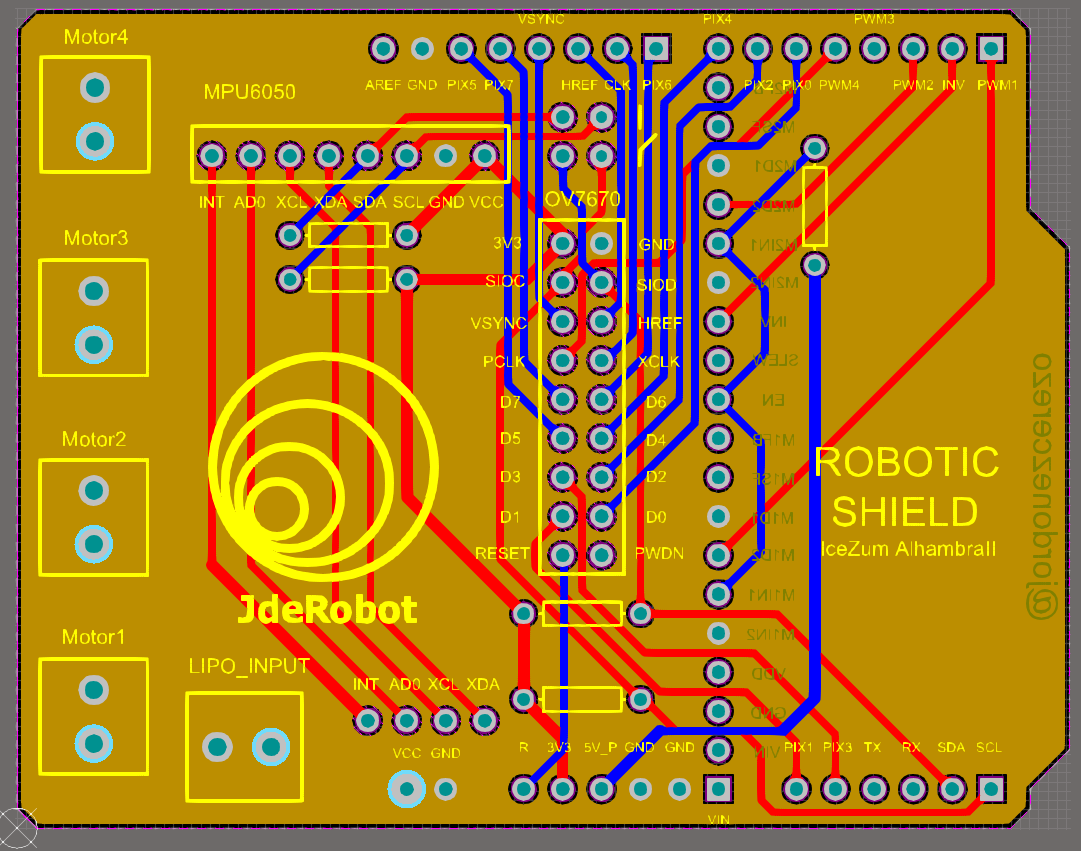
\includegraphics[scale=0.4, angle=90]{imagenes/Balancing_Robot/layers_altium.PNG}
		\caption{Composition layers in Altium.}
		\label{fig:layers_altium}
	\end{figure}
\end{center}


\subsection{IceZum Alhambra-Arduino Nano Implementation}\label{sec:Integracion}

An integration between a microcontroller and FPGA allows to distinguish sequential and parallel tasks, assigning each process to the microcontroller if it necessarily has to be sequential, or to the FPGA if the process can be parallelized and obtain with it some advantages\newline

There are some options to make a Microcontroller/FPGA integration:

\begin{itemize}
	\item Emulate the behavior of a microcontroller in an FPGA.
	\item Physical coexistence of an FPGA and microcontroller creating a communication between each one of them.
\end{itemize}
In this project the second one has been chosen as an option because there are not enough resources to carry out the first one, although this would be the most adequate in terms of saving resources and ease of use. \newline

There are two possible communication types to this purpose:
\begin{itemize}
	\item Serial communication: It is a sequential communication. The bits are sent one by one, sequentially and using only one data bus.
	\item Parallel communication: All bits of each symbol are sent at the same time.
\end{itemize} 

To make usage of the communication in parallel you need as many channels as bits to have the information to be transmitted (if you want to send a byte you should use a total of 8 channels, corresponding to each bit). In this case there will be used 8 pins of the FPGA to be able to carry out this type of transmission. Therefore, and despite the fact that parallel communication is quicker than serial communication, the first one is chosen as the most convenient option. \newline

The type of serial communication developed could be alike an SPI protocol, although it only has data capacity in one direction. The schematic of this developed communication is shown in Figure \ref{fig:coexistencia2}.

\begin{figure}[H]
	\center
	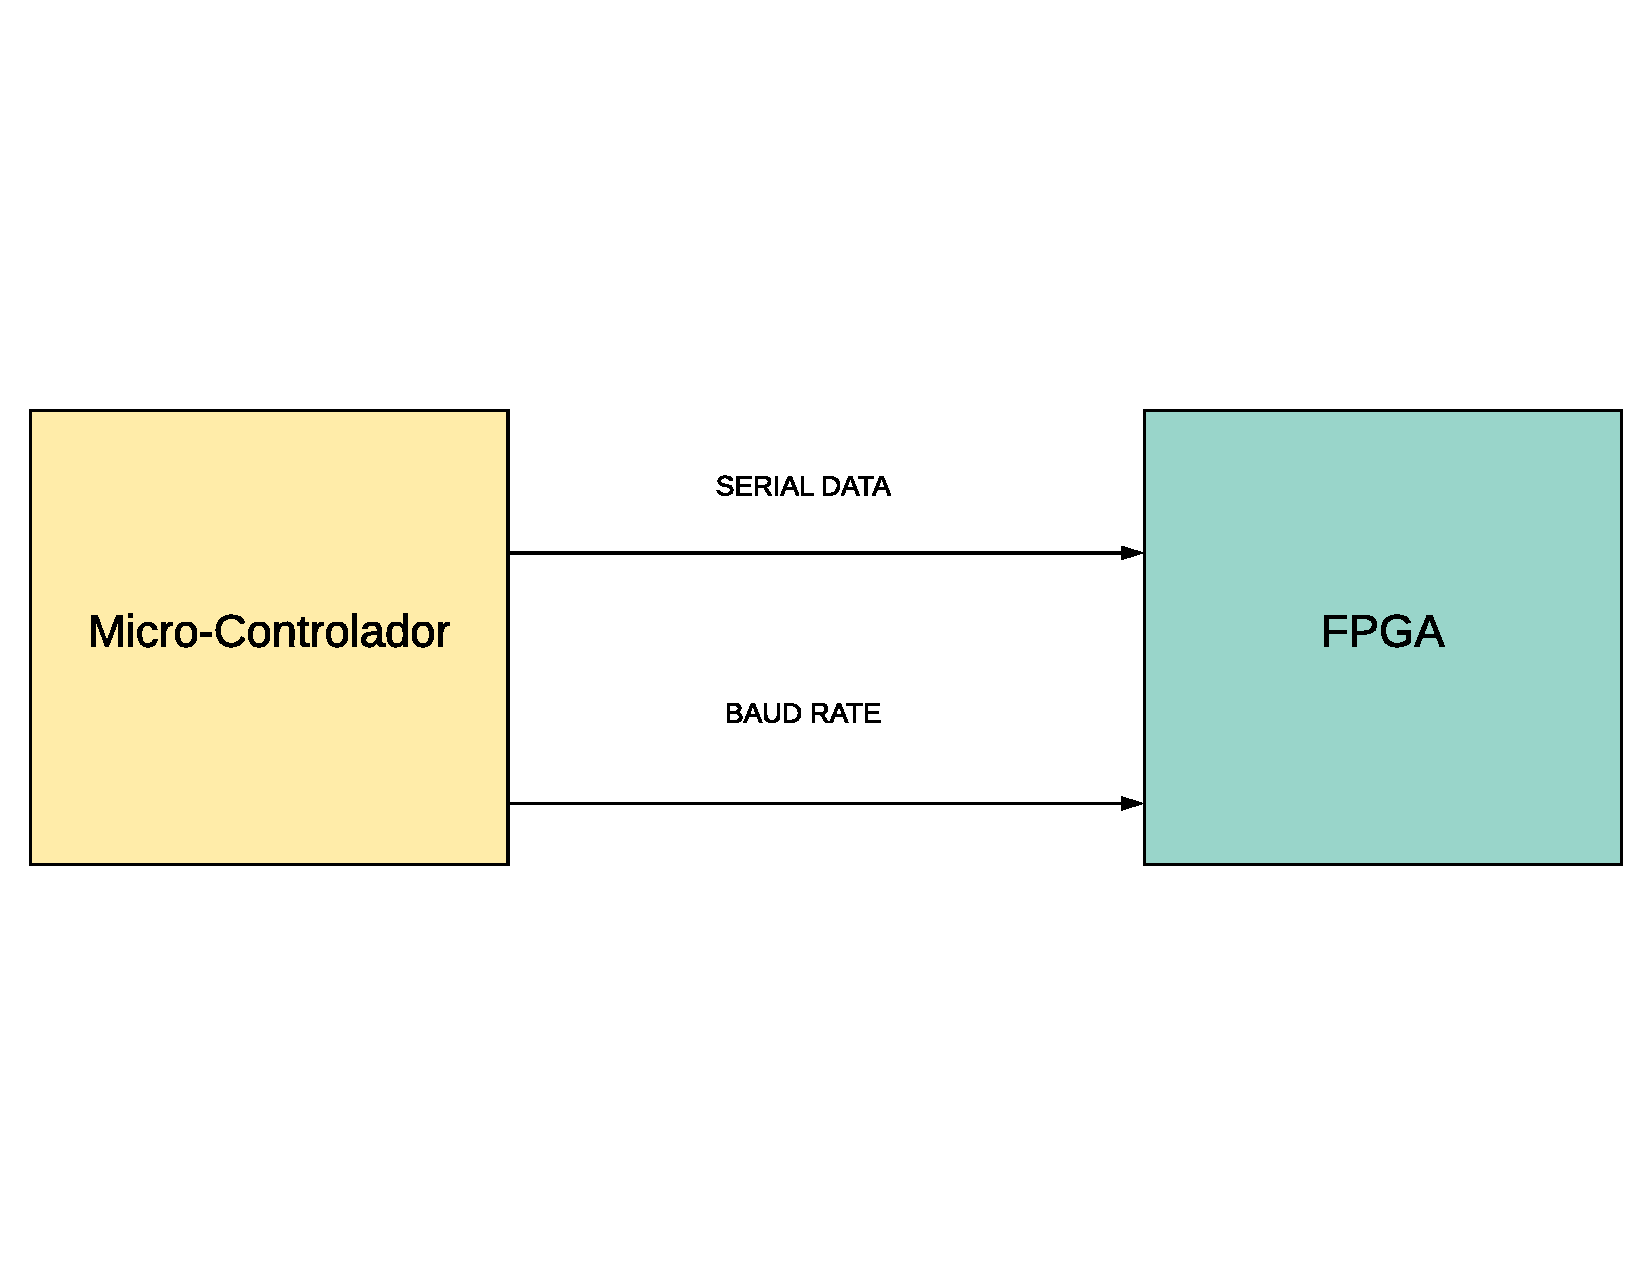
\includegraphics[trim = 0mm 40mm 0mm 20mm, clip,scale=0.4]{imagenes/Balancing_robot/coexistencia2.pdf}
	\caption{Hardware coexistence microcontroller-FPGA.}
	\label{fig:coexistencia2}
\end{figure}
The general system has two connections:
\begin{itemize}
	\item A data line to send the information.
	\item A clock line so that the FPGA could obtain at every time the information speed.
\end{itemize}

A possible example of a serial communication of a data byte could be shown in Figure \ref{fig:serial_comunicattion}. 

\begin{center}
	\begin{figure}[H]
		\center
		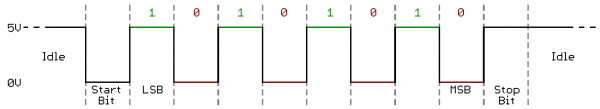
\includegraphics[scale=0.75, angle=0]{imagenes/Balancing_Robot/serial_comunicattion.png}
		\caption{Serial communication example.}
		\label{fig:serial_comunicattion}
	\end{figure}
\end{center}

The angle has to be known in the IceZum-Alhambra in order to make decision both in direction as in the speed of the engines. It is therefore necessary a microcontroller/FPGA communication (Figure \ref{fig:coexistencia1}).

\begin{figure}[H]
	\center
	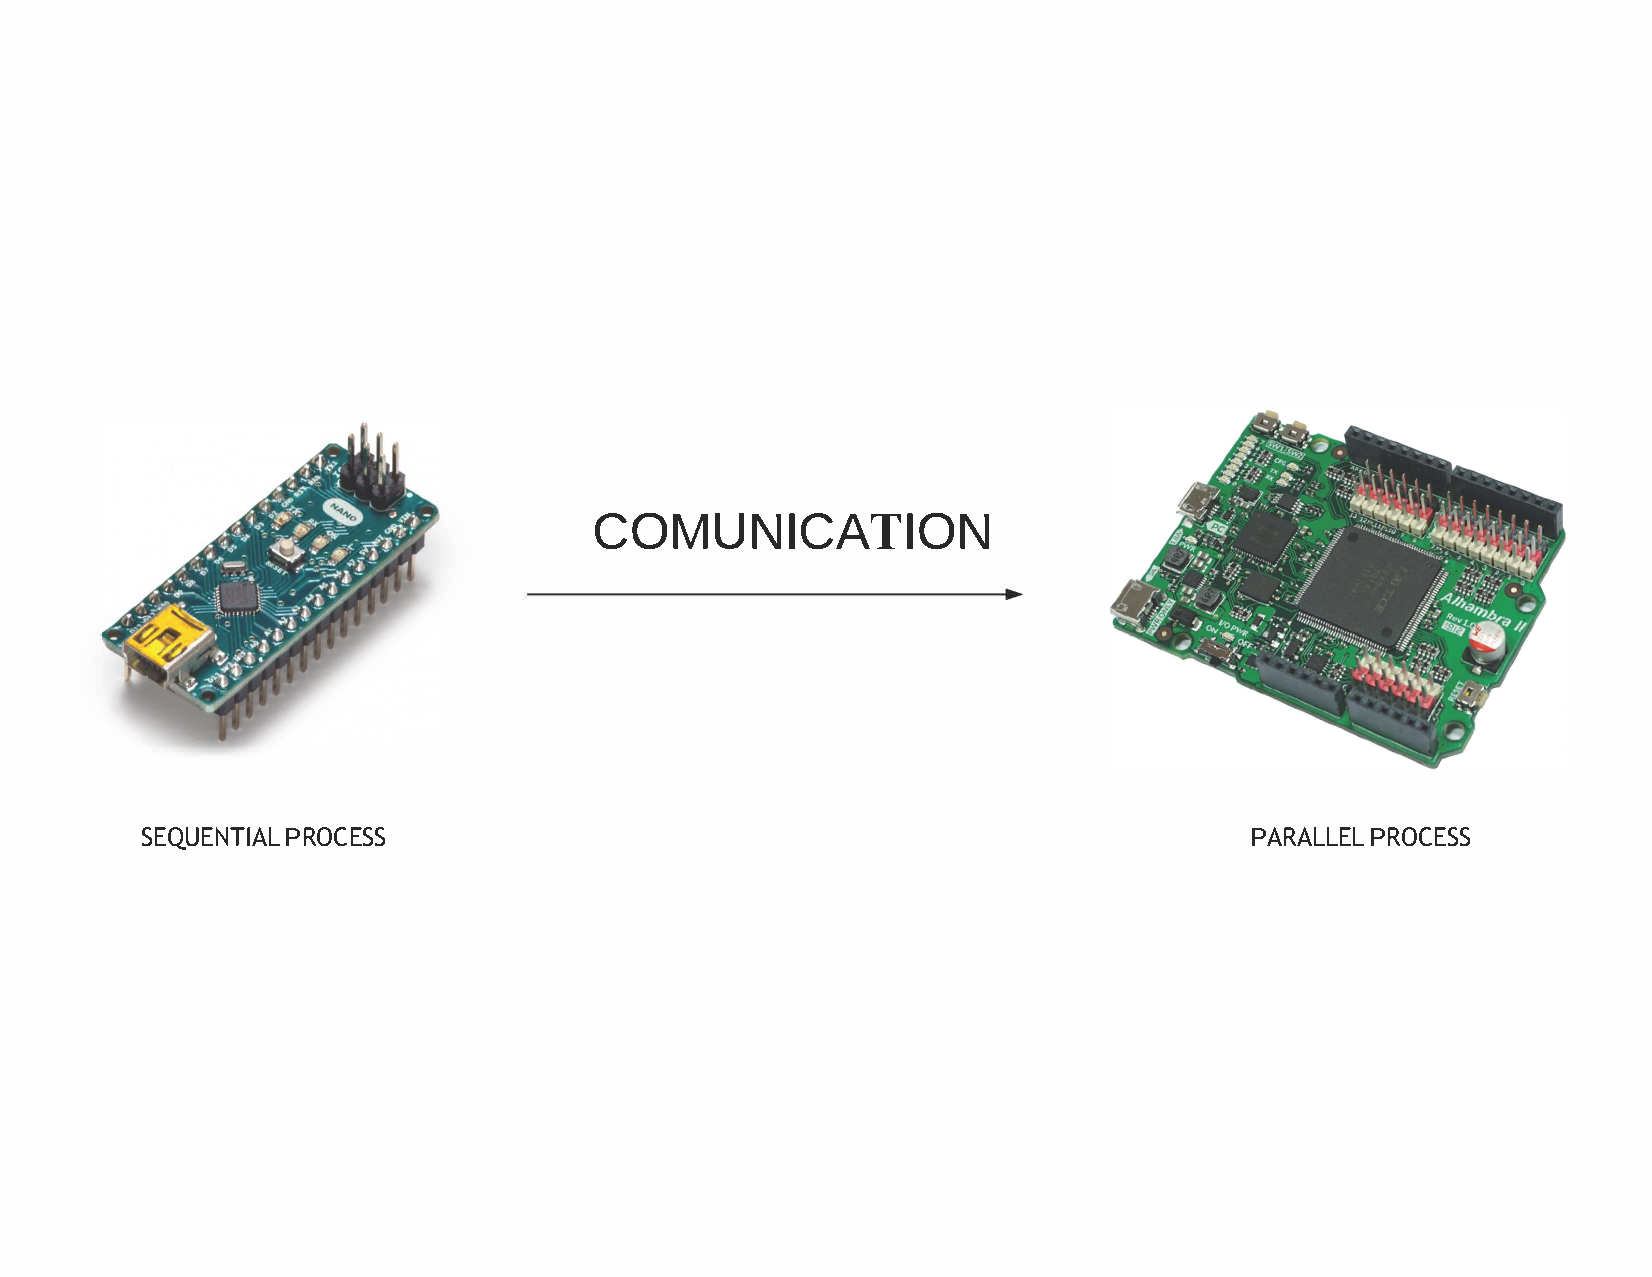
\includegraphics[trim = 0mm 40mm 0mm 20mm, clip,scale=0.4]{imagenes/Balancing_robot/coexistencia1.pdf}
	\caption{Separation microcontroller-FPGA.}
	\label{fig:coexistencia1}
\end{figure}

The communication would be only unidirectional, the microcontroller will send information to the FPGA about the current angle of the object in issue with the purpose that the FPGA analyzes and actuates starting from that angle.\newline

Therefore, there’s a two-part separation: from the point of view of the microcontroller and from the point of view of the FPGA. Both will be explained specifically in subsection \ref{sec:vista_controlador} y \ref{sec:vista_controlador}

\subsubsection{Microcontroller POV}  \label{sec:vista_controlador}

For the development of this sub-chapter, it is assumed that the current angle has already been obtained in the microcontroller. Thus, and for the clarity of the reader, an internal schematic of the Arduino Nano is shown in figure \ref{fig:coexistencia3}. In this section and according to the part of the microcontroller, only the shadowed part is analyzed. 

\begin{figure}[H]
	\center
	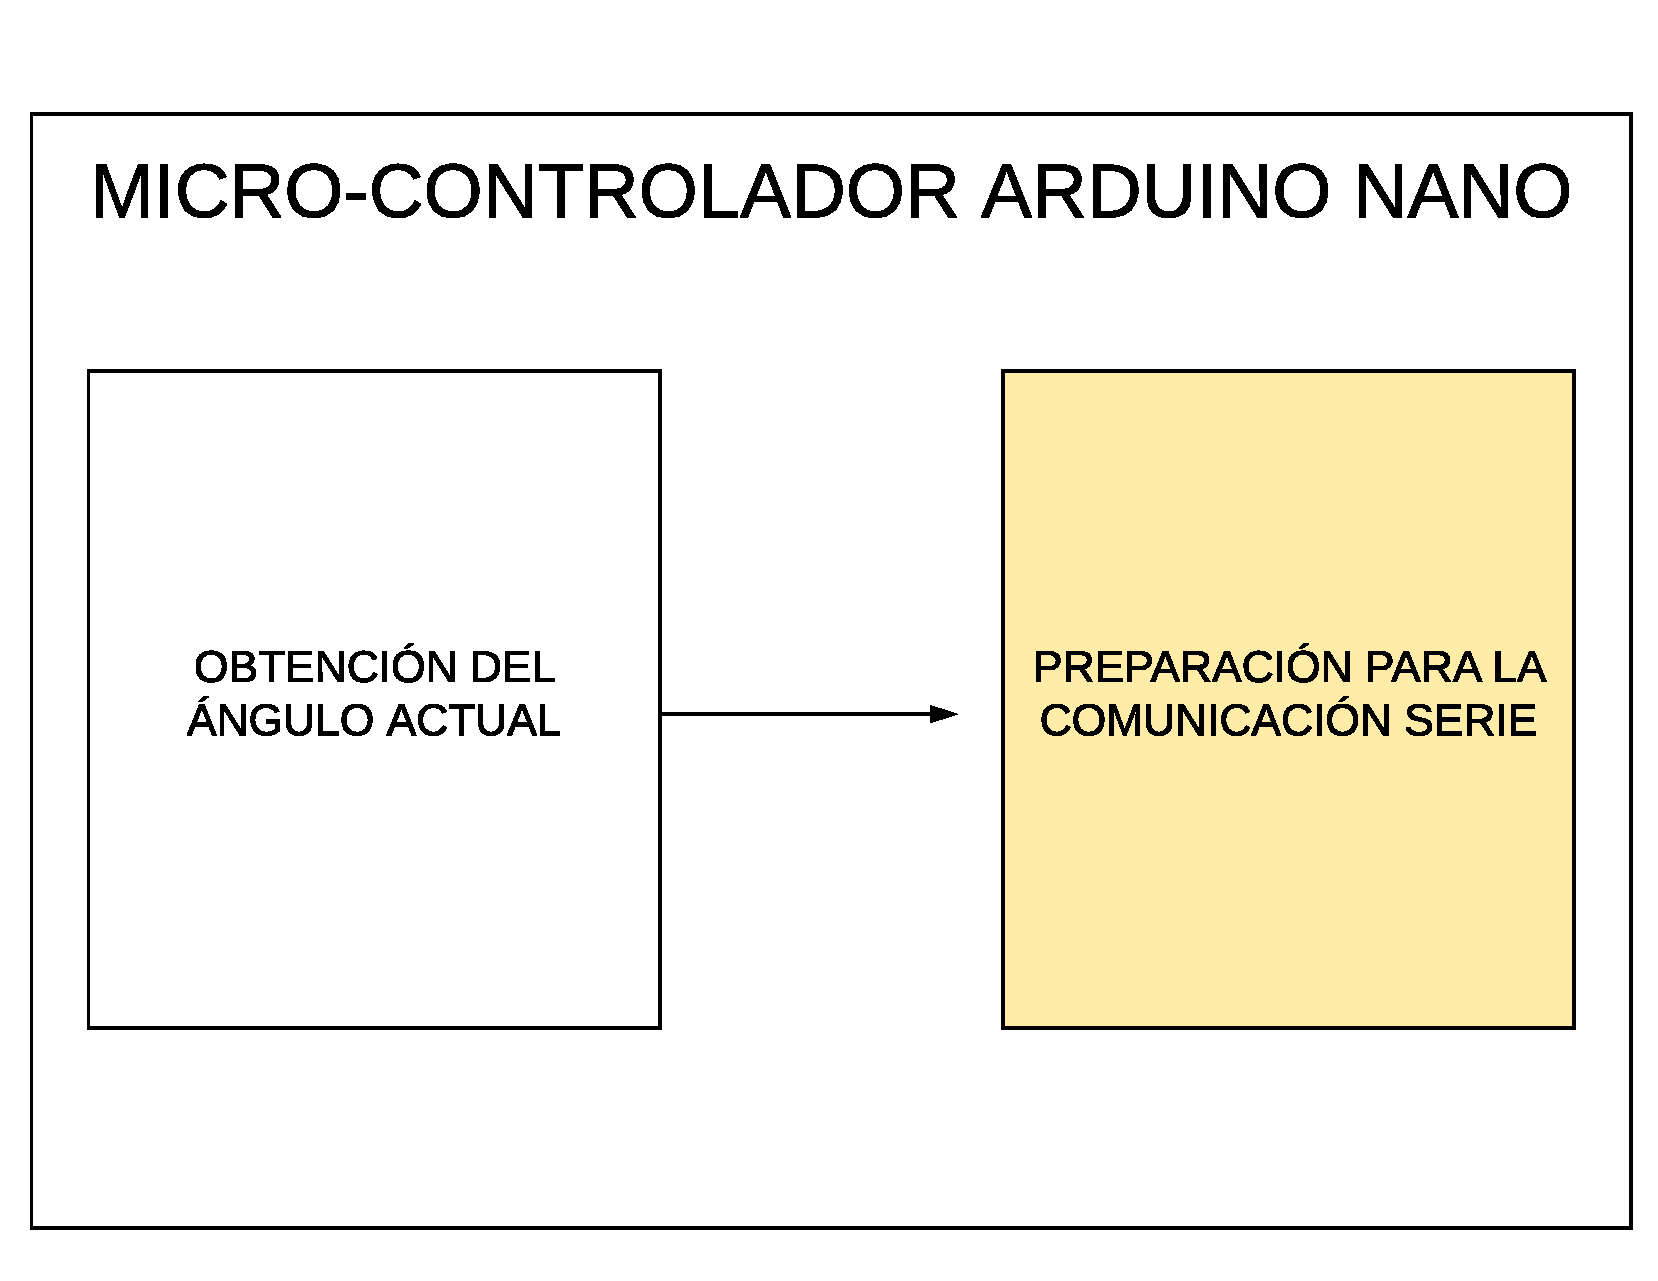
\includegraphics[trim = 0mm 0mm 0mm 0mm, clip,scale=0.3]{imagenes/Balancing_robot/coexistencia3.pdf}
	\caption{Inner diagram Arduino Nano.}
	\label{fig:coexistencia3}
\end{figure}

The flow diagram in which the C code of the microcontroller is based on, is shown in Figure \ref{fig:extraccion_angulo}.

\begin{figure}[H]
	\center
	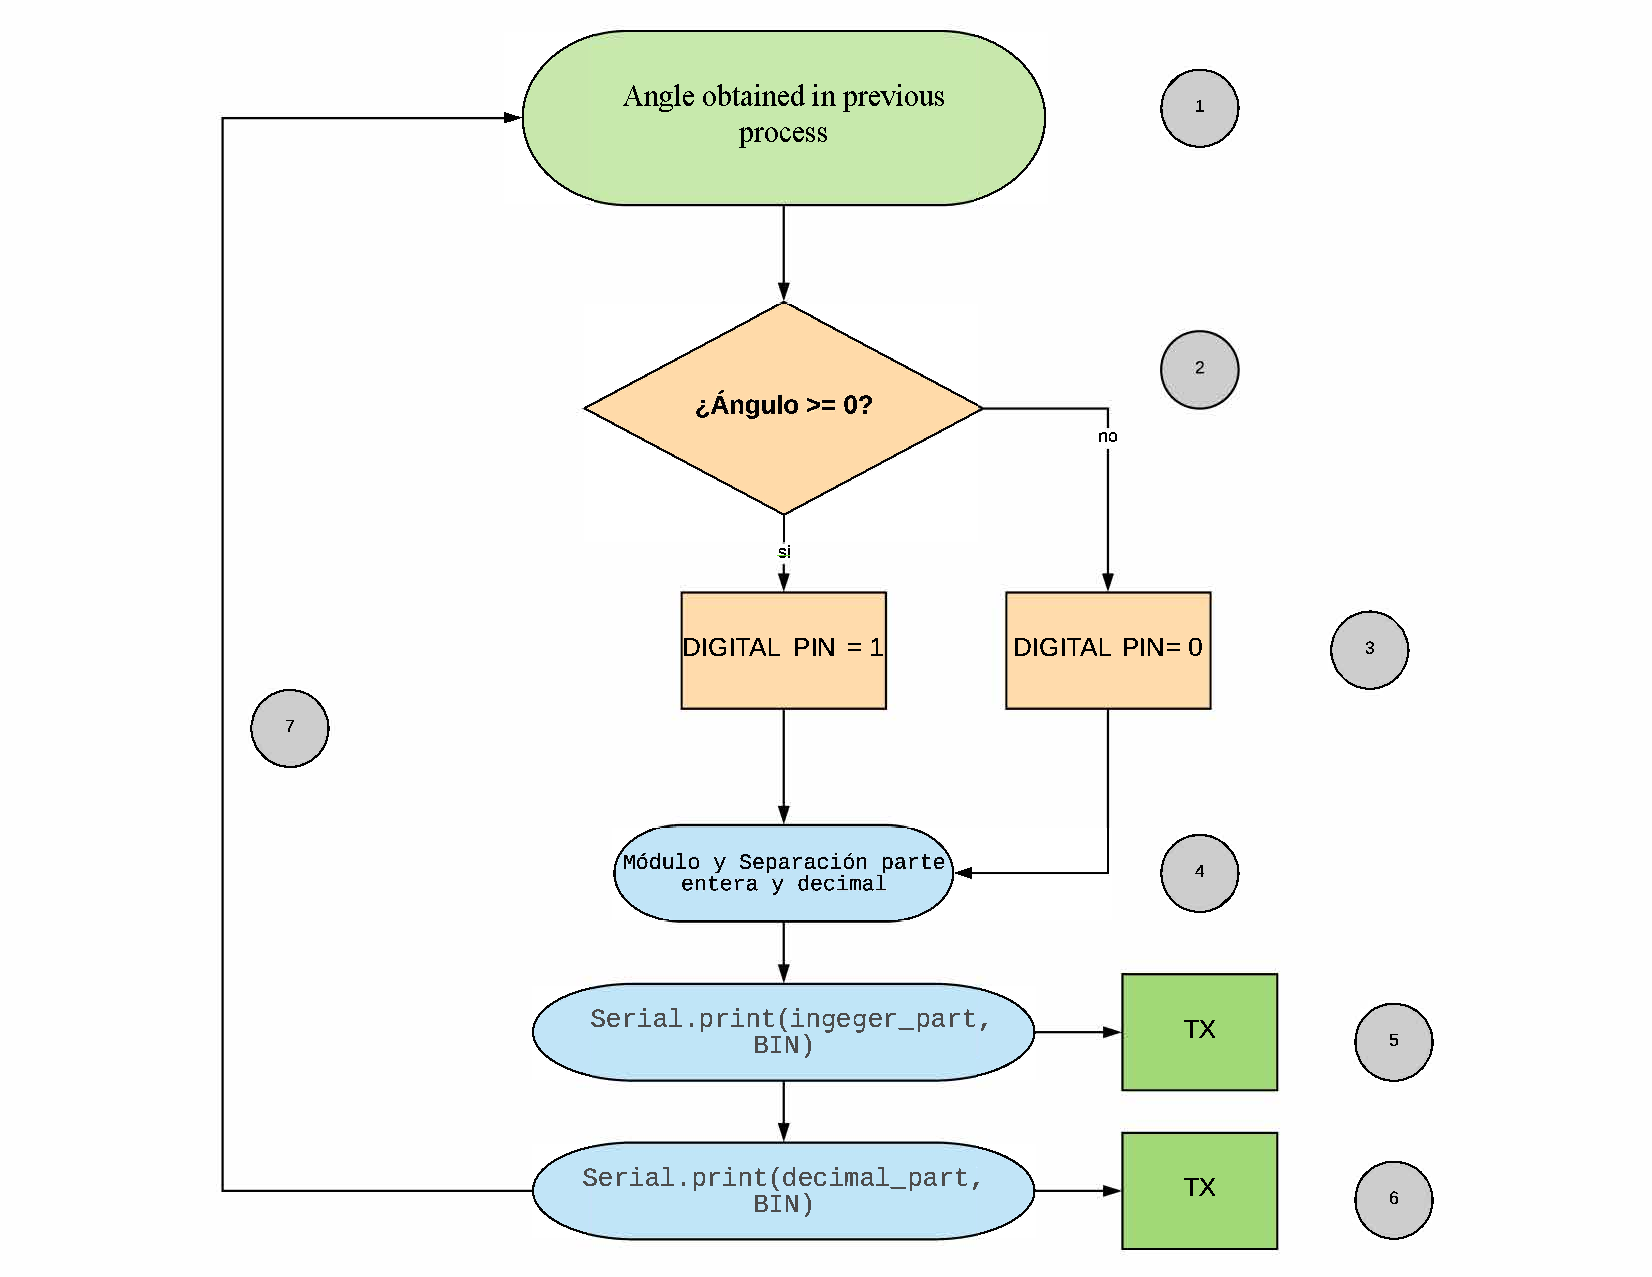
\includegraphics[trim = 0mm 0mm 0mm 0mm, clip,scale=0.5]{imagenes/Balancing_robot/extraccion_angulo.pdf}
	\caption{Flow diagram to send angle.}
	\label{fig:extraccion_angulo}
\end{figure}

The most relevant features will be explained: 

\begin{itemize}
	\item It is based on the assumption that the angle has already been obtained and is correct. In section \ref{sec:MPU6050} you can find more information about it.
	\item As it has been said before 3.3.2, one of the most important parts to correct the control of the self-balance robot, is to know the inclination at every moment to correct this desviation (\ref{fig:angle_correction}). To do this, the FPGA must know if the angle is positive or negative. This aspect would not form part of the communication protocol itself, as will be seen below. 
\end{itemize}
	
	\begin{figure}[H]
		\center
		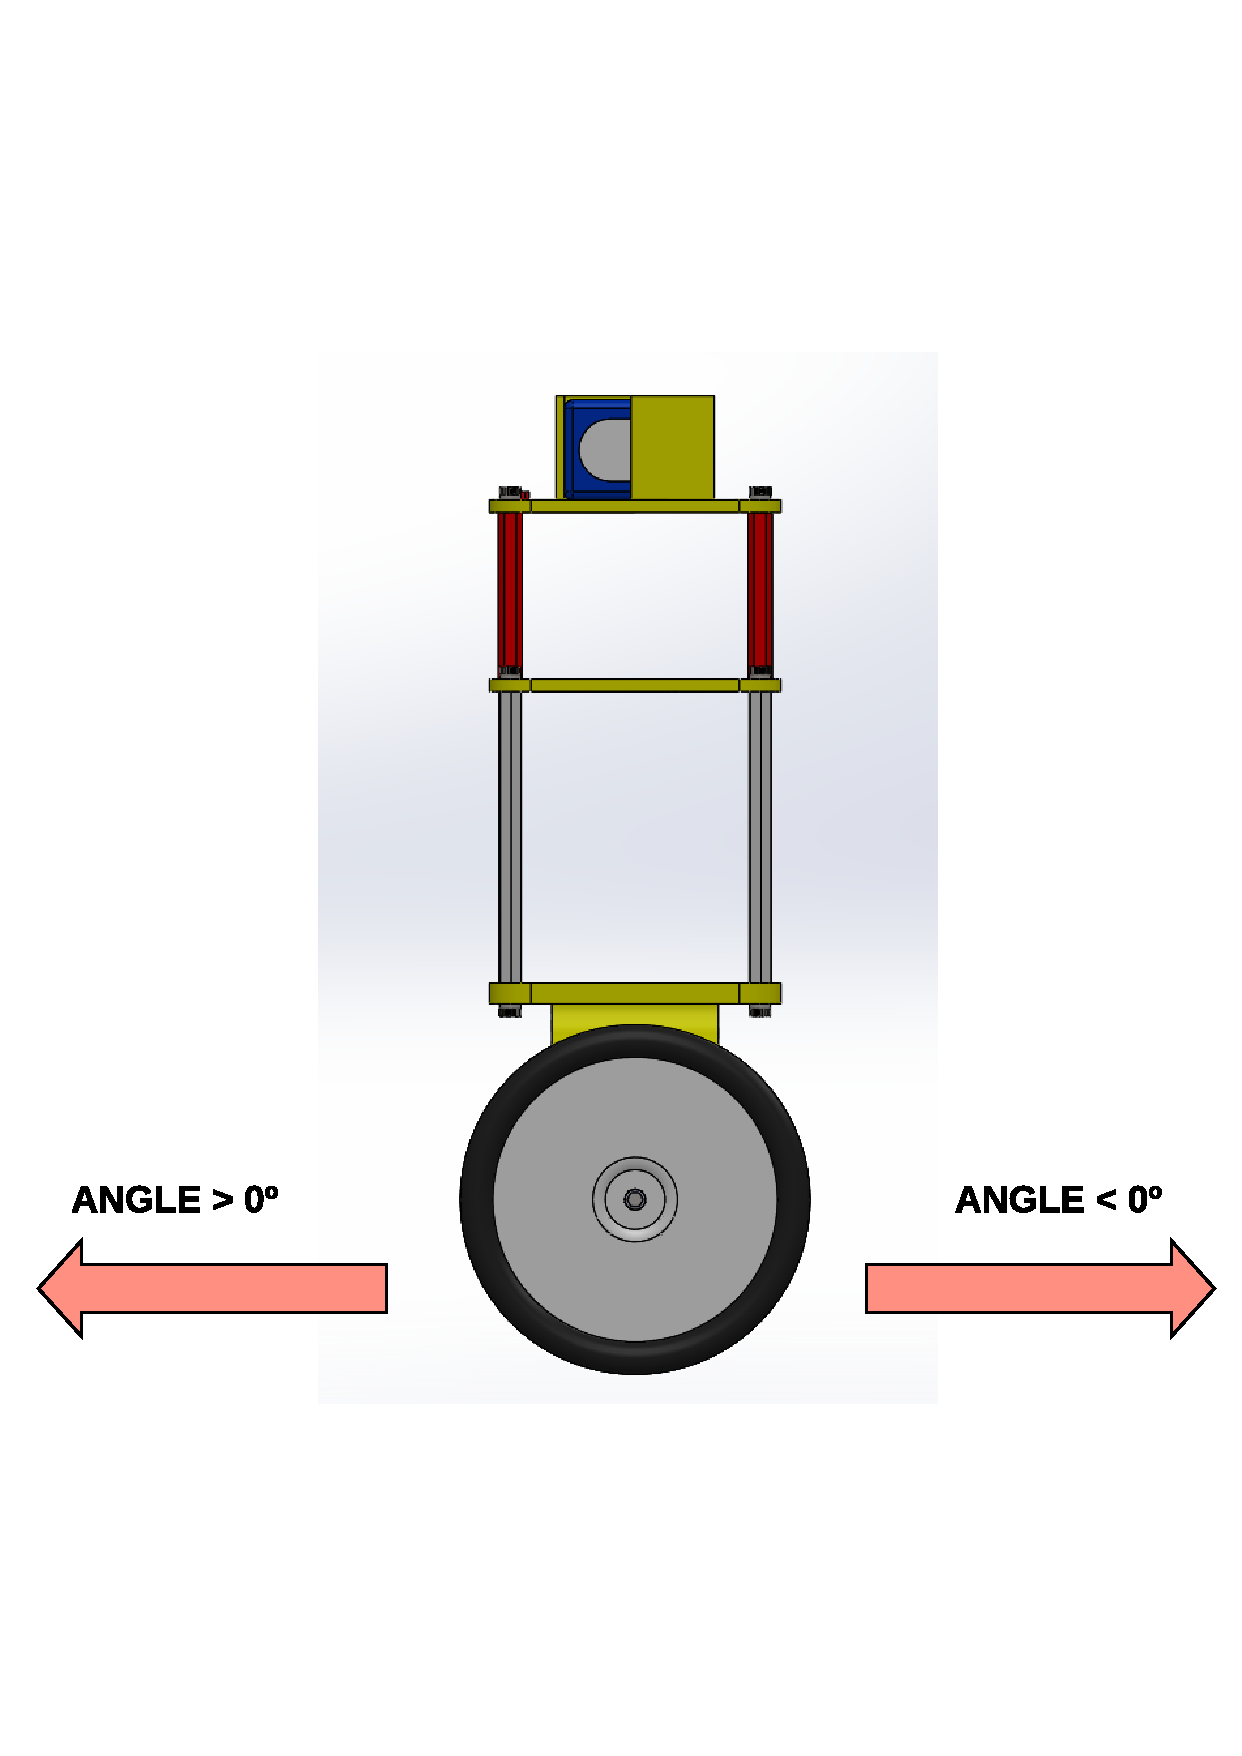
\includegraphics[trim = 0cm 4cm 0mm 4cm, clip,scale=0.5]{imagenes/Balancing_robot/angle_correction.pdf}
		\caption{Correction angle in Self-Balance Robot.}
		\label{fig:angle_correction}
	\end{figure}
	
\begin{itemize}	
	\item A single pin of the microcontroller is used, which will change its value to 1 or 0 depending on the sign of the angle at each moment. This way the FPGA will only have to read this information when it is necessary.
	
	\item For a correct understanding by the FPGA it is necessary to send the represented Angle in bytes and not in ASCII code. This is why for that sending the "Serial.print(Angle)" command will be used. This Arduino function sends by the serial port the representation in bytes of the angle in issue.\newline
	If the whole angle is intended to be sent, both the symbol and the ASCII code of the comma will be sent, and this is an aspect that does not matter to be considered when processing the FPGA is referred. To correct it, first the module of the angle is made (the sign is not needed because there is already a pin designated for it) and later it makes a separation between the integer and the decimal part in order to eliminate the "comma" character.
	\item The integer part corresponding byte is sent by the serial port.
	\item The decimal part corresponding byte is sent by parallel port.
	\item This is a loop that will be reproducing each “x” seconds, this is, the angle that could be corrected each “x” seconds. 
\end{itemize}


\subsubsection{FPGA POV} \label{sec:vista_fpga}

For an input PIN to the FPGA it will be continuously entering data from the transmission pin and so that it can make a correct reading of the byte it is necessary to know: 

\begin{itemize}
	\item When a byte transmission starts.
	\item When a byte transmission ends.
	\item When a bit can be captured. 
	\item When the necessary bits are saved in a buffed until the byte is complete.
\end{itemize}

In order to implement an intermediate module in the FPGA with the previous features (aspect in IceStudio Figure \ref{fig:arduino_interface}) it is necessary previously know the speed of the transmission by the microcontroller, which has been 16200 baud. \newline


\begin{figure}[H]
	\center	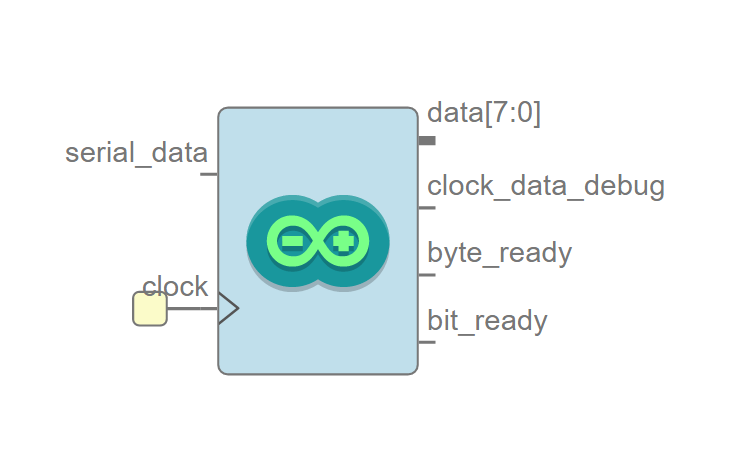
\includegraphics[scale=0.6]{imagenes/Balancing_robot/arduino_interface.PNG}
	\caption{Appearance of 	Arduino Nano module in IceStudio.}
	\label{fig:arduino_interface}
\end{figure}

The inputs and outputs from the previous module are detailed:

\begin{itemize}
	\item data[7:0]:Consists in a buffer in which bits are being stored when it is necessary until we have the byte. It is important that the following module knows when the byte is prepared for its capture.
	\item clock\_data\_debug: The usage of this output is for depuration only.
	\item byte\_ready: A clock flag will change its state when a byte is ready to be captured. As there has been seen in previous developments, this byte will be both integer or decimal part.
	\item bit\_ready:The usage of this output is for depuration only.
\end{itemize} 

The implementation in IceStudio of the previous behavior is implemented by two machine states with their corresponding sensitivity lists and the flow diagram is represented in Figure \ref{fig:arduino_interfacefluid}.

\begin{center}
	\begin{figure}[H]
		\center
		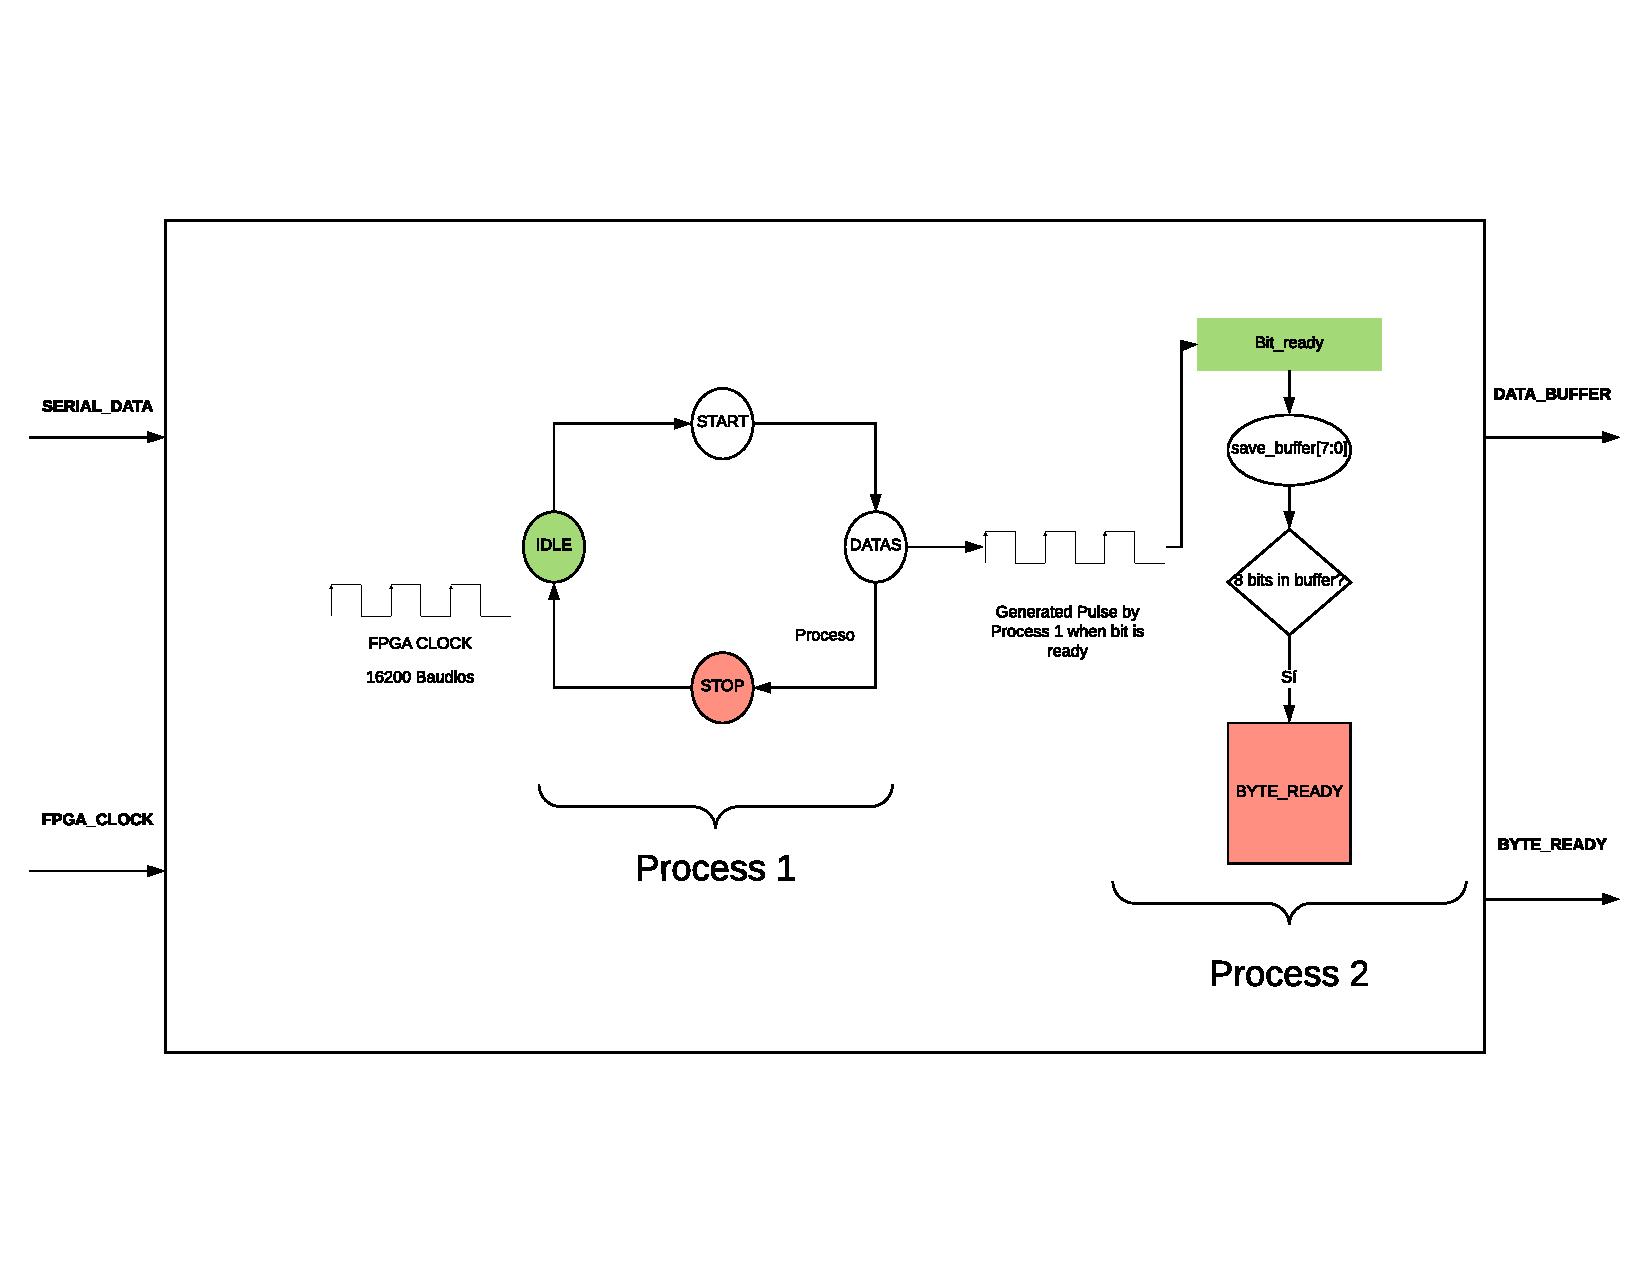
\includegraphics[trim = 0mm 0mm 0mm 10mm, clip,scale=0.7, angle=90]{imagenes/Balancing_robot/arduino_interfacefluid.pdf}
		\caption{Flow diagram for Arduino interface.}
		\label{fig:arduino_interfacefluid}
	\end{figure}
\end{center}

 Two well differenced processes are used:\newline
\textbf{Process 1:} This process only gives the next system the exact moment at which it can
capture a bit and save it in the buffer, for this, you must know the speed of the transmission discussed above. The states would be the following:

\begin{itemize}
	\item IDLE: The process remains in this state until the transmission starts, which will go to the next state (START).
	\item START: How was it developed in the section … The serial transmission protocol begins with a start condition, this state will allow to recognize when this condition ends to start saving bits in the buffer. 
	\item DATA: Since the transmission speed is already known and the condition of START in the previous state has been recognized, in this state a flag will change its value
	when the bit is ready to be stored in the buffer, of which process 2 will be in charge of.
	\item STOP: In addition to a START condition, the serial transmission protocol used in Arduino has a STOP condition. This state allows to recognize the time it takes Arduino to carry out this last condition, then, it will return to the first state until a new transaction begins.
\end{itemize}

\textbf{Process 2:} This process activated by process 1. When process 1 determines that a bit is available on the bus to be captured, it will set a clock flag on, initiating process 1 through a sensitivity list. The flow diagram could be:

\begin{itemize}
	\item Wait until the sensibility list is activates, this will indicate that a bit could be captured.
	\item Bits will be storing in a buffer that will form a byte, which will represent the integer or decimal part of the angle at that moment.
	\item When the byte is prepared to be captured by two consecutive modules, a channel will be on, being available both the outputs and the buffer with the 8 bits and the channel "byte\_ready".
\end{itemize}

At this point the FPGA is able to differentiate when it can capture a byte (BYTE\_READY) and from where it has to capture the data bus (DATA\_BUFFER). However, an aspect that is not part of the communication itself, it is important to analyze if you want to get a correct operation. That is, if it has been previously said that the microcontroller continuously sends the integer and decimal part of the angle, if a good interpretation of this data is not made, it is possible that an angle on the FPGA is formed by a decimal part of an angle \textit{n} and the integer part of the angle \textit{n + 1}.  \newline

To do this, a module is created in IceStudio that is capable of ordering these values. The aspect of this module in IceStudio is shown in Figure 3.29. \ref{fig:arrange_arduino}.

\begin{figure}[H]
	\center
	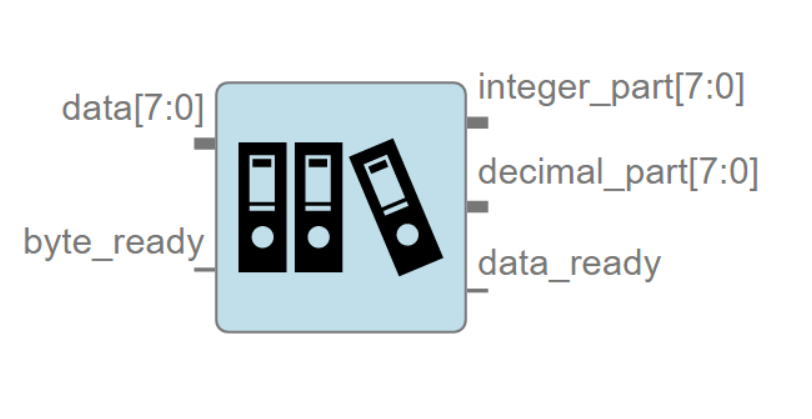
\includegraphics[scale=0.4]{imagenes/Balancing_robot/arrange_arduino.PNG}
	\caption{Module to arrange data from Arduino.}
	\label{fig:arrange_arduino}
\end{figure}

As Inputs there are:

\begin{itemize}
	\item Data [7:0]: This is the output buffer of the previous module where all captured bits are being stored until the byte is completed.
	\item byte\_ready : Clock flag which activates when the byte is available to be captured.
\end{itemize}

It is important to consider that the data will be available as long as the entire part as well as the decimal part of the angle in issue is available. Thus, as outputs are:

\begin{itemize}
	\item integer\_part[7:0] :Byte that represents the integer part of the angle.
	\item decimal\_part[7:0] : Byte that represents the decimal part of the angle.
	\item data\_ready : Clock flag that activates when the data (decimal and integer part) is waiting to be captured.
\end{itemize}

As has been previously discussed, the flow diagram of the code in Verilog that implements the previous behavior is shown in Figure \ref{fig:arrange_angle}.

\begin{figure}[H]
	\center
	\includegraphics[[trim = 0mm 4cm 0mm 4cm,clip, angle=0,scale=0.4]{imagenes/Balancing_robot/arrange_angle.pdf}
	\caption{Flow diagram to arrange bytes.}
	\label{fig:arrange_angle}
\end{figure}



In this case is a process with a sensibility list that counts as a sensible signal the "byte\_ready", bus and which is the output from the previous module. \newline

Each time the flag is activated that indicates that a byte Is ready to be captured, a cyclic state machine starts that counts with the following states:

\begin{itemize}
	\item DATA1: It is the first data to be captured and corresponds to the whole part of the first angle. The second time the "byte ready" flag is activated, it corresponds to the decimal part of the first angle and therefore it will pass to the next DATA2 state.
	\item DATA2: In this state not only is the decimal part of the angle in issue captured, but also a new flag is activated, which indicates that the complete data (Angle) is ready to be captured.
\end{itemize}

Thus, the module will have as outputs, the buffer of the integer part, the buffer of the decimal part and a bus that will notify the successive modules of the complete data is ready to be captured. In this way, the problem explained above of the non-ordering in the data arrived from the microcontroller has been avoided. \newline

The Arduino-FPGA communication protocol is terminated and the necessary tools are provided so that the successive processes and modules can know the angle at each moment represented by its integer part (8 bits), decimal part (8 bits) and a pin that indicates the value of the sign (positive or negative).

The final communication system between Arduino and IceZum Alhambra from a POV of the FPGA is represented in Figure \ref{fig:arduino_arrange}.

\begin{figure}[H]
	\center
	\includegraphics[scale=0.4]{imagenes/Balancing_robot/arduino_arrange.PNG}
	\caption{Communication between Arduino and IceZum Alhambra.}
	\label{fig:arduino_arrange}
\end{figure}


\newpage

\subsection{PID Control in IceZum Alhambra}
As it has been explained in section \ref{sec:PID}, a PID controller can be used in a simple way to control the stability of the system. \newline
One of the facilities in the use of this kinds of controllers is because its ease of implementation.
\subsubsection{P Controller} \label{sec:ControladorP}
The flow diagram that features the behavior of the P controller is shown in Figure \ref{fig:P_control}.
	\begin{figure}[H]
	\center
	\includegraphics[trim = 0cm 7cm 0mm 7cm, clip,scale=0.5]{imagenes/Balancing_robot/P.pdf}
	\caption{Flow diagram P control.}
	\label{fig:P_control}
\end{figure}

Due to its importance, the functionality is briefly explained ahead:

\begin{itemize}
	\item 1.-The complete process will be refreshed every time there is a new datum, this is in this case, every time the angle system is changing.
	\item 2.-As inputs there are both the integer part as the decimal part from the angle.
	\item 3.-Both the integer part and the decimal part are represented as 8 bits data without sign. So, in order to give more importance to the integer part, there is the option to divide the decimal part by 100 or to multiply the integer part by 100. In the first option there is not a good behavior obtained due to the digital treat of the floating comma, which is why the second option is better.
	\item 4.- At the end, the two integer and decimal components are added and then it is multiplied by a Kp constant, defined as a parameter which can be didactically changed.
\end{itemize}

Its representation in IceStudio has the aspect as shown in Figure \ref{fig:Pcontrol}.

\begin{figure}[H]
	\center
	\includegraphics[scale=0.5]{imagenes/Balancing_robot/Pcontrol}
	\caption{Appearance of P control in IceStudio}
	\label{fig:Pcontrol}
\end{figure}
\newpage
\subsubsection{D Controller} \label{sec:ControladorD}

Referring to the D controller, the flow diagram implemented in Verilog is shown in Figure \ref{fig:D_control}. 
	\begin{figure}[H]
	\center
	\includegraphics[trim = 0cm 0cm 0mm 0cm, clip,scale=0.4]{imagenes/Balancing_robot/D.pdf}
	\caption{Flow diagram D control.}
	\label{fig:D_control}
\end{figure}

Its implementation is composed by a state machine with two states, which will change at each pulse on the $data_ready$, which means, will change whenever a new angle is available.\newline

If remembered, D controller is based in its operation on the prediction of future errors. The derivative control action generates a control signal proportional to the derivative of the error signal. \newline
A subtraction (derived from the error in time) is therefore carried out between the current error and the last error. Its result is multiplied by the constant Kd. Its representation in IceStudio is represented in \ref{fig:Dcontrol}.

\begin{figure}[H]
	\center
	\includegraphics[scale=0.5]{imagenes/Balancing_robot/Dcontrol}
	\caption{Appearance of D control module in IceStudio.}
	\label{fig:Dcontrol}
\end{figure}

\subsubsection{Controlador PD}

Referring to the closed loop feedback system analyzed in section \ref{sec:PID}, it is important to show the final result of the aspect of the present project in IceStudio, making a direct comparison between this (figure \ref{fig:finalIceStudio} ) and figure \ref{fig:PID}.
\newpage
\begin{figure}[H]
	\center
	\includegraphics[scale=0.5, angle=90]{imagenes/Balancing_robot/finalIceStudio}
	\caption{Final appearance of Self-Balancin in IceStudio.}
	\label{fig:finalIceStudio}
\end{figure}

\subsection{Motor controller} \label{sec:driver_motores}
Having a module with the ability to generate PWM solves many subsequent problems while improving the visibility of the code in the final system. As can be seen in the motor features, most of them are commanded by a PWM signal that, although it is true, depends on the motor in issue. \newline
Pulse Width Modulation (PWM) is a technique that modifies the work cycle of a periodic signal (squared in our case) that is used to transmit information through a communication channel or to control the amount of energy that is sent to a load. An example of a PWM squared signal is shown in figure \ref{fig:pwm_example}.

\begin{figure}[H]
	\center
	\includegraphics[trim = 0mm 0cm 0mm 0cm, clip,scale=0.4]{imagenes/Balancing_robot/pwm_example.png}
	\caption{PWM signal example with different dutty.}
	\label{fig:pwm_example}
\end{figure}


Applying this signal, for example, to a classic DC motor the amount of energy that is applied to the load is varied, the motor in this case. It simply works as a switch in which a high logical level is open and a low level closed. If it is managed to vary the time the motor is being charged and the time in where there’s no current, you can control its speed. \newline

The features of a PWM signal are: 
\begin{itemize}
	\item D = Work cycle.
	\item $\tau$ = Time-lapse while the function is positive.
	\item T = Function period.
\end{itemize}


The motor driver used to control DC motors (MC3392 figure \ref{fig:driver_motor_fisico}),needs a series of configurations to work according to the needs which could be obtained from its datasheet. The final inputs and outputs diagram and also the necessary connections are detailed in the scheme of the \ref{fig:driver_motor} figure.


\begin{figure}[H]
	\center
	\includegraphics[trim = 0mm 0cm 0mm 0cm, clip,scale=0.4]{imagenes/Balancing_robot/driver_motor.jpg}
	\caption{MC33926 to control DC motors.}
	\label{fig:driver_motor_fisico}
\end{figure}


\begin{figure}[H]
	\center
	\includegraphics[trim = 0mm 3cm 0mm 2cm, clip,scale=0.4]{imagenes/Balancing_robot/driver_motor.pdf}
	\caption{Schematic MC33926.}
	\label{fig:driver_motor}
\end{figure}




\subsubsection{PWM Control}

The speed of the motors is controlled by a PWM which is connected to pin 15 or M2D2, from figure \ref{fig:driver_motor} for each one of the motors and another PWM generator connected to pin 6 or M1D1 from the DC motor driver. This generator module has the aspect shown in figure \ref{fig:pwm_module} in IceStudio. 

\begin{figure}[H]
	\center
	\includegraphics[scale=0.5]{imagenes/Balancing_robot/PWM_module.PNG}
	\caption{Appearance PWM module in IceStudio.}
	\label{fig:pwm_module}
\end{figure}

The block diagram of its performance is exposed in figure \ref{fig:pwm_control}.

\begin{figure}[H]
	\center
	\includegraphics[trim = 0mm 0mm 0mm 0mm, clip,scale=0.4]{imagenes/Balancing_robot/pwm_control.pdf}
	\caption{Flow diagram PWM generator in Verilog.}
	\label{fig:pwm_control}
\end{figure}

Its performance is based in an input clock pulse counter from the FPGA. A speed log will dictate how many pulses have to be counted before an output signal is settled on (desired PWM). As inputs are: \newline 
\begin{itemize}
	\item FPGA Clock: Is the 12Mhz FPGA clock which is in charge of the pulse counter.
	\item Start: It is a common signal to the whole system, performing as a switch to give a general start.
	\item Velocity: Is a record that marks how many clock pulses need to be counted before activating the output signal PWM.
\end{itemize}

As outputs are:
\begin{itemize}
	\item As outputs are:
\end{itemize}



\subsection{Power Supply System}


As with any electronic system, a power source is necessary to allow the correct operation of all the components. \newline

As a fundamental task, an analysis of the requirements of these components that make up the complete system is a priority in order to choose an adequate power supply. In addition, it is considered that the purpose is to have a mobile system and that, as far as possible, a direct connection to the electrical network or a USB connection to a computer is avoided. So, it only remains to choose what type of battery is suitable.\newline

Next, the different types of battery currently in the market are named, analyzing their most important advantages and disadvantages: 

\begin{itemize}
	\item Lead-acid Batteries: They are inexpensive and easy to manufacture but do not admit overloads or deep discharges, besides, they are heavy and have a big volume compared with the small amount of energy they are capable of storing.
	\item Nickel-cadmium Batteries (Ni-Cd): They work well over a wide range of temperatures and can be overloaded without damage. They allow deep discharges and provide a good number of cycles. As in the previous one, they have a very high weight and volume.
	\item Nickel-metal Hydride Batteries (Ni-MH): Features compared to the previous batteries are improved, however, it provides a fewer number of cycles.
	\item Lithium Ion Batteries (Li-ion): In comparison with the previous ones, these are from a recent development and have facilitated the existence of portable technologies. They have a high capacity in relation to their weight and volume, they have a very high self-discharge factor. They are almost unaffected by the
	memory effect and can be charged without having been previously discharged. On the other hand, they do not support temperature changes too good.
	\item Lithium Polymer Batteries (Li-Po): They are a variation of the Li-ion batteries that improve their weight and volume features as its discharge rate. They remain practically unused if they are discharged in excess.
\end{itemize}

Considering that the final and most restrictive system is a remotely piloted aerial vehicle, and that the self-balance robot needs a not very high weight, it is important that the weight features, volume, and discharge are adequate. For this reason, Li-po type batteries are chosen for the power supply of the systems in this project, which can store a large amount of energy and offer a very high discharge rate. \newline

The Li-Po type batteries have a different nomenclature from the rest, which is necessary to analyze:

\begin{itemize}
	\item Sort by number of cells "S": The number S corresponds to the number of cells, which are 3.7 volts but can reach 4.2 if they are fully charged. A 3-cell (3S) battery is composed of 3 sub-batteries placed in series, which is, a total of 11.1 volts.
	\item Capacity indicated in "mAh”: The higher the number of mAh, the higher the load capacity. A common mistake is to think that the greater the capacity, the greater the possibility of lengthening the time of the system in issue. At higher capacity, weight and volume of the battery increase, so the best configuration for this system must be found.
	\item Download rate "C": The number from C corresponds to the battery discharge rate. If a battery is 1C, it means that the maximum discharge rate it can reach is the one corresponding to its capacity. If the number C is different from 1 means that we multiply the discharge rate by that value, reducing the discharge time proportionally, that is, a battery of 1000mAh 2C will be discharged to 2A in half an hour.
\end{itemize}

The following approach will be to choose which of the previous values is the most adequate for the system. For this and after analyzig the differents components separately, two independent subsystems are distinguished in terms of the power supply:

\begin{itemize}
	\item DC Motors and Arduino Nano Power Supply.
	\item IceZum Alhambra II and other components Power Supply.
\end{itemize}

\subsubsection{DC Motors and Arduino Nano Power Supply}
For the DC motors and Arduino Nano power supply, a 11.1V and 2200mAh LIPO battery of is used as in figure \ref{fig:lipo111}. As it is presented in the final schematic from the controller
shield (Figure \ref{fig:schematics_tfg}), the battery is connected to the shield, which is in charge to supply both the motors and Arduino Nano.

\begin{center}
	\begin{figure}[H]
		\center
		\includegraphics[scale=0.8]{imagenes/Balancing_Robot/LIPO111}
		\caption{LIPO Battery 11.1V y 2.2A. }
		\label{fig:lipo111}
	\end{figure}
\end{center}

\subsubsection{Alhambra IceZum II and other components Power Supply}

For the IceZum Alhambra II power supply and the rest of the components, a 3.7V and 4mAh LIPO battery has been used, as shown in Figure \ref{fig:lipo37}. 
\begin{center}
	\begin{figure}[H]
		\center
		\includegraphics[scale=0.5]{imagenes/Balancing_Robot/LIPO37}
		\caption{LIPO Battery 3.7V y 4mAh.}
		\label{fig:lipo37}
	\end{figure}
\end{center}
\newpage
\subsection{Materials and Prototype Cost}
In the table \ref{tabla:coste} the total cost of the prototype along chapter \ref{sec: BalancingRobot} is pulled apart.
It is differenciated by four columns called material, number of units, unit cost and total cost in euros.
\begin{table}[H]
	\scalebox{0.9}{
	\begin{turn}{90}
	\begin{tabular}{|l|l|l|l|l}
		\cline{1-4}
		\multicolumn{1}{|c|}{\cellcolor[HTML]{FFCE93}\textbf{MATERIAL}} & \cellcolor[HTML]{FFCE93}\textbf{QUANTITY} & \multicolumn{1}{c|}{\cellcolor[HTML]{FFCE93}\textbf{\begin{tabular}[c]{@{}c@{}}UNIT \\ COST (\euro)\end{tabular}}} & \multicolumn{1}{c|}{\cellcolor[HTML]{FFCE93}\textbf{\begin{tabular}[c]{@{}c@{}}TOTAL \\ COST (\euro)\end{tabular}}} &  \\ \cline{1-4}
		IceZum Alhambra II                                               & 1                                         & 60                                                                                                                  & 60                                                                                                               &  \\ \cline{1-4}
		Arduino Nano                                                    & 1                                         & 8                                                                                                                   & 8                                                                                                                &  \\ \cline{1-4}
		Hexagonal Nylon 10 mm Separator                                 & 4                                         & 0.20                                                                                                                & 0.80                                                                                                             &  \\ \cline{1-4}
		Metálico Hexagonal M3 25 mm Separator                           & 8                                         & 0.25                                                                                                                & 2                                                                                                                &  \\ \cline{1-4}
		Metálico Hexagonal M3 50 mm Separator                           & 4                                         & 0.41                                                                                                                & 1.64                                                                                                             &  \\ \cline{1-4}
		Nylon M3 Screw                                               & 16                                        & 0.09                                                                                                                & 1.44                                                                                                             &  \\ \cline{1-4}
		Nylon M3 Nut                                                 & 8                                         & 0.05                                                                                                                & 0.40                                                                                                             &  \\ \cline{1-4}
		Nylon M1 Screw                                               & 4                                         & 0.09                                                                                                                & 0.39                                                                                                             &  \\ \cline{1-4}
		Nylon M1 Nut                                                 & 8                                         & 0.05                                                                                                                & 0.40                                                                                                             &  \\ \cline{1-4}
		PCB 4 layers                               & 1                                         & 5                                                                                                                   & 5                                                                                                                &  \\ \cline{1-4}
		Wheel 7 cm                                                      & 2                                         & 7.90                                                                                                                & 15.80                                                                                                            &  \\ \cline{1-4}
		Motor DC                                                        & 2                                         & 24.95                                                                                                               & 49.9                                                                                                             &  \\ \cline{1-4}
		Driver Motor DC Dual MC33926                                    & 1                                         & 30                                                                                                                  & 30                                                                                                               &  \\ \cline{1-4}
		IMU MPU6050                                                     & 1                                         & 2.50                                                                                                                & 2.50                                                                                                             &  \\ \cline{1-4}
		Mechanical 3D Structure                                         & 1                                         & 20                                                                                                                  & 20                                                                                                               &  \\ \cline{1-4}
		Screw 3.5 mm                                                    & 5                                         & 0.80                                                                                                                & 4                                                                                                                &  \\ \cline{1-4}
		Cable 5-pin                                                     & 1                                         & 0.82                                                                                                                & 0.82                                                                                                             &  \\ \cline{1-4}
		PIN 2,54 mm 4 contacts Macho                           & 1                                         & 0.08                                                                                                                & 0.08                                                                                                             &  \\ \cline{1-4}
		PIN 2,54 mm 8 contacts Shield                          & 2                                         & 0.54                                                                                                                & 1.08                                                                                                             &  \\ \cline{1-4}
		PIN 2,54 mm 6 contacts Shield                          & 2                                         & 0.58                                                                                                                & 1.16                                                                                                             &  \\ \cline{1-4}
		Jumper 2.54 mm                               & 2                                         & 0.08                                                                                                                & 0.16                                                                                                             &  \\ \cline{1-4}
		PIN 2,54 mm 10 contacts Female                         & 2                                         & 0.10                                                                                                                & 0.20                                                                                                             &  \\ \cline{1-4}
		PIN 2,54 mm 10 contacts Male                          & 5                                         & 0.10                                                                                                                & 0.50                                                                                                             &  \\ \cline{1-4}
		Resistance 4K7 5\%                                             & 3                                         & 0.21                                                                                                                & 0.63                                                                                                             &  \\ \cline{1-4}
		Tin                                                          & 1                                         & 5.50                                                                                                                & 5.50                                                                                                             &  \\ \cline{1-4}
		Retractable therman Tape                                    & 2                                         & 1.50                                                                                                                & 3                                                                                                                &  \\ \cline{1-4}
		Cable 12 AWG                                           & 1                                         & 0.90                                                                                                                & 0.90                                                                                                             &  \\ \cline{1-4}
		Battery Lipo 11.1 V 2200 mA                                     & 1                                         & 19.95                                                                                                               & 19.95                                                                                                            &  \\ \cline{1-4}
		Battery Lipo 3.7 V 5 mA                                         & 1                                         & 4.20                                                                                                                & 4.20                                                                                                             &  \\ \cline{1-4}
		\multicolumn{2}{|c|}{}                                                                                      & \multicolumn{2}{c|}{\cellcolor[HTML]{FD6864}}                                                                                                                                                                                          &  \\
		\multicolumn{2}{|c|}{\multirow{-2}{*}{\textbf{PROTOTYPE TOTAL COST:}}}                                     & \multicolumn{2}{c|}{\multirow{-2}{*}{\cellcolor[HTML]{FD6864}\textbf{240.45 \euro}}}                                                                                                                                                         &  \\ \cline{1-4}
	\end{tabular}
	\end{turn}}
	\caption{Total cost of Self-Balancing Robot.}
	\label{tabla:coste}
\end{table}
\newpage
\section{Experiments and final results}
\subsection{Self-Balancing Robot}
\newline 
A set of demostrative video of the correct behaviour in the Self-Balancing robot can be seen in \cite{self2}. Also, the process to the end in \cite{self1} \cite{self3}.\newline

In order to manufacture the mechanical structure, a 3D printer was used \cite{print1}.

A set of images wich form the final system are shown in \ref{fig:test1}, \ref{fig:test2}.

\begin{center}
\begin{figure}[H]
	\center
	\includegraphics[scale=0.2, angle=270]{imagenes/Balancing_Robot/test1}
	\caption{}
	\label{fig:test1}
\end{figure}
\end{center}

\begin{center}
	\begin{figure}[H]
		\center
		\includegraphics[scale=0.2, angle=180]{imagenes/Balancing_Robot/test2}
		\caption{}
		\label{fig:test2}
	\end{figure}
\end{center}

\subsection{VGA Module}
For a more adequate knowledge of the hardware implementation language Verilog, prior to the realization of this project and as an initial idea to use it in future projects, a shield is carried out for the connection with a screen, having to know for it this communication protocol. A video demonstration is found in \cite{vga}. \newline
The manufactured shield is represented in the figure \ref{fig:vga}

\begin{center}
	\begin{figure}[H]
		\center
		\includegraphics[scale=0.2]{imagenes/Balancing_Robot/vga}
		\caption{}
		\label{fig:vga}
	\end{figure}
\end{center}
\subsection{Motor brushless Controller}
With the fundamental idea of using the PCB for a totally independent quad-copter system and as a first approximation to the control of brushless motors, the model of the figure is developed such that it allows a control over this type of actuators.
A demonstration video can be found in \cite{brushless1}.
%
\chapter{Cuadricoptero con vision artificial}\label{sec: Cuadricoptero}













%
\chapter{Conclusiones y trabajo futuro}\label{sec: Conclusiones}

\makeatletter
\def\clearpage{%
  \ifvmode
    \ifnum \@dbltopnum =\m@ne
      \ifdim \pagetotal <\topskip
        \hbox{}
      \fi
    \fi
  \fi
  \newpage
  \thispagestyle{empty}
  \write\m@ne{}
  \vbox{}
  \penalty -\@Mi
}
\makeatother

Con este capítulo se cierra la documentación del proyecto. A lo largo de esta memoria, se ha expuesto el desarrollo de un sistema de electrocardiografía portable abordando cada una de las etapas y partes del sistema necesarias para la adquisición, procesado y visualización de las señales. Los puntos o cuestiones clave desarrolladas en este proyecto se podrían resumir en las siguientes:

\begin{itemize}
	\item \textbf{Diseño del sistema hardware en PSoC}: Se ha desarrollado todo el diseño para la adquisición y transmisión de la señales \acrshort{ecg} basado en electrónica reconfigurable. Se ha empleado la plataforma PSoC por su integración de sistemas tanto analógicos como digitales en la misma arquitectura.
	
	\item \textbf{Diseño del filtrado digital en fase lineal}: Conseguir que la respuesta de los filtros sea lo suficientemente selectiva y además cumpla con el criterio de fase lineal ha sido una de las cuestiones clave para conseguir que las señal tenga la calidad adecuada.
	
	\item \textbf{Desarrollo de la app para Android}: Es obvio que el objetivo final es que la señal adquirida sea útil para el diagnóstico, para ello es esencial disponer de un sistema donde mostrar la señal. En el presente \acrshort{tfg}, además, se ha añadido el procesado de la señal en la app haciéndola una de las partes clave del proyecto. A la importancia de este punto hay que sumar el reto que ha supuesto debido a la necesidad de un rápido aprendizaje en el desarrollo de aplicaciones partiendo de conocimientos prácticamente nulos en este campo.

	
	\item \textbf{Diseño del prototipo en PCB}: Este ha sido otro de los grandes retos del proyecto puesto que se debía realizar la integración lo más reducida posible. Empleando uno de los encapsulados más pequeños de Cypress se ha conseguido este objetivo con suficiencia, resultando en una \acrshort{pcb} de 2x5 cm aproximadamente. En este punto el principal reto fue la soldadura de la placa por las reducidas dimensiones de los chips y la necesidad de aprendizaje de la soldadura por \textit{reflow}.
	
\end{itemize}

%. Estos retos se plantean como lineas de desarrollo futuro para ser continuadas en una FPU o similar:
%
%A pesar de conseguir los objetivos planteados al inicio del proyecto, aún restan varios retos que superar y en los que trabajar en el futuro. 


En general se han cumplido los objetivos planteados al inicio de este trabajo, sin embargo, aun restan retos a los que no se les ha podido dar cobertura en este proyecto o que han surgido durante el desarrollo del mismo. Los principales retos que se plantean se pueden resumir en los siguientes:

\begin{itemize}
	\item \textbf{Desarrollo de aplicación con \acrshort{ble}}: La aplicación desarrollada emplea Bluetooth 2.0 para las comunicaciones. El desarrollo de una aplicación capaz de comunicarse mediante \acrshort{ble} permitiría completar la funcionalidad desarrollada en el prototipo.
	
	\item \textbf{Desarrollo prototipo con saturación de oxígeno}: Hasta ahora se han llevado a cabo prototipos independientes para la medida de saturación de oxígeno en sangre y \acrshort{ecg}, en el presente trabajo. Para completar el trabajo de investigación se deben fusionar ambos prototipos en uno que permita realizar la adquisición de las dos señales a un tiempo. 
	
	% Existe un prototipo desarrollado para la medida de la saturación de oxígeno en sangre y en este trabajo se ha desarrollado la medida del \acrshort{ecg}, sin embargo, para completar el trabajo de investigación llevado a cabo por el grupo se precisa de un prototipo que integre ambas capacidades. 
	
	\item \textbf{Diseño de gafas e integración del dispositivo}: Una vez se haya conseguido un dispositivo totalmente funcional para las medidas descritas en el punto anterior, se debe encapsular de manera que sea vestible y cumpla con las necesidades del soldado en zonas de conflicto en cuanto a movilidad y versatilidad del sistema.

	%Si salen bien se mete en implementación
	
	\item \textbf{Implementación de eliminación de artefactos mediante MEMS}: Puesto que el dispositivo estará en movimiento en gran parte de su empleo, existirán gran cantidad de artefactos que provocan una pésima calidad de la señal. Existen trabajos como \cite{Asada_2004,Gibbs_2005,Han_2009} que muestran este tipo de procesado para eliminación de artefactos.

\end{itemize}

Como se puede ver aún quedan retos por superar en este campo, por esta razón se pretende continuar avanzando en el mismo a través de becas de colaboración o a través de una beca FPU.

%%%%%%%%
%Electrónica flexible
%%%%%%%%
%
%\input{capitulos/06_Implementacion}
%
%\input{capitulos/07_Pruebas}
%
%\input{capitulos/08_Conclusiones}
%
%%\chapter{Conclusiones y Trabajos Futuros}
%
%
\glsaddall
%\cite{a}
%\cite{q}
%\acrshort{lvm}



\renewcommand{\appendixname}{Apéndices}
\renewcommand{\appendixtocname}{Apéndices}
\renewcommand{\appendixpagename}{Apéndices}



%
\newpage\null\thispagestyle{empty}\newpage
\appendix
\addcontentsline{toc}{chapter}{Apéndices}
\begin{Huge}
	\begin{center}
	\textbf{\appendixname}
	\end{center}
\end{Huge}

\lhead{\appendixname}

\renewcommand{\thesection}{\Alph{section}}

\section{Código MatLab para el algoritmo de extracción de frecuencia cardíaca}

A continuación se muestra el código en Matlab para implementar el algoritmo de detección de complejos QRS y frecuencia cardíaca:

\begin{lstlisting}[style= Matlab-editor]

%%%%%%%%%%%%%%%%%%%%%%%%%%%%%%%%%%
%%%         ALGORITMO          %%%   
%%%   DETECCION COMPLEJOS QRS  %%%   
%%%                            %%%   
%%%     Victor Toral Lopez     %%%
%%%                            %%%   
%%%%%%%%%%%%%%%%%%%%%%%%%%%%%%%%%%

function [HR_media, QRS_count] = Nivel_app(Signal, Original)

Fs=1000;
Umbral=0.6*max(Signal);
Umbral_muestras=300;  %equivalente a 200ppm
QRS_count=0;
f=0;
QRS_voltage=0;
QRS=0;
count=0;
PPM=0;
QRS_detect=0;

for i=2:length(Signal)
   %Comprobacion de paso por el umbral
    if(Signal(i)>Umbral)
    %comprobacion maximo en las muestras por encima del umbral      
        if(Signal(i)>=Signal(i+1) && Signal(i)>Signal(i-1))
           QRS_count=QRS_count+1;
           QRS(QRS_count)=i; 
           QRS_voltage(QRS_count)=Signal(i);
           if(QRS_count>1)
            %Si la frecuencia cardiaca instantanea supera las 
            200ppm se toma como falso positivo
               if(i-QRS(QRS_count-1)<Umbral_muestras)
                  QRS_count=QRS_count-1;
               end
           end
        end
    end
 end  

 HR=0;
 
    HR_pm=0;
    for i=2:QRS_count
       HR=QRS(i)- QRS(i-1);  
       HR_pm(i)=60*Fs/HR;  
    end
    HR_media = mean(HR_pm(2:end));
    
t=0.001:0.001:30;
%Presentacion de resultado
subplot(2,1,2)
plot(t(1:5:10000),Signal(1:5:10000)) 
hold on
scatter(QRS(1:12)*0.001,QRS_voltage(1:12));
hold off
subplot(2,1,1)
plot(t(1:5:10000),Original(1:5:10000))
	

\end{lstlisting}

\newpage
\section{Configuración hardware del \acrshort{psoc}}

\begin{figure}[!ht]
\center
\includegraphics[height=0.85\textwidth , angle=90]{imagenes/hardware_psoc}
\caption{Configuración hardware del \acrshort{psoc} para la adquisición de la señal}
\end{figure}

\newpage

\begin{figure}[!ht]
\center
\includegraphics[width=0.92\textheight , angle=90]{imagenes/hardware_psoc_2}
\caption{Configuración hardware del \acrshort{psoc} para el modo de bajo consumo}
\end{figure}

\newpage
\section{Menús aplicación Android}

En este apéndice se muestran los menús de la aplicación desarrollada y la secuencia de mensajes al inicio para una mejor comprensión del funcionamiento de la misma. En las figuras se va mostrando la secuencia de mensajes y menús que van surgen en la interacción con la aplicación



\begin{figure}[!ht]
\center
\includegraphics[scale=0.3]{imagenes/App/Aviso_blue}
\caption{Configuración hardware del \acrshort{psoc} para el modo de bajo consumo}
\end{figure}

\begin{figure}[!ht]
\center
\includegraphics[scale=0.3]{imagenes/App/Permiso_blue}
\caption{Configuración hardware del \acrshort{psoc} para el modo de bajo consumo}
\end{figure}

\begin{figure}[!ht]
\center
\includegraphics[scale=0.3]{imagenes/App/Dispositivos}
\caption{Configuración hardware del \acrshort{psoc} para el modo de bajo consumo}
\end{figure}

\begin{figure}[!ht]
\center
\includegraphics[scale=0.3]{imagenes/App/Aviso_relleno_campos}
\caption{Configuración hardware del \acrshort{psoc} para el modo de bajo consumo}
\end{figure}


%%


%\input{apendices/manual_usuario/manual_usuario}
\backmatter
 

\nocite{*}
\bibliographystyle{IEEEtran}
\bibliography{bibliografia/biblio}\addcontentsline{toc}{chapter}{Bibliografía}


%\gls{latex}
\thispagestyle{empty}
%%%%%%%%%%%%%%%%%%%%%%%%%%%%%
%%%%%%%%% Glosario %%%%%%%%%%
%%%%%%%%%%%%%%%%%%%%%%%%%%%%%

\newglossaryentry{latex}
{
	name=latex,
	description={Is a makdjadñk}
}

\newglossaryentry{plest}
{
	name={plestimografía},
	description={Método de obtención de la saturación de oxígeno en sangre mediante luz infrarroja}
}

\newglossaryentry{wear}
{
	name={wearable},
	description={Dispositivo electrónico que por sus características permite llevarlo adherido al cuerpo como si fuera un elemento más de la vestimenta y extiende alguna de las funcionalidades del cuerpo},
	plural={wearables}
}

\newglossaryentry{alias}
{
	name={aliasing},
	description={Fenómeno producido en la conversión analógico-digital cuando no se cumple el principio de Nyquist. Este fenómeno produce una traslación del espectro a la banda que sí cumple dicho principio}
}

\newglossaryentry{capsense}
{
	name={CapSense},
	description={Sensor capacitivo desarrollado por Cypress que emplea capacidades conmutadas junto con moduladores delta-sigma para el sensado capacitivo de alta sensibilidad}
}

\newglossaryentry{potmembrana}
{	name={potencial de membrana},
	description={Diferencia de potencial entre ambos lados de la membrana celular debido a la diferencia de concentración de iones a ambos lados}
}


\newglossaryentry{potaccion}
{
	name={potencial de acción},
	description={Modificación del potencial de membrana que ocurre cuando se activan los canales iónicos de la célula. Este suele tener una forma característica para cada tipo de membrana},
	plural={potenciales de acción}
}

\newglossaryentry{kapton}
{
	name={Kapton},
	description={Nombre comercial de la firma DuPont para la poliimida de alta calidad para la realización de \acrshort{pcb} flexible y para protección térmica de los dispositivos durante la soldadura}
}

\newglossaryentry{mylar}
{
	name={Mylar},
	description={Nombre comercial de film de poliéster de alta resistencia, al igual que el Kapton soporta altas temperaturas y tiene una buena resistencia mecánica}
}

%%%%%%%%%%%%%%%%%%%%%%%%%%%%%%
%%%%%%%%  Acrónimos   %%%%%%%%
%%%%%%%%%%%%%%%%%%%%%%%%%%%%%%

\newacronym{lvm}{LVM}{Logical Volume Manager}
\newacronym{tfg}{TFG}{Trabajo Fin de Grado}
\newacronym{ecg}{ECG}{Electrocardiograma}
\newacronym{ble}{BLE}{Bluetooth Low Energy}
\newacronym{cpu}{CPU}{Central Process Unit}
\newacronym{gpu}{GPU}{Graphic Processor Unit}
\newacronym{emg}{EMG}{Electromiograma}
\newacronym{ide}{IDE}{Integrated Developement Enviroment}
\newacronym{fpga}{FPGA}{Field Programable Gate Array}
\newacronym{fpaa}{FPAA}{Field Programable Analog Array}
\newacronym{udb}{UDB}{Universal Digital Block}
\newacronym{usb}{USB}{Universal Serial Bus}
\newacronym{pwm}{PWM}{Pulse Width Modulation}
\newacronym{sram}{SRAM}{Static Random Acces Memory}
\newacronym{tqfp}{TQFP}{Thin Quad Flat Package}
\newacronym{qfn}{QFN}{Quad Flat No-leads}
\newacronym{adc}{ADC}{Analog-Digital Converter}
\newacronym{dac}{DAC}{Digital-Analog Converter}
\newacronym{idosc}{I2C}{Inter-Integrated Circuit}
\newacronym{tia}{TIA}{Transimpedance Amplifier}
\newacronym{pga}{PGA}{Programable Gain Amplifier}
\newacronym{pcb}{PCB}{Printed Circuit Board}
\newacronym{led}{LED}{Light Emitter Diode}
\newacronym{uart}{UART}{Universal Asynchronous Reciever Transmitter}
\newacronym{pcb}{PCB}{Printed Circuit Board}
\newacronym{td}{TD}{Transfer Descriptor}
\newacronym{snr}{SNR}{Signal-Noise Ratio}
\newacronym{sar}{SAR}{Sucessive Approximation}
\newacronym{psoc}{PSoC}{Programable System on Chip}
\newacronym{eeg}{EEG}{Electroencefalograma}
\newacronym{dma}{DMA}{Direct Memory Access}
\newacronym{ao}{AO}{Amplificador Operacional}
\newacronym{rom}{ROM}{Read Only Memory}
\newacronym{psoc}{PSoC}{Programable System on Chip}












\printglossaries






\end{document}
